%%%%%%%%%%%%%%%%%%%%%%%%%%%%%%%%%%%%%%%%%
% Classicthesis Typographic Thesis
% LaTeX Template
% Version 1.4 (1/1/16)
%
% This template has been downloaded from:
% http://www.LaTeXTemplates.com
%
% Original author:
% André Miede (http://www.miede.de) with commenting modifications by:
% Vel (vel@LaTeXTemplates.com)
%
% License:
% GNU General Public License (v2)
%
% General Tips:
% 1) Make sure to edit the classicthesis-config.file
% 2) New enumeration (A., B., C., etc in small caps): \begin{aenumerate} \end{aenumerate}
% 3) For margin notes: \marginpar or \graffito{}
% 4) Do not use bold fonts in this style, it is designed around them
% 5) Use tables as in the examples
% 6) See classicthesis-preamble.sty for useful commands
%
%%%%%%%%%%%%%%%%%%%%%%%%%%%%%%%%%%%%%%%%%

%----------------------------------------------------------------------------------------
%	PACKAGES AND OTHER DOCUMENT CONFIGURATIONS
%----------------------------------------------------------------------------------------

\documentclass[
		twoside,openright,titlepage,numbers=noenddot,headinclude,%1headlines,
	 	footinclude=true,cleardoublepage=empty,
		dottedtoc, % Make page numbers in the table of contents flushed right with dots leading to them
		BCOR=5mm,paper=a4,fontsize=11pt, % Binding correction, paper type and font size
		ngerman,american, % Languages, change this to your language(s)
		]{scrreprt} 
                
% Includes the file which contains all the document configurations and packages - make sure to edit this file
%%%%%%%%%%%%%%%%%%%%%%%%%%%%%%%%%%%%%%%%%
% Classicthesis Typographic Thesis
% Configuration File
%
% This file has been downloaded from:
% http://www.LaTeXTemplates.com
%
% Original author:
% André Miede (http://www.miede.de) with extensive commenting changes by:
% Vel (vel@LaTeXTemplates.com)
%
% License:
% GNU General Public License (v2)
%
% Important note:
% The main lines to change in this file are in the DOCUMENT VARIABLES
% section, the rest of the file is for advanced configuration.
%
%%%%%%%%%%%%%%%%%%%%%%%%%%%%%%%%%%%%%%%%%

%----------------------------------------------------------------------------------------
%	CHARACTER ENCODING
%----------------------------------------------------------------------------------------

\PassOptionsToPackage{utf8}{inputenc} % Set the encoding of your files. UTF-8 is the only sensible encoding nowadays. If you can't read äöüßáéçèê∂åëæƒÏ€ then change the encoding setting in your editor, not the line below. If your editor does not support utf8 use another editor!
\usepackage{inputenc}

%----------------------------------------------------------------------------------------
%	DOCUMENT VARIABLES
%	Fill in the lines below to enter your information into the thesis template
%	Each of the commands can be cited anywhere in the thesis
%----------------------------------------------------------------------------------------

% Remove drafting to get rid of the '[ Date - classicthesis version 4.0 ]' text at the bottom of every page
\PassOptionsToPackage{eulerchapternumbers,listings, pdfspacing, subfig,beramono,eulermath,parts}{classicthesis}
% Available options: drafting parts nochapters linedheaders eulerchapternumbers beramono eulermath pdfspacing minionprospacing tocaligned dottedtoc manychapters listings floatperchapter subfig

\newcommand{\myTitle}{Contributions to Deep Transfer Learning \xspace}
\newcommand{\mySubtitle}{From Supervised to Deep Reinforcement Learning \xspace}
\newcommand{\myDegree}{Doktor-Ingenieur (Dr.-Ing.)\xspace}
\newcommand{\myName}{Matthia Sabatelli\xspace}
\newcommand{\myProf}{Pierre Geurts\xspace}
\newcommand{\myOtherProf}{Put name here\xspace}
\newcommand{\mySupervisor}{Put name here\xspace}
\newcommand{\myFaculty}{Put data here\xspace}
\newcommand{\myDepartment}{Put data here\xspace}
\newcommand{\myUni}{Put data here\xspace}
\newcommand{\myLocation}{Saarbrücken\xspace}
\newcommand{\myTime}{September 2015\xspace}
\newcommand{\myVersion}{version 4.2\xspace}

%----------------------------------------------------------------------------------------
%	USEFUL COMMANDS
%----------------------------------------------------------------------------------------

\newcommand{\ie}{i.\,e.}
\newcommand{\Ie}{I.\,e.}
\newcommand{\eg}{e.\,g.}
\newcommand{\Eg}{E.\,g.} 

\newcounter{dummy} % Necessary for correct hyperlinks (to index, bib, etc.)
\providecommand{\mLyX}{L\kern-.1667em\lower.25em\hbox{Y}\kern-.125emX\@}
\newlength{\abcd} % for ab..z string length calculation

%----------------------------------------------------------------------------------------
%	PACKAGES
%----------------------------------------------------------------------------------------

\usepackage{lipsum} % Used for inserting dummy 'Lorem ipsum' text into the template

%------------------------------------------------

%\PassOptionsToPackage{ngerman,american}{babel}  % Change this to your language(s)
% Spanish languages need extra options in order to work with this template
%\PassOptionsToPackage{spanish,es-lcroman}{babel}
\usepackage{babel}

%------------------------------------------------			

\usepackage{csquotes}
\PassOptionsToPackage{%
%backend=biber, % Instead of bibtex
backend=bibtex8,bibencoding=ascii,%
language=auto,%
style=numeric-comp,%
%style=authoryear-comp, % Author 1999, 2010
%bibstyle=authoryear,dashed=false, % dashed: substitute rep. author with ---
sorting=nyt, % name, year, title
maxbibnames=10, % default: 3, et al.
%backref=true,%
natbib=true % natbib compatibility mode (\citep and \citet still work)
}{biblatex}
\usepackage{biblatex}
 
 %------------------------------------------------

\PassOptionsToPackage{fleqn}{amsmath} % Math environments and more by the AMS 
 \usepackage{amsmath}
 
 %------------------------------------------------

\PassOptionsToPackage{T1}{fontenc} % T2A for cyrillics
\usepackage{fontenc}

%------------------------------------------------

\usepackage{textcomp} % Fix warning with missing font shapes

\usepackage{amssymb}

%------------------------------------------------

\usepackage{scrhack} % Fix warnings when using KOMA with listings package  

%------------------------------------------------

\usepackage{xspace} % To get the spacing after macros right

%------------------------------------------------

\usepackage{mparhack} % To get marginpar right

%------------------------------------------------

\usepackage{romannum} % roman numbers 

%------------------------------------------------

\usepackage{mathrsfs} % more math 

%------------------------------------------------


\usepackage{algorithm}
\usepackage{algpseudocode}

%\usepackage[algcompatible]{algpseudocode}

\algnewcommand\algorithmicinput{\textbf{Input:}}
\algnewcommand\INPUT{\item[\algorithmicinput]}


\makeatletter
\def\BState{\State\hskip-\ALG@thistlm}
\makeatother

\makeatletter
\def\BState{\State\hskip-\ALG@thistlm}
\makeatother

\DeclareMathOperator*{\argmin}{arg\,min}

%------------------------------------------------

\usepackage{fixltx2e} % Fixes some LaTeX stuff 

%------------------------------------------------

\usepackage{dsfont} % Get proper symbol for expectation

%------------------------------------------------

\usepackage[table]{xcolor} % Create nice colored tables
\usepackage{textcomp}
\usepackage{xcolor}
\usepackage{tcolorbox}
\usepackage{pgf}
\usepackage{collcell}
\usepackage{booktabs}

%------------------------------------------------

\usepackage{tabularx}

%------------------------------------------------

\usepackage{filecontents}

%------------------------------------------------

\usepackage{subfig}
\usepackage{subcaption} 
\usepackage{highlight}
\usepackage{collcell}

%------------------------------------------------

\usepackage{pgfplots}
\usepgfplotslibrary{groupplots}
\usetikzlibrary{pgfplots.groupplots,arrows.meta,shadows,positioning,angles,quotes}
\usetikzlibrary{matrix,chains,positioning,decorations.pathreplacing,arrows}
\usepackage{tikz}
\usetikzlibrary{shapes.geometric}
\usetikzlibrary{positioning}

\usepgfplotslibrary{fillbetween}



%------------------------------------------------

\PassOptionsToPackage{smaller}{acronym} % Include printonlyused in the first bracket to only show acronyms used in the text
\usepackage{acronym} % Nice macros for handling all acronyms in the thesis

%\renewcommand*{\acsfont}[1]{\textssc{#1}} % For MinionPro
\renewcommand*{\aclabelfont}[1]{\acsfont{#1}}

\newtheorem{definition}{Definition}
\renewcommand{\vec}[1]{\mathbf{#1}}
%------------------------------------------------
\newcommand*\circled[1]{\tikz[baseline=(char.base)]{
            \node[shape=circle,draw,inner sep=0.5pt] (char) {#1};}}

\PassOptionsToPackage{pdftex}{graphicx}
\usepackage{graphicx} 

%----------------------------------------------------------------------------------------
%	FLOATS: TABLES, FIGURES AND CAPTIONS SETUP
%----------------------------------------------------------------------------------------

\usepackage{tabularx} % Better tables
\setlength{\extrarowheight}{3pt} % Increase table row height
\newcommand{\tableheadline}[1]{\multicolumn{1}{c}{\spacedlowsmallcaps{#1}}}
\newcommand{\myfloatalign}{\centering} % To be used with each float for alignment
\usepackage{caption}
\captionsetup{font=small}


%----------------------------------------------------------------------------------------
%	CODE LISTINGS SETUP
%----------------------------------------------------------------------------------------

\usepackage{listings} 
%\lstset{emph={trueIndex,root},emphstyle=\color{BlueViolet}}%\underbar} % For special keywords
\lstset{language=[LaTeX]Tex,%C++ % Specify the language(s) for listings here
morekeywords={PassOptionsToPackage,selectlanguage},
keywordstyle=\color{RoyalBlue}, % Add \bfseries for bold
basicstyle=\small\ttfamily, % Makes listings a smaller font size and a different font
%identifierstyle=\color{NavyBlue}, % Color of text inside brackets
%commentstyle=\color{Green}\ttfamily, % Color of comments
stringstyle=\rmfamily, % Font type to use for strings
numbers=left, % Change left to none to remove line numbers
numberstyle=\scriptsize, % Font size of the line numbers
stepnumber=5, % Increment of line numbers
numbersep=8pt, % Distance of line numbers from code listing
showstringspaces=false, % Sets whether spaces in strings should appear underlined
breaklines=true, % Force the code to stay in the confines of the listing box
%frameround=ftff, % Uncomment for rounded frame
%frame=single, % Frame border - none/leftline/topline/bottomline/lines/single/shadowbox/L
belowcaptionskip=.75\baselineskip % Space after the "Listing #: Desciption" text and the listing box
}

%----------------------------------------------------------------------------------------
%	HYPERREFERENCES
%----------------------------------------------------------------------------------------

\PassOptionsToPackage{pdftex,hyperfootnotes=false,pdfpagelabels}{hyperref}
\usepackage{hyperref}  % backref linktocpage pagebackref
\pdfcompresslevel=9
\pdfadjustspacing=1

\hypersetup{
% Uncomment the line below to remove all links (to references, figures, tables, etc), useful for b/w printouts
%draft, 
colorlinks=true, linktocpage=true, pdfstartpage=3, pdfstartview=FitV,
% Uncomment the line below if you want to have black links (e.g. for printing black and white)
%colorlinks=false, linktocpage=false, pdfborder={0 0 0}, pdfstartpage=3, pdfstartview=FitV, 
breaklinks=true, pdfpagemode=UseNone, pageanchor=true, pdfpagemode=UseOutlines,%
plainpages=false, bookmarksnumbered, bookmarksopen=true, bookmarksopenlevel=1,%
hypertexnames=true, pdfhighlight=/O,%nesting=true,%frenchlinks,%
urlcolor=webbrown, linkcolor=RoyalBlue, citecolor=webgreen, %pagecolor=RoyalBlue,%
    %urlcolor=Black, linkcolor=Black, citecolor=Black, %pagecolor=Black,%
%------------------------------------------------
% PDF file meta-information
pdftitle={\myTitle},
pdfauthor={\textcopyright\ \myName, \myUni, \myFaculty},
pdfsubject={},
pdfkeywords={},
pdfcreator={pdfLaTeX},
pdfproducer={LaTeX with hyperref and classicthesis}
%------------------------------------------------
}

%----------------------------------------------------------------------------------------
%	AUTOREFERENCES SETUP
%	Redefines how references in text are prefaced for different 
%	languages (e.g. "Section 1.2" or "section 1.2")
%----------------------------------------------------------------------------------------

\makeatletter
\@ifpackageloaded{babel}
{
\addto\extrasamerican{
\renewcommand*{\figureautorefname}{Figure}
\renewcommand*{\tableautorefname}{Table}
\renewcommand*{\partautorefname}{Part}
\renewcommand*{\chapterautorefname}{Chapter}
\renewcommand*{\sectionautorefname}{Section}
\renewcommand*{\subsectionautorefname}{Section}
\renewcommand*{\subsubsectionautorefname}{Section}
}
\addto\extrasngerman{
\renewcommand*{\paragraphautorefname}{Absatz}
\renewcommand*{\subparagraphautorefname}{Unterabsatz}
\renewcommand*{\footnoteautorefname}{Fu\"snote}
\renewcommand*{\FancyVerbLineautorefname}{Zeile}
\renewcommand*{\theoremautorefname}{Theorem}
\renewcommand*{\appendixautorefname}{Anhang}
\renewcommand*{\equationautorefname}{Gleichung}
\renewcommand*{\itemautorefname}{Punkt}
}
\providecommand{\subfigureautorefname}{\figureautorefname} % Fix to getting autorefs for subfigures right
}{\relax}
\makeatother

%----------------------------------------------------------------------------------------

\usepackage{classicthesis} 

%----------------------------------------------------------------------------------------
%	CHANGING TEXT AREA 
%----------------------------------------------------------------------------------------

%\linespread{1.05} % a bit more for Palatino
%\areaset[current]{312pt}{761pt} % 686 (factor 2.2) + 33 head + 42 head \the\footskip
%\setlength{\marginparwidth}{7em}%
%\setlength{\marginparsep}{2em}%

%----------------------------------------------------------------------------------------
%	USING DIFFERENT FONTS
%----------------------------------------------------------------------------------------

%\usepackage[oldstylenums]{kpfonts} % oldstyle notextcomp
%\usepackage[osf]{libertine}
%\usepackage[light,condensed,math]{iwona}
%\renewcommand{\sfdefault}{iwona}
%\usepackage{lmodern} % <-- no osf support :-(
%\usepackage{cfr-lm} % 
%\usepackage[urw-garamond]{mathdesign} <-- no osf support :-(
%\usepackage[default,osfigures]{opensans} % scale=0.95 
%\usepackage[sfdefault]{FiraSans}


\addbibresource{Bibliography.bib} % The file housing your bibliography
%\addbibresource[label=ownpubs]{Self_Publications.bib} % Uncomment for optional self-publications

%\hyphenation{Put special hyphenation here}

\DeclareMathOperator*{\argmax}{arg\,max}


\usepackage{framed}
\newenvironment{remark}[1]{%
	\definecolor{shadecolor}{gray}{0.9}%
	\begin{shaded}{\color{RoyalBlue}\noindent\textsc{#1}}\\%

	}{%
\end{shaded}%
}

\newenvironment{takeaway}[1]{%
	\definecolor{shadecolor}{gray}{0.9}%
	\begin{shaded}{\color{skymagenta}\noindent\textsc{#1}}\\%

	}{%
\end{shaded}%
}



\numberwithin{figure}{chapter}
\numberwithin{table}{chapter}
\numberwithin{equation}{chapter}

\begin{document}


\frenchspacing % Reduces space after periods to make text more compact

\raggedbottom % Makes all pages the height of the text on that page

\selectlanguage{american} % Select your default language - e.g. american or ngerman

%\renewcommand*{\bibname}{new name} % Uncomment to change the name of the bibliography
%\setbibpreamble{} % Uncomment to include a preamble to the bibliography - some text before the reference list starts

\pagenumbering{roman} % Roman page numbering prior to the start of the thesis content (i, ii, iii, etc)

\pagestyle{plain} % Suppress headers for the pre-content pages

%----------------------------------------------------------------------------------------
%	PRE-CONTENT THESIS PAGES
%----------------------------------------------------------------------------------------

% Front page ==================================================================
% Thank you Gilles: https://github.com/glouppe/phd-thesis/blob/master/tex/frontback/titlepage.tex

\begin{titlepage}
	\begin{addmargin}[-1cm]{-3cm}
    \begin{center}
        \large
        {\Large \textsc{University of Li{\`e}ge}}\\[1ex]
        Faculty of Applied Sciences\\
        Department of Electrical Engineering \& Computer Science\\

        \vfill

        PhD dissertation\\ \vskip1cm
        \rule{14cm}{0.4pt}\\ \bigskip
        \begingroup
            \Large
            \color{Maroon}\spacedallcaps{\myTitle} \\ \bigskip
        \endgroup
        \spacedlowsmallcaps{\mySubtitle} \\ \bigskip
        \rule{14cm}{0.4pt}\\ \vskip1cm
        by \textsc{Matthia Sabatelli}

        \vfill
        %\vfill

	
\includegraphics[width=1\textwidth]{Images/new_logo}

        \vfill

        \hfill Advisor: Prof. \textsc{Pierre Geurts}\\
        \hfill December 2021
    \end{center}
    %\vspace{-2.5cm}
\includegraphics[width=1\textwidth]{Images/new_logo}
  \end{addmargin}
\end{titlepage}
 % Main title page

%\cleardoublepage% Abstract

%\renewcommand{\abstractname}{Abstract} % Uncomment to change the name of the abstract

\pdfbookmark[1]{Jury Members}{Jury Member} % Bookmark name visible in a PDF viewer

\begingroup
\let\clearpage\relax
\let\cleardoublepage\relax
\let\cleardoublepage\relax

\chapter*{Jury Members}
\endgroup		

Matthia	

\vfill
 % Jury

\cleardoublepage% Dedication

\thispagestyle{empty}
\refstepcounter{dummy}

\pdfbookmark[1]{Dedication}{Dedication} % Bookmark name visible in a PDF viewer

\vspace*{3cm}

\begin{center}
\emph{Ohana} means family. \\
Family means nobody gets left behind, or forgotten. \\ \medskip
--- Lilo \& Stitch    
\end{center}

\medskip

\begin{center}
Dedicated to the loving memory of Rudolf Miede. \\ \smallskip
1939\,--\,2005
\end{center} % Dedication page

%\cleardoublepage\include{FrontBackMatter/Foreword} % Uncomment and create a Foreword.tex to include a foreword

\cleardoublepage% Abstract

%\renewcommand{\abstractname}{Abstract} % Uncomment to change the name of the abstract

\pdfbookmark[1]{Abstract}{Abstract} % Bookmark name visible in a PDF viewer

\begingroup
\let\clearpage\relax
\let\cleardoublepage\relax
\let\cleardoublepage\relax

\chapter*{Abstract}
Throughout our lifetime we constantly need to deal with unforeseen events, which sometimes can be so overwhelming to look insurmountable. A common strategy that humans as well as animals have learned to adopt throughout millions of years of evolution, is to start tackling novel, unseen situations by re-using knowledge that in the past resulted in successfull solutions. Being able of recognizing patterns across similar settings, as well as the capacity of re-using and potentially adapting an already established skill set, is a crucial component in human's and animal's intelligence. This capacity comes with the name of Transfer Learning. 

The field of Artificial Intelligence (AI) aims to create computer programs that are able of mimicking at least to a certain exent the properties underlying natural intelligence. It follows that among such properties, there is also that of being capable of learning how to solve new tasks whilst exploiting some previously acquired knowledge. Within the mathematical and algorithmic AI toolbox, Convolutional Neural Networks (CNNs) are nowadays by far among the most successfull techniques when it comes to machine learning problems involving high-dimensional and spatially organized inputs. In this dissertation we focus on studying their transfer learning properties, and investigates whether such models can get transferred and trained across a large variety of domains and tasks.

In the quest of better characterizing the transfer learning potential of CNNs, we focus on two of the most common machine learning paradigms: supervised learning and reinforcement learning. After a first part (Part I) devoted to presenting all the necessary machine learning background, we will move to Part II, where the transfer learning properties of CNNs will be studied from a supervised learning perspective. Here we will focus on several computer vision tasks that range from image classification to object detection, which will be tackled by regular CNNs as well as by pruned models. Next, in part III, we will shift our transfer learning analysis to the reinforcement learning scenario. Here we will first start by introducing a novel family of deep reinforcement learning algorithms, and then move towards studying their transfer learning properties alongside that of several other popular model-free reinforcement learning algorithms. 

Our transfer learning experiments allow us to identify the benefits, as well as some of the possible drawbacks that can come from adapting transfer learning strategies, while at the same time shading some light on how convolutional neural networks work. 

\endgroup			

\vfill
 % Abstract page

%\cleardoublepage% Publications - a page listing research articles written using content in the thesis

\pdfbookmark[1]{Publications}{Publications} % Bookmark name visible in a PDF viewer

\chapter*{Publications} % Publications page text

Some ideas and figures have appeared previously in the following publications:\\

\noindent Put your publications from the thesis here. The packages \texttt{multibib} or \texttt{bibtopic} etc. can be used to handle multiple different bibliographies in your document.

%\begin{refsection}[ownpubs]
%    \small
%    \nocite{*} % is local to to the enclosing refsection
%    \printbibliography[heading=none]
%\end{refsection}

%\emph{Attention}: This requires a separate run of \texttt{bibtex} for your \texttt{refsection}, \eg, \texttt{ClassicThesis1-blx} for this file. You might also use \texttt{biber} as the backend for \texttt{biblatex}. See also \url{http://tex.stackexchange.com/questions/128196/problem-with-refsection}. % Publications from the thesis page

%\cleardoublepage% Acknowledgements

\pdfbookmark[1]{Acknowledgements}{Acknowledgements} % Bookmark name visible in a PDF viewer

\begin{flushright}{\slshape    
You're never gonna grow if you don't grow now \\
You're never gonna know if you don't find out \\
You're never going back never turning around \\
You're never gonna go if you don't go now \\
}
\end{flushright}

\bigskip

%----------------------------------------------------------------------------------------

\begingroup

\let\clearpage\relax
\let\cleardoublepage\relax
\let\cleardoublepage\relax

\chapter*{Acknowledgements}

\noindent

My most profound gratitude goes to my Ph.D. advisor Pierre Geurts, without whom this thesis would not exist. I can't thank you enough for all the help you have given me throughout my doctoral journey, academically speaking, as well as on a personal level. Thank you for trusting me and welcoming me into your research group, always being excited about my research, always finding the time to meet me, and most importantly, granting me the research freedom I needed to pull this Ph.D. off. You already know how grateful I am for having had you as my supervisor. Thank you also to Mike Kestemont, for not only being part of my jury, but for all the hard work you have put in the INSIGHT project. Without Mike this manuscript would be at least twice as short; thank you for always giving me valuable feedback about my research, and for all our conversations that have allowed me to keep my Vlaams sharp. An immense thank you goes to the other jury members, which I have been lucky enough to have as part of my thesis committee. Thank you, Nicu Sebe, for being the first academic person to spike my interest in machine learning when I was a BSc. student in Italy. Thank you, Aske Plaat, for being so enthusiastic about my reinforcement learning work and for giving me lots of research ideas that I would like to explore in the future; I will try to get a policy gradient version of DQV working as soon as possible. Thank you, Raphael Fonteneau, for the delightful scientific discussion we had at my defense and for always being nice to me each time I encountered you in Montefiore's corridors; your smile always put me in a good mood. Thank you Gilles, for all our coffees, the gossip, the nice times spent in Canada, and always being there for me if I needed someone to complain to, or confuse with some random reinforcement learning idea. Lastly, thank you, Louis, for being the president of my defense and all the stimulating scientific discussions we had throughout the years.     

My non-academic life in Liege was made easier by some very special people I was fortunate enough to encounter and share time with: first and foremost, I wish to thank my Italian landlord Domenico. He has helped me tremendously when I first moved from Groningen to Liege. Thank you for helping me out furnishing my apartment, for the Friday night poker evenings at your bar, and last but not least, for renting me your apartment at such a friendly price. A special thank you also goes to my Indian neighbors Ravi, Sridevi, and their wonderful family, owners of the delicious "Indian Flavour" restaurant: thank you for all the amazing vegetarian food that you have served me throughout the years, and for always being there when I needed to have a chat in English. I also wish to thank my swimming teacher Constance: having a swim in the coast of Bretagne with all those fishes is one of those memories which will always have a special place in my heart. I consider learning how to swim the second-largest achievement of the time spent in Liege, so thank you for all your patience and those coupons I never found the time to use.  

A big thank you goes to those friends who have always been there for me despite the physical distance separating us: Francesco, thank you for all of our calls and for constantly showing me your support even throughout my darkest days; I finally promise I will be visiting you in Tokyo as soon as possible. I still think it should be possible to train a Generative Adversarial Network on only a small sample of the input distribution, so get your coding skills back together. Irene, thank you for always being there for a call from either Piombinodese or London, and thank you for your patience and kindness. Samuele, thank you for always being ready to comment the newest season of Masterchef with me and for always being down for a solid scientific discussion, whether it was about machine learning or women. A special thanks also goes to my favorite Bayesian friend Matteo, "Bijoux." Now that you have finally learned how to code, I'm sure you have a great scientific future ahead of you. I can't wait to read your future papers as a Ph.D. student. Remember that until the day of your defense, I will always be one step ahead of you in the academic food chain. I also owe my gratitude to my dear Dutch friend Marco Gunnink. I still remember as if it was yesterday, our first road trip from Groningen to Liege and our super-sketchy experiences in the streets of Liege. Also, thank you for always making me feel welcome at your place in Groningen when I was feeling home-sick, for visiting me in Liege on New Year's, and (to this day) still lending me money when I'm having issues with my bank account. Lastly, thank you to all my Groningen friends, older and newer ones, who make me feel at home: thank you to my favorite optimal-control scientist Kat, who is the goto person if you want to know what the acronyms of a control-theory conference stay for, thank you to my climbing buddy Diego, and thank you to Laurids, for our fruitful discussions, about machine learning, food, and of course, chess; I really outplayed your Dutch defense right before my defense, didn't I?!       

A special merçi goes to the entire Montefiore research unit for welcoming me back in 2017 when I first joined the department. A special thank you goes to Pierre's research group; Romain, Vân Anh, Antonio, Jean Michel, Yann; thank you for your company around the lunch table and always doing your best to steer the conversation towards English instead of French. I would also like to thank you for the countless scientific discussions we had, without which most of the contributions within this thesis would have never seen the light. I would also like to thank Antoine for being a good friend when I was having a hard time, for the amazing times spent in Montreal and Vancouver when visiting Canada for NeurIPS, and the nice road trip from Liege to Groningen. Michael, thank you for being my office neighbor, for always being there for a friendly chat, and for the fantastic pictures you took of my defense. Remy, thank you for the (long) jogging sessions in Tilff and for our discussions ranging from object detection to soccer. Arthur, thank you for all the saturday afternoons you've spent at my place (or should you be thanking me?), for your always inspiring curiosity and (mostly annoying) questions about reinforcement learning. Thank you also to Joeri, Maxime, Malavika, Navdeep, Raphael, Ulysse, Laurine, Pascal, and Nicolas, for simply being around Montefiore and always being down for a nice chat.

Thank you to two very special persons who helped me immensely over the last stages of my Ph.D. Thank you, Thomas, for the help you gave me every Friday afternoon by taking care of my mental health issues when I needed it the most. Thank you, Federica, for your everlasting willpower, courage, and inspiring passion you put into everything you do. Now that a new exciting chapter of your life is about to start, I'm sure a fulfilling journey is awaiting you, and I'm as curious as you are to see where this will lead you.

Last but not least, thank you to my special family: thank you mum for the strong, independent woman you are and for the constant support you have shown me throughout my long academic journey which has taken me away from Italy. Thanks to my amazing grandparents, which have always offered me shelter when I needed to switch from the Walloon-Belgian experience to the Vlaams-Belgian experience. Thank you, grandpa, for being so patient with my grandma, constantly forgetting what Ph.D. stays for, and for never giving up on reminding her. Un ultimo grazie to my cousin Pino and my aunt Lina, who are still convinced I'm the kind of physician Dr. For medical advice, you still have to ask someone else. 



\endgroup
 % Acknowledgements page

\pagestyle{scrheadings} % Show chapter titles as headings

\cleardoublepage% Table of Contents - List of Tables/Figures/Listings and Acronyms

\refstepcounter{dummy}

\pdfbookmark[1]{\contentsname}{tableofcontents} % Bookmark name visible in a PDF viewer

\setcounter{tocdepth}{2} % Depth of sections to include in the table of contents - currently up to subsections

\setcounter{secnumdepth}{3} % Depth of sections to number in the text itself - currently up to subsubsections

\manualmark
\markboth{\spacedlowsmallcaps{\contentsname}}{\spacedlowsmallcaps{\contentsname}}
\tableofcontents 
\automark[section]{chapter}
\renewcommand{\chaptermark}[1]{\markboth{\spacedlowsmallcaps{#1}}{\spacedlowsmallcaps{#1}}}
\renewcommand{\sectionmark}[1]{\markright{\thesection\enspace\spacedlowsmallcaps{#1}}}

\clearpage

\begingroup 
\let\clearpage\relax
\let\cleardoublepage\relax
\let\cleardoublepage\relax

%----------------------------------------------------------------------------------------
%	List of Figures
%----------------------------------------------------------------------------------------

\refstepcounter{dummy}
%\addcontentsline{toc}{chapter}{\listfigurename} % Uncomment if you would like the list of figures to appear in the table of contents
\pdfbookmark[1]{\listfigurename}{lof} % Bookmark name visible in a PDF viewer

\listoffigures

\vspace{8ex}
\newpage

%----------------------------------------------------------------------------------------
%	List of Tables
%----------------------------------------------------------------------------------------

\refstepcounter{dummy}
%\addcontentsline{toc}{chapter}{\listtablename} % Uncomment if you would like the list of tables to appear in the table of contents
\pdfbookmark[1]{\listtablename}{lot} % Bookmark name visible in a PDF viewer

\listoftables
        
\vspace{8ex}
\newpage
    
%----------------------------------------------------------------------------------------
%	List of Listings
%---------------------------------------------------------------------------------------- 

\refstepcounter{dummy}
%\addcontentsline{toc}{chapter}{\lstlistlistingname} % Uncomment if you would like the list of listings to appear in the table of contents
\pdfbookmark[1]{\lstlistlistingname}{lol} % Bookmark name visible in a PDF viewer

\lstlistoflistings 

\vspace{8ex}
\newpage
       
%----------------------------------------------------------------------------------------
%	Acronyms
%----------------------------------------------------------------------------------------

\refstepcounter{dummy}
%\addcontentsline{toc}{chapter}{Acronyms} % Uncomment if you would like the acronyms to appear in the table of contents
\pdfbookmark[1]{Acronyms}{acronyms} % Bookmark name visible in a PDF viewer

\markboth{\spacedlowsmallcaps{Acronyms}}{\spacedlowsmallcaps{Acronyms}}

\chapter*{Symbols and Notation}

\begin{acronym}[UML]
\acro{DRY}{Don't Repeat Yourself}
\acro{API}{Application Programming Interface}
\acro{UML}{Unified Modeling Language}
\end{acronym}  
                   
\endgroup
 % Contents, list of figures/tables/listings and acronyms

\cleardoublepage

\pagenumbering{arabic} % Arabic page numbering for thesis content (1, 2, 3, etc)
%\setcounter{page}{90} % Uncomment to manually start the page counter at an arbitrary value (for example if you wish to count the pre-content pages in the page count)

\cleardoublepage % Avoids problems with pdfbookmark

%----------------------------------------------------------------------------------------
%	THESIS CONTENT - CHAPTERS
%----------------------------------------------------------------------------------------

\ctparttext{You can put some informational part preamble text here. Illo principalmente su nos. Non message \emph{occidental} angloromanic da. Debitas effortio simplificate sia se, auxiliar summarios da que, se avantiate publicationes via. Pan in terra summarios, capital interlingua se que. Al via multo esser specimen, campo responder que da. Le usate medical addresses pro, europa origine sanctificate nos se.} % Text on the Part 1 page describing  the content in Part 1

\chapter*{Introduction}

This dissertation is based on several peer-reviewed publications. The main contributions underlying this work are:

\begin{itemize}
	\item \citet{sabatelli2018deep} \textit{"Deep transfer learning for art classification problems."} Proceedings of the European Conference on Computer Vision (ECCV) Workshops, 2018.
	\item \citet{sabatelli2018deepqv} \textit{Deep Quality Value (DQV) Learning."} Advances in Neural Information Processing Systems (NeurIPS), Deep Reinforcement Learning Workshop, 2018.
\item \citet{sabatelli2020transferability} \textit{"On the transferability of winning tickets in non-natural image datasets.} Proceedings of the 16th International Joint Conference on Computer Vision, Imaging and Computer Graphics Theory and Applications (VISAPP), 2021.
	\item \citet{sabatelli2020deep} \textit{"The deep quality-value family of deep reinforcement learning algorithms"} Proceedings of the International Joint Conference on Neural Networks (IJCNN). IEEE, 2020.
	\item \citet{sabatelli2021advances} \textit{"Advances in Digital Music Iconography: Benchmarking the detection of musical instruments in unrestricted, non-photorealistic images from the artistic domain."} DHQ: Digital Humanities Quarterly 15.1 2021.
	\item \textit{"On the Transferability of Deep-Q Networks."} Under Review. 
\end{itemize}

Throughout the Ph.D. several other peer-reviewed papers have been published, however these are not directly presented in this thesis. The following works are either the result of external collaborations, or have served for reporting preliminary results of ongoing research:

\begin{itemize}
	\item \citet{sabatelli2019approximating}  \textit{"Approximating two value functions instead of one: towards characterizing a new family of Deep Reinforcement Learning algorithms"} Advances in Neural Information Processing Systems (NeurIPS), Deep Reinforcement Learning Workshop, 2019
	\item \citet{leroy21qvmix} \textit{"QVMix and QVMix-Max: Extending the Deep Quality-Value Family of Algorithms to Cooperative Multi-Agent Reinforcement Learning."} Proceedings of the AAAI-21 Workshop on Reinforcement Learning in Games, 2021. 
	\item \citet{hammond2020forest} \textit{"Forest Fire Control with Learning from Demonstration and Reinforcement Learning".} Proceedings of the International Joint Conference on Neural Networks (IJCNN). IEEE, 2020.
	\item \citet{banartransfer} \textit{"Transfer Learning with Style Transfer between the Photorealistic and Artistic Domain."} IS&T International Symposium on Electronic Imaging. Computer Vision and Image Analysis of Art, 2021.

\end{itemize}


\part{Preliminaries}


\chapter{Supervised Learning and Deep Neural Networks}
\label{ch:supervised_learning}

\begin{remark}{Outline}
	In this first chapter we present Supervised Learning (SL), a branch of machine learning which aims to create statistical models that given a set of previously collected input-output observations, can learn how to predict the value of new unseen output variables. Throughout the chapter, as well as during this dissertation, we will focus on how one can represent such models through artificial neural networks, a family of algorithms that over the last decade has gained tremendous popularity within the artificial intelligence community. We start by providing a general overview of SL in Sec. \ref{sec:introduction01} where we describe the main ideas behind this machine learning paradigm, before characterizing it from a more mathematical perspective in Sec. \ref{sec:learning_from_data}. We then move on towards presenting artificial neural networks in Sec. \ref{sec:neural_networks} where we will describe how this kind of algorithms can be used for solving SL problems, as well as how these models are trained and designed. We then present convolutional neural networks, a particular type of artificial neural network that is particularly well suited for dealing with SL problems with high-dimensional inputs. We will do this in Sec. \ref{sec:convolutional_networks}, before ending this chapter with some concluding remarks in Sec. \ref{sec:conclusion01} where we will describe how the content of this chapter is going to play a role throughout the rest of this dissertation.   
\end{remark}

\section{Introduction}
\label{sec:introduction01}

# an interesting concept behind all the data that is collected is that the variables do not have random values but they are given certain rules. 


\section{Statistical Learning Theory}
\label{sec:learning_from_data}

We start by defining a Supervised Learning (SL) problem with a triplet containing the following elements \cite{friedman2001elements, louppe2014understanding}:
\begin{itemize}
	\item An input space $\mathcal{X}$,
	\item An output space $\mathcal{Y}$,
	\item A joint probability distribution $P(X,Y)$.
\end{itemize}
Let us define with $\mathcal{F}$ the set of all functions $f$ that can be produced by a certain learning algorithm. In SL the main goal is to find a function $f:\mathcal{X}\rightarrow\mathcal{Y} \in \mathcal{F}$ that minimizes the expectation over $P(X,Y)$ of a certain loss $\ell$, based on the predictions made by $f$ and the correct outputs defined in $\mathcal{Y}$.

This expectation is also known as the \textcolor{RoyalBlue}{expected risk}, or generalization error, and is defined as:
\begin{equation}
	R(f) = \mathds{E}_{(\vec{x},y)\sim P(X,Y)} \big[\ell(y,f(\vec{x}))\big],
\label{eq:expected_risk}
\end{equation}
where $f$ is built from a limited set of observations that define the SL problem we would like to solve. Such observations constitute the \textcolor{RoyalBlue}{learning set} $\mathcal{L}$ which is defined by $N$ pairs of input vectors and output values $(\vec{x}_1, y_1),...,(\vec{x}_N, y_N)$ where $\vec{x}_i \in \mathcal{X}$ and $y_i \in \mathcal{Y}$ \cite{geurts2002contributions}. 

As $P(X,Y)$ is unknown and $\mathcal{L}$ is finite, one cannot evaluate the quantity defined in Eq. \ref{eq:expected_risk}, however, one can compute an estimate of it instead. To this end it is common to use part of the learning set $\mathcal{L}$ for constructing a \textcolor{RoyalBlue}{training set} $\mathcal{L}_{\text{Train}}$, of size $M$, that can be used for computing the \textcolor{RoyalBlue}{empirical risk}, or training error, as follows:
\begin{equation}
	\hat{R}(f,\mathcal{L}_\text{Train}) = \frac{1}{M} \sum_{(\vec{x}_i, y_i)\in \mathcal{L}_{\text{Train}}} \ell(y_i,f(\vec{x}_i)).
\label{eq:empirical_risk}
\end{equation}
Computing Eq. \ref{eq:empirical_risk} results in an unbiased estimate that can be used for finding a good approximation of the optimal function $f^{*}$ that minimizes Eq. \ref{eq:expected_risk}. Formally this corresponds to satisfying the equality
\begin{equation}
	f^{*}_{\mathcal{L}_{\text{Train}}} = \underset{f\in\mathcal{F}}{\argmin}\hat{R}(f,\mathcal{L}_{\text{Train}}),
\end{equation}
which is known as the empirical risk minimization principle \cite{vapnik1992principles}. As mentioned by \citet{} empirical risk minimizers converge in the limit to optimal models:
\begin{equation}
	\lim_{N \to \infty} f^{*}_{\mathcal{L}_\text{Train}} = f^{*}.
\end{equation}
With these concepts in place we can summarize the goal of SL as finding a function $f$ that on average makes good predictions over $P(X,Y)$. To this end, when explaining the data generating process underlying $P(X,Y)$, $f$ does not have to be too `simple" nor too `complex". In order to assess this let $\mathcal{Y}^{\mathcal{X}}$ be the set of all functions $f:\mathcal{X}\rightarrow\mathcal{Y}$. The minimal expected risk over all these functions is defined as
\begin{equation}
	R_B = \underset{f\in\mathcal{Y}^{\mathcal{X}}}{\min} R(f),
	\label{eq:bayes_risk}
\end{equation}
and is called the \textcolor{RoyalBlue}{Bayes risk}. When minimized, the quantity defined in Eq. \ref{eq:bayes_risk} results in the best possible function $f_B$, which is called the Bayes model. If the capacity of the hypothesis space $\mathcal{F}$ chosen for finding $f$ is too low, then it follows that $R(f)-R_B$ will be large for any $f\in\mathcal{F}$, including $f^{*}$ and $f^{*}_{\mathcal{L}_{\text{Train}}}$. Similarly, if the capacity of $\mathcal{F}$ is too high then albeit $R(f)-R_B$ will be small, $f^{*}_\mathcal{L}_{\text{Train}}$ can fit 
$\mathcal{L}_{\text{Train}}$ arbitrarily well such that:
\begin{equation}
	R(f^{*}_{\mathcal{L}_{\text{Train}}}) \geq R_B \geq \hat{R}(f^{*}_{\mathcal{L}_{\text{Train}}},\mathcal{L}_{\text{Train}}) \geq 0.
\end{equation}
When $f$ is too simple then it is said to \textcolor{RoyalBlue}{underfit} the data, whereas it said to \textcolor{RoyalBlue}{overfit} it when it is too complex. As a result, one wants both the expected risk $R$ and the empirical risk $\hat{R}$ minimizers to be as low as possible. To achieve this we can again evaluate the perfomance of $f^{*}_{\mathcal{L}_{\text{Train}}}$ by computing the empirical risk defined in Eq. \ref{eq:empirical_risk} on a separate independent dataset known as the \textcolor{RoyalBlue}{testing set} $\mathcal{L}_{\text{Test}}$. Note however that this quantity should be used for model evaluation purposes only, and not for model selection ones, which is usually done through a separate dataset called the \textcolor{RoyalBlue}{validation set}. 

So far we have defined the concepts of expected risk and empirical risk with respect to a loss function $\ell$, however, we have not yet seen how this loss function looks like in practice. In SL $\ell$ changes based on the characteristics of $Y$. This allows us to distinguish between two different SL problems: \textcolor{RoyalBlue}{classification} and \textcolor{RoyalBlue}{regression}. In the first case $\mathcal{Y}$ comes in the form of a finite set of classes $\{c_1, c_2,...,c_i\}$, whereas in the latter case $\mathcal{Y}=\mathds{R}$. For classification the arguably most straightforward loss function is the $0-1$ loss defined as 
\begin{equation}
	\ell(f(\vec{x},y)) = \mathbb{1}(f(\vec{x}\neq y)),
\end{equation}
while for regression problems $\ell$ can either come in the form of the squared error loss:
\begin{equation}
	\ell(f(\vec{x},y)=(y-f(\vec{x})))^2
\end{equation}
or in the form of the absolute error loss
\begin{equation}
	\ell(f(\vec{x},y))=|y-f(\vec{x})|,
\end{equation}
depending on how much one wants to penalize the errors made by $f$.

While several SL algorithms adopting empirical risk minimization principles exist, throughout this dissertation we will only focus on artificial neural networks, a family of techniques that will be reviewed hereafter.  

\section{Neural Networks}
\label{sec:neural_networks}
Artificial neural networks are learning algorithms that have originally been developed with the scope of mimicking the neural interactions within biological systems \cite{mitchell1997machine}. Their primal intent was therefore to serve as mathematical models that could be used for better understanding biological learning processes. Despite being motivated by a well grounded research objective, the most successful algorithms that nowadays fall within the category of artificial neural networks have, however only been developed with the simple objective of resulting in effective empirical risk minimizers. We therefore note that most of the neural architectures that will be presented and studied throughout this dissertation mirror actual existing biological processes only to a very limited extent. Nevertheless, as will be explained in the coming section, they do build on top of ideas that are in line with biologically plausible artificial networks.   

\subsection{Multilayer Perceptrons}
\label{sec:general_architecture}
The first mathematical model developed with the intention of mimicking the biological processes underlying the human brain was proposed by \citet{rosenblatt1958perceptron}. Inspired by the work of \citet{mcculloch1943logical}, Rosenblatt developed the \textcolor{RoyalBlue}{perceptron}, the simplest form of artificial neural network able of tackling supervised learning binary classification problems. Given an input vector $\vec{x}$ the perceptron produces the following output:
\begin{equation}
	f(\vec{x}) = 
		\begin{cases}
			1  & \text{if} \sum_i w_i x_i + b \geq 0 \\
			0 & \text{otherwise}
		\end{cases}
\end{equation}
which is given by summing up each input $x$ with a certain weight $w$ and a final additional bias term $b$. The result of this sum is then passed through the sign non-linear activation function which yields output $h$:
\begin{equation}
	\text{sign}(x) = 
		\begin{cases}
			1  & \text{if} \: x \geq 0 \\
			0 & \text{otherwise}
		\end{cases}
\end{equation}
The way the perceptron works is visually represented in Fig. \ref{fig:perceptron} and can be summarized by the following equation
\begin{equation}
	f(\vec{x}) = \text{sign}(\sum_i w_i x_i + b).
	\label{eq:perceptron_equation}
\end{equation}

\begin{figure}[ht!]
	\centering
	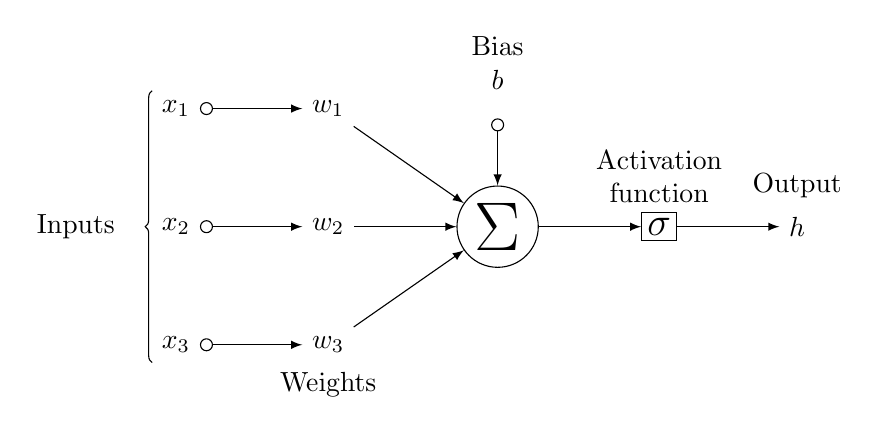
\begin{tikzpicture}[
init/.style={
  draw,
  circle,
  inner sep=2pt,
  font=\Huge,
  join = by -latex
},
squa/.style={
  draw,
  inner sep=2pt,
  font=\Large,
  join = by -latex
},
start chain=2,node distance=13mm
]
\node[on chain=2] 
  (x2) {$x_2$};
\node[on chain=2,join=by o-latex] 
  {$w_2$};
\node[on chain=2,init] (sigma) 
  {$\displaystyle\Sigma$};
\node[on chain=2,squa,label=above:{\parbox{2cm}{\centering Activation \\ function}}]   
  {$\sigma$};
\node[on chain=2,label=above:Output,join=by -latex] 
  {$h$};
\begin{scope}[start chain=1]
\node[on chain=1] at (0,1.5cm) 
  (x1) {$x_1$};
\node[on chain=1,join=by o-latex] 
  (w1) {$w_1$};
\end{scope}
\begin{scope}[start chain=3]
\node[on chain=3] at (0,-1.5cm) 
  (x3) {$x_3$};
\node[on chain=3,label=below:Weights,join=by o-latex] 
  (w3) {$w_3$};
\end{scope}
\node[label=above:\parbox{2cm}{\centering Bias \\ $b$}] at (sigma|-w1) (b) {};

\draw[-latex] (w1) -- (sigma);
\draw[-latex] (w3) -- (sigma);
\draw[o-latex] (b) -- (sigma);

\draw[decorate,decoration={brace,mirror}] (x1.north west) -- node[left=10pt] {Inputs} (x3.south west);
\end{tikzpicture}

\caption{A visualization of a perceptron.}
\label{fig:perceptron}
\end{figure}
which, interestingly, can also be rewritten in terms of tensor operations and that allows us to express the perceptron classification rule as 
\begin{equation}
	f(\vec{x}) = \text{sign}(\vec{w}^\intercal \vec{x} + b).
	\label{eq:tensor_perceptron}
\end{equation}
Eq. \ref{eq:tensor_perceptron} makes it possible to conveniently visualize the mathematical operations of the perceptron through a \textcolor{RoyalBlue}{computational graph}, a directed graph where each node represents a certain mathematical operation. The computational graph of Eq. \ref{eq:tensor_perceptron} is represented in Fig. \ref{fig:computational_graph_0} and can be considered as the main building block of modern artificial neural networks.
\begin{figure}[ht!]
	\centering
	\tikzset{
    ->, 
    level distance = 22em,
    minimum size=2em,
    %edge from parent/.style={draw,thick},
    level 1/.style={sibling distance=6em},
    level 2/.style={sibling distance=3em},
    thick/.style = {line width=1.5pt},
    extra thick/.style = {line width=3.5pt},
    red node/.style={shape=circle,draw=red,fill=red!40,thick,inner sep=1.2},
    blue node/.style={shape=circle,draw=blue,fill=blue!40,thick,inner sep=1.2}
}

\tikzstyle{round}=[thick,draw=black,circle]

 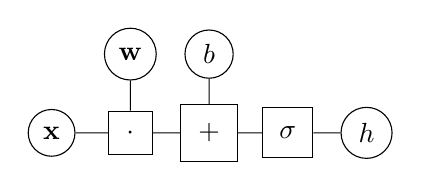
\begin{tikzpicture}[square/.style={regular polygon,regular polygon sides=4}]
	 \node at (0,0) [circle,draw] (input) {$\vec{x}$};
         \node at (1,0) [square,draw] (dot1) {$\cdot$};
	 \node at (1,1) [circle,draw] (W1) {$\vec{w}$};
	 \node at (2,1) [circle,draw] (bias) {$b$};
                  
	 \node at (2,0) [square,draw] (plus) {$+$};	 
	 \node at (3,0) [square,draw] (sigmoid1) {$\sigma$};
	 \node at (4,0) [circle,draw] (h1) {$h$};
         
	 \draw (W1) -> (dot1);
	 \draw (bias) -> (plus);
	 \draw (input) -> (dot1); 
         \draw (dot1)-> (plus); 
         \draw (plus)-> (sigmoid1); 
	 \draw(sigmoid1) -> (h1);
	 
\end{tikzpicture}

	\caption{The computational graph representing the mathematical operations performed by the perceptron represented in Fig. \ref{fig:perceptron} and defined by Eq. \ref{eq:tensor_perceptron}.}
\label{fig:computational_graph_0}
\end{figure}

Eq. \ref{eq:tensor_perceptron} summarizes the computations that are performed by one single input where $\vec{x}\in\mathds{R}^{p}$, $\vec{w}\in\mathds{R}^{p}$ and $b\in\mathds{R}$. However, the computation capabilities of such a single unit are very limited and can rarely be adopted to solve complex tasks. To overcome this, one can stack several units in parallel such that they create a layer with $q$ outputs defined as:
\begin{equation}
	\vec{h} = \sigma(\vec{W}^\intercal\vec{x}+\vec{b}),
\end{equation}
where $\vec{h}\in\mathds{R}^{q},\vec{x}\in\mathds{R}^{p},\vec{W}\in\mathds{R}^{p\times q},b\in\mathds{R}^{q}$. To increase the flexibility and capabilities of the model even further, one can then compose a sequence of $L$ layers
\begin{equation}
	\begin{split}
		\vec{h}_0 & = \vec{x} \\ 
		\vec{h}_1 & = \sigma(\vec{W}^{\intercal}_{1}\vec{h}_0 + \vec{b}_1) \\ 
	... \\
		\vec{h}_L & = \sigma(\vec{W}^{\intercal}_{L}\vec{h}_{L-1}+\vec{b}_{L})
	\end{split}
\end{equation}
and define a \textcolor{RoyalBlue}{multilayer perceptron} (MLP), also known as feedforward neural network. From now on we will refer to an MLP as $f(\vec{x};\theta)$ where $\theta=\{\vec{W}_k,\vec{b}_k,...|k=1,...,L\}$. 

Now that we defined the mathematical computations that are performed by a feedforward neural network we move on to explaining how one can train these kind of models to perform empirical risk minimization.

\subsection{Stochastic Gradient Descent}
\label{sec:sgd}

Training a neural network consists in finding parameters $\theta$ such that a loss function $\mathscr{L}(\theta)$, also denoted as the \textcolor{RoyalBlue}{objective function}, is minimized. Such loss functions are typically expressed as a sum of the losses $\ell_n$ incurred by each sample $n$ in a training set of size $N$, and can be expressed in the following form:
\begin{equation}
	\mathscr{L}(\theta) = \sum_{n=1}^{N}\ell_n(\theta).
	\label{eq:sum_of_losses}
\end{equation}
When neural networks are used, $\mathscr{L}$ has to be differentiable as this allows to minimize it through first order optimization algorithms. Among such methods, the arguably most straightforward one is gradient descent, which updates the parameters $\theta$ proportionally to the negative gradient of $\mathscr{L}$. This is done by applying the following update rule:
\begin{equation}
	\begin{split}
	\theta_{t+1} & = \theta_t - \gamma_t(\nabla\ell(\theta_t))^{\intercal} \\ 
	& = \theta_t - \gamma_t \sum_{n=1}^{N}(\nabla \ell_n(\theta_t))^{\intercal},
	\end{split}
	\label{eq:gradient_descent}
\end{equation}
where $t$ is a time counter variable, and $\gamma\geq0$ is the learning rate, sometimes also denoted as the step-size parameter. We can easily observe that computing Eq. \ref{eq:gradient_descent} can become computationally very expensive as it requires to evaluate gradients from all individual functions $\ell_n$. This property is in fact what defines gradient descent as a batch optimization method, which makes it unfortunately unsuitable for dealing with large datasets. A possible solution to this computational burden consists in reducing the amount of computation required by the sum in Eq.\ref{eq:gradient_descent} by simply considering a small, random batch of samples of the training set. In the extreme case, one can even just estimate the gradient on one single, randomly chosen, training sample, which is a method called Stochastic Gradient Descent (SGD). While it is true that this approach gives an unbiased estimate of the true gradient, its estimate can also be very noisy, which is the reason behind why it is preferable to evaluate the gradient for a mini-batch of samples instead than on one single, unique sample. A large body of work has investigated the effect that the batch-size has on neural network training \cite{keskar2016large,radiuk2017impact,kandel2020effect}; however, so far no exact rule for determining an optimal batch-size exists. Yet, provided that enough computational resources are available, large mini-batches are usually preferred as they will result in more accurate estimates of the gradient, and therefore reduce the variance in the parameter update $\theta_{t+1}$. 

When the optimization surface is made of valley floors, gradient descent has the limitation of being very slow. To deal with such issue, several works have designed optimization strategies which make gradient based optimization faster and more efficient. The most straightforward improvement to the gradient descent algorithm is the one proposed by \citet{rumelhart1986learning} who suggested to use of an additional term in the update rule presented in Eq.\ref{eq:gradient_descent}, named \textcolor{RoyalBlue}{momentum}. This term, simply keeps track of what happened when the parameters were updated at $t-1$ and determines the next parameters' update as a linear combination between the current and previous gradients. This results in the following update rule:
\begin{equation}
	\theta_{t+1} = \theta_t - \gamma_t ((\nabla \ell(\theta_t)))^{\intercal} + \alpha\Delta\theta_t
	\label{eq: momentum}
\end{equation}
where  
\begin{equation}
	\begin{split}
	\theta_{t} & = \theta_t - \theta_{t-1} \\ 
		   & = \alpha\Delta\theta_{t-1}-\gamma_{t-1}(\nabla \ell(\theta_{t-1}))^{\intercal},
	\end{split}
\label{eq:gradient_descent}
\end{equation}
and $\alpha\in[0,1]$, which accelerates the optimization process and allows the algorithm average out noisy estimates of the gradient.

Next to adding a momentum term to improve the performance of gradient descent, another common method that can accelerate its convergence revolves around dynamically adapting the learning rate parameter $\gamma$. Popular neural network optimizers such as \texttt{RMSProp} \cite{tieleman2012lecture}, \texttt{AdaGrad} \cite{duchi2011adaptive}, and the very well-known \texttt{Adam} optimizer \cite{kingma2014adam}, all adapt this method. While discussing these algorithms into detail is out of the scope of this thesis, we refer the reader to the work of \citet{ruder2016overview}, which provides a nice overview of the most common gradient descent optimization algorithms, and to the work of \citet{schmidt2020descending} who empirically evaluate their performance across different networks and machine learning problems. 

Before ending this section it is worth noting that next to SGD-like methods, there also exist several alternative algorithms that can be used for optimization problems. Among such methods, we mention second order optimization techniques such as Newton, Quasi-Newton and the Conjugate gradient methods discussed in \cite{tan2019review}. While these algorithms are able to minimize the empirical risk faster and even better than SGD, they do not result in equally good generalization performance. Recall from Sec. \ref{sec:learning_from_data}, that in SL minimizing the expected risk is just as important as minimizing the empirical risk, which is a property that the aforementioned second order optimization algorithms do not have. This key result, first presented by \citet{bottou201113}, is what motivates the use of SGD-like optimizers in deep learning.       

\subsection{Backpropagation}
\label{sec:backprop}

From Eq. \ref{eq:gradient_descent} we can note that a crucial role in the optimization process is played by the gradient $\nabla\ell(\theta)$. As we have seen in Sec. \ref{sec:general_architecture} neural networks can be considered as a composition of nested functions $k$ for $k=0,...,K-1$, where each function comes with its own parameters $\theta_k$. Therefore the gradient comes in the form of a vector which contains all the partial derivatives of the loss $\ell$ with respect to the weights $\theta$ that parametrize the neural network:
\begin{equation}
	\nabla\ell(\theta) = \Big[\frac{\partial\ell}{\partial\theta_0}(\theta),...,\frac{\partial\ell}{\partial\theta_{K-1}}(\theta)\Big].
\end{equation}
As the number of functions increases, so does the complexity of the gradient, therefore an efficient way of calculating it is necessary. The backpropagation algorithm \cite{linnainmaa1970representation,bryson1975applied,rumelhart1986learning} is a special case of a more general technique, called \textcolor{RoyalBlue}{automatic differentiation} (see \cite{baydin2018automatic} for a general review about the topic), that allows to evaluate the gradient of complicated functions numerically and automatically. This is done by exploiting the chain rule, which can be applied recursively on the computation graph that keeps track of all the arithmetic operations that are performed by the network. 

To this end let us define a simplified version of a two hidden layer perceptron $f$ that is parametrized with weight matrices $\vec{W}_1$ and $\vec{W}_2$. When given input data $\vec{x}$ the network produces a prediction $\hat{y}$ which results from traversing the computational graph represented in Fig. \ref{fig:computational_graph_1}.  
\begin{figure}[ht!]
	\centering
	\tikzset{
    ->, 
    level distance = 22em,
    minimum size=2em,
    %edge from parent/.style={draw,thick},
    level 1/.style={sibling distance=6em},
    level 2/.style={sibling distance=3em},
    thick/.style = {line width=1.5pt},
    extra thick/.style = {line width=3.5pt},
    red node/.style={shape=circle,draw=red,fill=red!40,thick,inner sep=1.2},
    blue node/.style={shape=circle,draw=blue,fill=blue!40,thick,inner sep=1.2}
}

\tikzstyle{round}=[thick,draw=black,circle]

 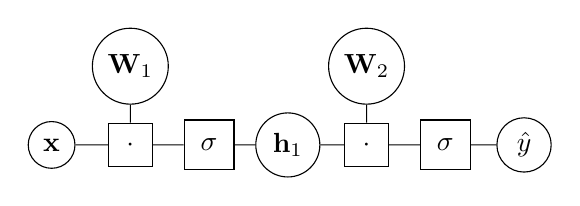
\begin{tikzpicture}[square/.style={regular polygon,regular polygon sides=4}]
	 \node at (0,0) [circle,draw] (input) {$\vec{x}$};
         \node at (1,0) [square,draw] (dot1) {$\cdot$};
	 \node at (1,1) [circle,draw] (W1) {$\vec{W}_1$};
	 \node at (2,0) [square,draw] (sigmoid1) {$\sigma$};
	 \node at (3,0) [circle,draw] (h1) {$\vec{h}_1$};
         \node at (4,0) [square,draw] (dot2) {$\cdot$};
	 \node at (4,1) [circle,draw] (W2) {$\vec{W}_2$};
	 \node at (5,0) [square,draw] (sigmoid2) {$\sigma$};
	 \node at (6,0) [circle,draw] (output) {$\hat{y}$};

	 \draw (W1) -> (dot1);
	 \draw (W2) -> (dot2);
	 \draw (input) -> (dot1); 
	 \draw (dot1)-> (sigmoid1); 
	 \draw(sigmoid1) -> (h1);
	 \draw(h1) -> (dot2); 
	 \draw(dot2) -> (sigmoid2);
	 \draw(sigmoid2)-> (output);  

\end{tikzpicture}

	\caption{The computational graph representing a simplified version of a multi-layer perceptron with one hidden layer. Note that no bias term is added after multiplying $\vec{x}$ and $\vec{h1}$ by $\vec{W_1}$ and $\vec{W}_2$ respectively.}
\label{fig:computational_graph_1}
\end{figure}
During the traversal, also known as the \textcolor{RoyalBlue}{forward pass}, the result of each mathematical operation is stored within its own output variable $u$ (see Fig. \ref{fig:computational_graph_2}) 
\begin{figure}[ht!]
	\centering
	\tikzset{
    ->, 
    level distance = 22em,
    minimum size=2em,
    %edge from parent/.style={draw,thick},
    level 1/.style={sibling distance=6em},
    level 2/.style={sibling distance=3em},
    thick/.style = {line width=1.5pt},
    extra thick/.style = {line width=3.5pt},
    red node/.style={shape=circle,draw=red,fill=red!40,thick,inner sep=1.2},
    blue node/.style={shape=circle,draw=blue,fill=blue!40,thick,inner sep=1.2}
}

\tikzstyle{round}=[thick,draw=black,circle]

 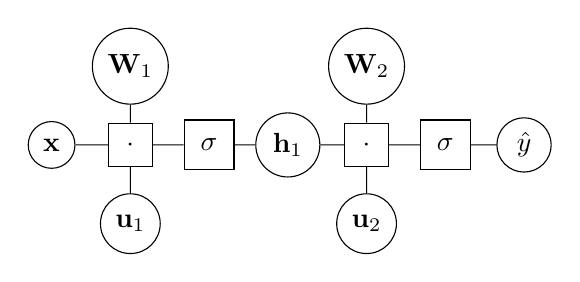
\begin{tikzpicture}[square/.style={regular polygon,regular polygon sides=4}]
	 \node at (0,0) [circle,draw] (input) {$\vec{x}$};
         \node at (1,0) [square,draw] (dot1) {$\cdot$};
	 \node at (1,1) [circle,draw] (W1) {$\vec{W}_1$};
	 \node at (1,-1) [circle,draw] (o1) {$\vec{u}_1$};
	 \node at (2,0) [square,draw] (sigmoid1) {$\sigma$};
	 \node at (3,0) [circle,draw] (h1) {$\vec{h}_1$};
         \node at (4,0) [square,draw] (dot2) {$\cdot$};
	 \node at (4,1) [circle,draw] (W2) {$\vec{W}_2$};
 	 \node at (4,-1) [circle,draw] (o2) {$\vec{u}_2$};
	 \node at (5,0) [square,draw] (sigmoid2) {$\sigma$};
	 \node at (6,0) [circle,draw] (output) {$\hat{y}$};

	 \draw (W1) -> (dot1);
	 \draw (W2) -> (dot2);
	 \draw (input) -> (dot1); 
	 \draw (dot1)-> (sigmoid1); 
	 \draw (dot1)-> (o1); 
	 \draw(sigmoid1) -> (h1);
	 \draw(h1) -> (dot2); 
	 \draw(dot2) -> (sigmoid2);
         \draw (dot2)-> (o2);
	 \draw(sigmoid2)-> (output);  

\end{tikzpicture}

	\caption{The computational graph that results after having performed one forward pass through the network. We can see that the result of each mathematical operation is stored within a new node $\vec{u}$ that will be necessary for computing the partial derivatives required to perform stochastic gradient descent.}
\label{fig:computational_graph_2}
\end{figure}
Having such an annotated graph it is now possible to compute all partial derivatives efficiently by traversing the graph backwards (\textcolor{RoyalBlue}{backward pass} \cite{linnainmaa1970representation}), and by applying the chain rule which in its general form states that:
\begin{equation}
	\frac{\text{d} \ell}{\text{d} \theta_i} = \sum_{k\in\text{parents}(\ell)} \frac{\partial \ell}{\partial u_k} \frac{\partial u_k}{\partial \theta_i}.
\end{equation}
Therefore taking as example $\vec{W}_1$, the derivative of the network's output $\hat{y}$ with respect to this weight matrix is given by:
\label{eq:general_chain_rule}
\begin{equation}
	\begin{split}
		\frac{\text{d} \hat{y}}{\text{d} \vec{W}_1} & = \frac{\partial \hat{y}}{\partial u_2} \frac{\partial u_2}{\partial h_1} \frac{\partial h_1}{\partial u_1} \frac{\partial u_1}{\partial\vec{W}_1} \\
	& = \frac{\partial\sigma(u_2)}{\partial u_2} \frac{\partial\vec{W}_2^{\intercal}h_1}{\partial h_1} \frac{\partial \sigma(u_1)}{\partial u_1} \frac{\partial \vec{W}_1^{\intercal}\vec{x}}{\partial{\vec{W}_1}}.
	\end{split}
	\label{eq:applied_chain_rule}
\end{equation}

\subsection{Loss Functions}
\label{sec:loss_functions}
Defining an appropriate loss function is a task that has important practical implications when it comes to the design of the neural architecture. Just like for any other type of machine learning model, the choice of which loss function to minimize depends from the SL task we would like to solve. Fortunately, since neural networks are parametric models, their loss functions are not too different from the ones that are typically used by e.g.,  linear models such as . The most important concept underlying the loss functions used by neural networks is that of \textcolor{RoyalBlue}{maximum likelihood estimation}. As many other parametric models, neural networks implicitly define a distribution $p(Y|\vec{x};\theta)$. This is convenient as it makes it possible to exploit the cross-entropy between the training data and the model's predictions. Therefore, no matter whether we are dealing with a classification problem or a regression one, the loss function that will be adopted by a neural network will always come in the following general form:
\begin{equation}
	\mathscr{L}(\theta) = - \mathds{E}_{(\vec{x},y)\sim P(X,Y)} \log p_\text{model} (Y|\vec{x}).
	\label{eq:maximum_likelihood}
\end{equation}

Typical loss functions that derive from Eq. \ref{eq:maximum_likelihood} (see Chapter 5 of \cite{goodfellow2016deep} for the exact derivations) are the mean squared error (MSE) loss
\begin{equation}
	\mathscr{L}(\theta) = \frac{1}{2}\mathds{E}_{(\vec{x},y\sim P(X,Y))} ||y - f(\vec{x};\theta) ||^{2}
	\label{eq:mean_squared_error}
\end{equation}
which is used for tackling regression problems, and the categorical cross-entropy loss
\begin{equation}
	\mathscr{L}(\theta) = - \mathds{E}_{(\vec{x},y\sim P(X,Y))} \sum_{i=1}^{C} y^{i} \log f(\vec{x};\theta)
	\label{eq:cross_entropy}
\end{equation}
which is used for multi-class classification problems, where $C$ is the number of classes we would like to classify. 

Based on whether Eq. \ref{eq:mean_squared_error} or Eq. \ref{eq:cross_entropy} is minimized, the final layer of a neural network comes in different forms. As the goal of a regression problem is to predict a single numerical value, it follows that the final layer simply consists of one individual unit that is necessary for estimating $\mathcal{Y}\in\mathds{R}$. One single output unit is also used for binary classification problems, where it is combined with the sigmoid activation function
\begin{equation}
	\sigma(x) = \frac{1}{1+\exp(-1)}
	\label{eq:sigmoid}
\end{equation}
which allows to model a Bernoulli distribution over a binary variable. For classification problems, where $C>2$, and the goal is to represent the distribution over a discrete variable that can have $C$ possible values, the sigmoid function can be generalized to a softmax function by producing a vector for $i=1,...,C$ such that:
\begin{equation}
	\text{Softmax}(\vec{z})_i = \frac{\exp(z_i)}{\sum_{j=1}^{C} \exp(z_j)}.
	\label{eq:softmax}
\end{equation}
We can observe that Eq. \ref{eq:softmax} makes the log probabilities, typically estimated by the second-last layer of a network, positive and sum up to one, therefore successfully modeling a multinoulli distribution. While the aforementioned output layers are arguably the most popular it is worth noting that several other types of output layers exist. Since throughout this dissertation none of these additional layers will be used in practice we will not describe them here and refer the reader to Chapter 6 of \cite{goodfellow2016deep} for more information about this topic.

\subsection{Vanishing Gradients and Activation Functions}
\label{sec:activation_functions}

A typical problem of neural networks that come with many hidden layers is given by vanishing gradients. Recall from Sec. \ref{sec:backprop} that in order to perform SGD we first need to collect all the partial derivatives of the network's output with respect to its parameters. As we do this by applying the chain rule this can have the drawback of making the gradient decrease exponentially with respect to the depth of the network. As a result deeper layers can become particularly hard to train, since no information necessary for updating the respective weights will be contained within the gradient. The most common cause of this problem is given by the activation function that is used for introducing non-linearity across the network. For example, let us consider the sigmoid function presented in Eq. \ref{eq:sigmoid} and its derivative which comes in the following form:
\begin{equation}
	\frac{\text{d}\sigma}{\text{d}x}(x) = \sigma(x)(1-\sigma(x)).
	\label{eq:derivative_sigmoid}
\end{equation}
As we can see from the first image of Fig. \ref{fig:activation_functions}, the maximum value of Eq. \ref{eq:derivative_sigmoid} is 0.25. If we then use this value when adopting the chain rule as done in Eq. \ref{eq:applied_chain_rule}, and assume the network comes with a large number of hidden layers, it is easy to see that the gradient $\frac{\text{d}\hat{y}}{\text{d}\vec{W}_1}$ will shrink to zero as the number of layers increases. The sigmoid function is not the only activation function which suffers from this phenomenon, which is also not restricted to feedforward neural networks. In fact as first presented by \citet{} another non-linear activation function suffering from the vanishing gradient problem is the hyperbolic tangent 
\begin{equation}
	\text{tanh}(x) = \frac{1-\exp(-2x)}{1+\exp(-2x)}.
\end{equation}
As can be seen in the second plot of Fig. \ref{fig:activation_functions} the tanh is very similar in shape to the sigmoid. This activation function is largely used within Recurrent Neural Networks (RNNs), a particular type of neural network that can be unfolded into very deep MLPs. For many years its vanishing gradient issues have questioned whether RNNs could be trained and used in practice, a problem which has been successfully solved with the introduction of the Long Short Term Memory (LSTM) cells \cite{hochreiter1997long}. 

\begin{figure}[ht!]
	\centering
	\begin{tikzpicture}[scale = 1]
\begin{axis}[
grid style={dashed,gray},
grid = both, 
  legend pos=north west]

\addlegendentry{ReLU}
\addplot [ultra thick, blue] table [y=Relu, x=P]{./Images/Chapter01/activation_functions.dat};
\addlegendentry{Elu}
\addplot [ultra thick, red] table [y=Elu, x=P]{./Images/Chapter01/activation_functions.dat};
\addlegendentry{Tanh}
\addplot [ultra thick, black] table [y=Tanh, x=P]{./Images/Chapter01/activation_functions.dat};
\addlegendentry{Sigmoid}
\addplot[ultra thick, green] table [y=Sigmoid, x=P]{./Images/Chapter01/activation_functions.dat};
\end{axis}
\end{tikzpicture}



	\caption{In the left plot a visualization of the vanishing gradient problem that can come from using a sigmoid non-linear activation function throughout a network. In the right plot a representation of typical non-linear activation functions within the $[-3,3]$ range that are currently used by popular neural architectures.}
\label{fig:activation_functions}
\end{figure}

Another solution to the vanishing gradient problem is to use the Rectified Linear Unit (ReLU) activation function (represented in green in Fig. \ref{fig:activation_functions}), which is arguably the most popular choice when it comes to the design of deep neural networks. This activation function is simply defined as
\begin{equation}
	\text{ReLU}(x) = \max(0,x).
\end{equation}
Its derivative has the appealing property of staying constant to 1 whenever a unit is activated as defined by: 
\begin{equation}
	\frac{\text{d}}{\text{d}x} \text{ReLU}(x) = \begin{cases} 0 & \text{if } x \leq 0 \\ 1 & \text{otherwise} \end{cases}
\end{equation}

A potential drawback of ReLU is that whenever its input is negative gradient based methods could not be used for learning, as the unit will have a value of 0. To overcome this several activation functions that generalize the ReLU to negative inputs have been proposed within the literature \cite{clevert2015fast, maas2013rectifier, he2015delving}, among which we mention the Elu \cite{clevert2015fast} that is visually represented in red in the last plot of Fig. \ref{fig:activation_functions}. 


\section{Convolutional Neural Networks}
\label{sec:convolutional_networks}

Convolutional Neural Networks (CNNs) are a family of artificial neural networks that are particularly well suited for problems involving high-dimensional inputs such as images or videos. This kind of data in fact prohibits the use of the multi-layer perceptrons presented in Sec. \ref{sec:general_architecture}, as it requires to represent images as unstructured vectors, which is a process that for obvious computational reasons is not feasible. Furthermore MLPs present some additional limitations: first and foremost, due to their fully connected structure, they do not involve any sort of parameter sharing across the network. Second, as the output of each unit in a layer is given as input to all the units in the subsequent layer, the interaction among all such neurons is also extremely dense. CNNs address these limitations by exploiting \textcolor{RoyalBlue}{sparse weight sharing} strategies that result into neural networks that are significantly more memory and computationally efficient. 

\subsection{Mathematical Operations}
\label{sec:operations}

As their name suggests, the key mathematical operation behind CNNs is that of \textcolor{RoyalBlue}{convolution}. A convolution operation is performed over two arguments: an input vector $\vec{x}\in\mathds{R}^{W}$, and a kernel $\vec{u}\in\mathds{R}^{w}$. Its output is a new vector of size $W-w+1$ such that:
\begin{equation}
	(\vec{x}\circledast\vec{u}[i]) = \sum_{m=0}^{w-1}x_{m+i}u_m,
	\label{eq:convolution}
\end{equation}
where $\circledast$ technically denotes the cross-correlation operation, namely a convolution operation that does not flip the kernel. The process described in Eq. \ref{eq:convolution} can easily be generalized to multi-dimensional tensors such as images which can in fact be seen as three-dimensional tensors $\vec{x}\in\mathds{R}^{C,W,H}$, of width and height $W$ and $H$ respectively, defined over the RGB color domain ($C=3$). Similarly one can also define a three-dimensional kernel $\vec{u}\in\mathds{R}^{C,w,h}$ whose purpose is to slide over the input tensor $\vec{x}$ and which yields a two-dimensional output tensor $\vec{o}$ of size $(H-h+1)\times(W-1+1)$ that is computed as follows:
\begin{equation}
	\begin{split}
		\vec{o}_{i,j} & = \vec{b}_{i,j} + \sum_{c=0}^{C-1}(\vec{x}_c\circledast\vec{u}_c)[j,i] \\ 
			      & = \vec{b}_{i,j} + \sum_{c=0}^{C-1} \sum_{n=0}^{h-1}\sum_{m=0}^{w-1} \vec{x}_{c,n+j,m+i}\vec{u}_{c,n,m},
	\end{splot}
\end{equation}
where $\vec{b}$ and $\vec{u}$ are learnable parameters. Within the deep learning literature, $\vec{o}$ is also referred to as a \textcolor{RoyalBlue}{feature map} \cite{goodfellow2016deep}.

Note that by adopting a convolution approach, one input unit in the network only affects as many output units as defined by the size of the kernel, which improves the computational efficiency of the network greatly. Furthermore, each member of the kernel is used across the entire image, which means that the parameters that define a convolution operation are shared alongside the different locations that are visited by $\vec{u}$. The way the kernel interacts with its respective tensor is usually defined by two additional components that both play an important role in the design of convolutional networks. The first of these components is \textcolor{RoyalBlue}{padding} which is a technique that adds some extra values around the perimeter of the input tensor $\vec{x}$, with the aim of preserving the information that is depicted around its corners. Second, there is the concept of \textcolor{RoyalBlue}{strides} which defines by how many elements at a time we wish to slide $\vec{u}$ over $\vec{x}$. As the goal of CNNs is that of downsampling the input tensor in a computationally efficient manner, it is usually good practice to have strides larger than one, albeit this comes at the cost of extracting features less thoroughly. 

Convolutional networks typically perform several convolutions in parallel, as multiple kernels are used. The output of each convolution is then passed through a non linear activation function such as the ones that we represented in Fig. \ref{fig:activation_functions}. To downsample the resulting feature maps even further, a \textcolor{RoyalBlue}{pooling} function is usually adopted. Its idea is to summarize the output of the convolving process at a certain location of the feature map through a summary statistic. This reduces its size while at the same time preserves the presence of the detected features. There are two common pooling operations one can choose from: max-pooling \cite{zhou1988computation}, which given a three dimensional tensor $\vec{x}\in\mathds{R}^{C\times(rh)\times(sw)}$ produces a tensor $\vec{o}\in\mathds{R}^{C\times r\times s}$ by simply keeping the maximum value of a feature map within a certain rectangular neighborhood such that 
\begin{equation}
	\vec{o}_{c,j,i} = \underset{n<h,m<w}{\max} \vec{x}_{c,rj+n,si+m},
\end{equation}
and average pooling, which instead computes the mean of a feature map such that 
\begin{equation}
	\vec{o}_{c,j,i} = \frac{1}{hw} \sum_{n=0}^{h-1}\sum_{m=0}^{w-1} \vec{x}_{c,rj+n,si+m}.
\end{equation}
Besides reducing the size of a feature map, pooling operations have also the important benefit of making the representations learned by the network invariant to small translations. In fact, one could translate the input by a small amount and still obtain the same output after pooling. Note however, that albeit desirable in most cases, there are situations where adopting pooling strategies should be avoided \cite{sabatelli2018learning, bidoiadeep}.  


\subsection{Popular Architectures}
\label{sec:architectures}

With all these concepts in place we can now define the general structure of a convolutional neural network. These models follow a general pattern, originally described in \cite{lecun1998gradient}, which is in principle very simple: an input tensor is processed by the aforementioned convolution operation, which is done for many times in parallel, as different kernels are typically used. The resulting feature map is then given as input to one of the non-linear activation functions described in Sec. \ref{sec:activation_functions}, among which the ReLU is by far the most popular choice, as it allows to control the vanishing gradient problem. The resulting feature map is then reduced by performing one of the aforementioned pooling operations. This process of convolving + ReLU + pooling is repeated several times, until the feature map is small enough to be reduced to a feature vector. This feature vector is finally processed by either a multilayer perceptron, or directly by the last output layer of the network, which as described in Sec. \ref{sec:loss_functions}, changes with respect to the SL we would like to solve. While this general principle has arguably barely changed over the last two decades, it is worth noting that several design choices have been proposed over the years with the aim of creating better performing, and increasingly more efficient models. We will review some of the most important ones hereafter.  

\paragraph{Image Classification Networks}

The first successful application of a convolutional neural network dates back to 1998, when \citet{lecun1998gradient} introduced \texttt{LeNet-5}, a 5-layer deep network which achieved state-of-the-art results on the MNIST handwriting recognition benchmark. Despite its success however, convolutional neural networks did not gain much popularity for over ten years. In fact, the largely limiting computational resources of the time, prevented them to successfully tackle image classification challenges more complicated than the aforementioned MNIST dataset. Only in 2012, with the introduction of \texttt{AlexNet} \cite{krizhevsky2012imagenet}, convolutional networks started to grab the spotlight within the computer vision community.  The work of \citet{krizhevsky2012imagenet}, resulted in an 8-layer convolutional network, which combined with a 3-layer multilayer perceptron, achieved state-of-the-art results on the ImageNet Large Scale Visual Recognition Challenge (ILSVRC), a popular computer vision dataset which we will review in more detail in Chapter \ref{ch:transfer_learning}. Among the main contributions of their work we mention the first results reporting the possibility of applying convolutional networks to largely more complicated computer vision tasks, and the possibility of training these models in a distributed fashion by exploiting, at least partially, the potential benefits of parallel computing. The advent of better specialized hardware, among which we mention the development of increasingly powerful Graphical Power Units (GPUs), together with the successful results obtained by \texttt{AlexNet}, convinced the machine learning community to explore the potential benefits of convolutional networks further. The most promising line of work was certainly pioneered by Oxford's University Visual Geometry Group (VGG) which investigated whether deeper networks could yield better performance. Their \texttt{VGG16} and \texttt{VGG19} models \cite{simonyan2014very}, of depth 16 and 19 respectively, showed that this was indeed the case, a design choice which combined with the use of smaller kernels allowed these models to outperform \texttt{AlexNet}. Similar results were almost concurrently achieved by \citet{szegedy2015going} who introduced \texttt{GoogLeNet}, a convolutional network that uses the notion of Inception-Blocks, a specific form of convolutional layer which simultaneously uses kernels of different sizes. Among these kernels we mention the use of $1\times1$ convolutions which have the appealing benefit of acting as a powerful dimensionality reduction technique. While all these networks are certainly deeper than \texttt{LeNet-5}, their number of hidden layers is on average around a dozen. Despite adopting ReLU activation functions all the aforementioned networks do still happen to suffer from the vanishing gradient problem. \citet{he2016deep} successfully addressed this limitation by introducing the concept of residual blocks and skipped connections. They propose to use the output of one convolutional layer $l$, not only as input to the immediate subsequent layer $l+1$, but also to some of the subsequent layers e.g., $l+2$ and $l+3$. This simple, yet very effective trick, allowed \citet{he2016deep} to build \texttt{ResNets}, convolutional networks consisting of up to 152 layers which significantly outperformed \texttt{GoogLeNet}. \citet{huang2017densely} built on top of their ideas and introduced \texttt{DenseNets}, which take the concept of skipped connections to another level, by designing models where each layer in the network takes as input the feature maps computed by all the predecessor layers. While the models presented so far are arguably the most popular ones, as they outperformed each other over the years when the ILSVRC was still an on-going yearly competition, is should be noted that many more, equivalently successful networks have been proposed over the years. Among such networks we mention \texttt{Inception-ResNets}, which combine inception and residual blocks \cite{szegedy2017inception} and \texttt{MobileNets} \cite{sandler2018mobilenetv2, howard2019searching} and \texttt{EfficientNet} \cite{tan2019efficientnet,}, which are models that are specifically built for minimizing inference time on devices with limited hardware capabilities. 

\paragraph{Beyond Image Classification}



\section{Conclusion}
\label{sec:conclusion01}
In this chapter we have introduced supervised learning, and seen what it means to build statistical models that are able to capture the interaction between input-output observations. We have specifically focused on algorithms that come in the form of artificial neural networks as this is the type of learning algorithms that, to this date, are by far the most successful ones. Interestingly, their learning capabilities are not limited to supervised learning problems only, which means that artificial neural networks can also be used for machine learning problems that do not strictly require building empirical risk minimizers. Among such problems we mention the ones that are modeled by reinforcement learning, a branch of machine learning which throughout this dissertation will receive as much attention as supervised learning and that will be presented in the coming chapter.
 % Supervised Learning + Deep Learning
\chapter{Reinforcement Learning and Deep Neural Networks}
\label{ch:reinforcement_learning}


\begin{remark}{Outline}
This chapter introduces the research field of Reinforcement Learning (RL) and presents how its algorithms can successfully be combined with neural networks. The successful marriage between RL and deep neural networks comes with the name of Deep Reinforcement Learning (DRL) and builds on top of research that dates back to a time when training neural networks was not the common practice it is nowadays. We start by providing a general introduction to the field of RL in Sec. \ref{sec:rl_introduction} where we describe the main objectives of this machine learning paradigm and see how it differs from the supervised learning setting that we have described in the previous chapter. We then present the mathematical framework that underpins the development of RL algorithms in Sec. \ref{sec:mdps}, \ref{sec:goals_and_returns} and \ref{sec:value_functions}. In Sec. \ref{sec:learning_value_functions} and Sec. \ref{sec:function_approximators} we describe how one can create RL algorithms and why it is desirable to integrate the resulting algorithms with neural networks. In Sec. \ref{sec:deep_reinforcement_learning} we describe the field of DRL and introduce some of the most popular techniques that have been proposed over the years. This chapter ends with Sec. \ref{sec:challenges} where we discuss one of the main challenges that currently characterizes DRL and that has served as inspiration for the research that will be presented in Chapters \ref{ch:dqv_family_of_algorithms} and \ref{ch:dqn_transfer} of this dissertation.

\end{remark}

\section{Introduction}
\label{sec:rl_introduction}
In Chapter \ref{ch:supervised_learning}, we have described Supervised Learning (SL), a machine learning framework that aims at constructing models which can answer statistical questions about data coming in the form of input-output pairs. When these models are built successfully, it is possible to use them to make predictions about the behavior of new unseen data. Training SL models is a process which from some perspective is very static. Datasets are divided into training, validation, and testing sets, and besides providing a model with a large set of samples drawn from these datasets, there is no real interaction between the learning algorithm and the data that drives the learning process. In Reinforcement Learning (RL), this changes drastically. The goal is not to learn a mapping between a set of fixed input samples and their respective targets, but to train an algorithm that learns how to interact with an environment. RL is, therefore, a much more dynamic learning paradigm, where the concept of time is omnipresent and is critical for the development of algorithms that not only need to solve a specific problem, but additionally, also have to be able to adapt themselves while training progresses.

In RL, a learning algorithm is usually called the \textcolor{RoyalBlue}{agent}, and it can come in numerous forms: it can range from being a self-driving car that needs to learn how to drive; to a recommendation system whose goal is to propose products to users navigating the web. More generally, we define an RL agent as any system that, given a specific situation, has to choose which action to perform. However, there is one more additional component that makes RL the challenging machine learning setting it is.
It is not enough for an agent to just learn how to interact with the environment, it is even more desirable for it to learn an interaction which can be defined as "intelligent". Going back to the self-driving car example, an "intelligent" agent would not only be a car that can drive autonomously, but a car that is also able to do this while complying with the driving code. Because of this concept of learning how to make (intelligent) decisions while interacting, the problems tackled by RL algorithms are also reffered to as optimal decision making problems, which are also the target of research fields other than machine learning, such as control theory. Interestingly, both worlds try to solve the same set of problems, one by tackling them through algorithms that are denoted as "intelligent", while the other through the development of algorithms that are "optimal." Throughout this dissertation, we will not make a clear distinction between these two worlds and will assume that algorithms yielding intelligent behaviors also result in optimal behaviors. Nevertheless, we encourage the reader that has finished reading this chapter to assess whether acting optimally necessarily coincides with acting intelligently.

\section{Markov Decision Processes}
\label{sec:mdps}

Before starting to develop RL algorithms for sequential decision making problems, we formulate the problem within the mathematical framework of Markov Decision Processes (MDPs) \cite{puterman1990markov,puterman2014markov}. Throughout this dissertation, we will characterize MDPs, and the resulting RL concepts, by using the mathematical notation that was used by \citet{sutton2018reinforcement} in their seminal book about RL, although it is worth noting that within the literature, different formulations can be found for expressing the same kind of concepts \cite{bertsekas1995neuro,busoniu2010reinforcement,bertsekas2000dynamic,bertsekas2019reinforcement}.

We start by introducing the following elements:
\begin{itemize}
	\item A set of possible states $\mathcal{S}$, that can be visited by an agent while it is interacting with the MDP, where $s_t \in \mathcal{S}$ denotes the state being visited at time-step $t$.
	\item A set of possible actions $\mathcal{A}$ that are available to the agent when it is in a certain state, where $a_t \in \mathcal{A}(s_t)$ denotes the action that is performed by the agent in state $s$ at time-step $t$.
\item A transition function $\mathcal{P}:\mathcal{S}\times\mathcal{A}\times\mathcal{S}\rightarrow [0,1]$ that defines the probability for an agent to visit state $s_{t+1}$, based on its current state and the action which will be performed thereafter.
\item A reward function $\Re:\mathcal{S}\times\mathcal{A}\times\mathcal{S}\rightarrow \mathbb{R}$ which returns a reward signal $r_{t}$ when an agent performs action $a_t$ in state $s_t$ and transits to $s_{t+1}$.
\item A discount factor denoted as $\gamma \in [0,1]$ (explained in Section \ref{sec:goals_and_returns}).

\end{itemize}

Based on these concepts a MDP is defined by the following tuple $\langle\mathcal{S}, \mathcal{A}, \mathcal{P}, \Re, \gamma\rangle$ and is also commonly denoted in the RL literature as the \textcolor{RoyalBlue}{environment}. The way the agent interacts with this environment is given by its \textcolor{RoyalBlue}{policy} $\pi$, defined as a probability distribution over $a \in \mathcal{A}(s)$ for each $s \in \mathcal{S}$:
\begin{equation}
	\pi(a|s) = \text{Pr}\; \{a_t = a | s_t = s\}, \; \text{for all}\; s \in \mathcal{S}\; \text{and}\; a\ \in \mathcal{A}. 
\end{equation}
Policies can be deterministic if $\forall s: \pi(a|s) = 1$ for exactly one $a\in \mathcal{A}(s)$ and $\pi(b|s) = 0$ for all $b\in \mathcal{A}(s)\setminus\{a\}$. A policy is also stationary if it does not change over time.

%or stationary, in both cases we can define them as follows:
%\begin{definition}
%	A policy $\pi:\mathcal{S}\rightarrow\mathcal{A}$ is a mapping from states to actions. 
%\end{definition}

The elements of the MDP allow us to properly model the dynamics of an agent interacting with its environment, an interaction which can be summarized as follows: at each time-step $t$ the environment provides the agent with a certain state $s_t$, the agent then performs action $a_t$ which results into the reward signal $r_{t}$. After performing such action the agent will enter into a new state $s_{t+1}$. This continuous interaction with the environment is also known as the Reinforcement Learning loop, and can technically be infinite. However, this is never the case in practice, as an agent will eventually visit a state (denoted as terminal) that only transits to itself, which will therefore stop the agent-environment interaction. We visually represent the Reinforcement Learning loop in Fig. \ref{fig:rl_loop}.

\begin{figure}[htb!]
	\centering
	\tikzset{
  frame/.style={
    rectangle, draw,
    text width=6em, text centered,
    minimum height=4em,drop shadow,fill=white,
    rounded corners,
  },
  line/.style={
    draw, -{Latex},rounded corners=3mm,
  }
}

\begin{tikzpicture}[font=\small\sffamily\bfseries,very thick,node distance = 4cm]
\node [frame] (agent) {Agent};
\node [frame, below=1.2cm of agent] (environment) {Environment};
\draw[line] (agent.0) -- ++ (1.5,0) |- (environment.0) 
node[right,pos=0.25,align=left] {action\\ $a_t$};
\coordinate[left=8mm of environment] (P);
\draw[thin,dashed] (P|-environment.north) -- (P|-environment.south);
\draw[line] (environment.200) -- (P |- environment.200)
node[midway,above]{$s_{t+1}$};
\draw[line,thick] (environment.160) -- (P |- environment.160)
node[midway,above]{$r_{t+1}$};
\draw[line] (P |- environment.200) -- ++ (-1.4,0) |- (agent.160)
node[left, pos=0.25, align=right] {state\\ $s_t$};
\draw[line,thick] (P |- environment.160) -- ++ (-0.8,0) |- (agent.200)
node[right,pos=0.25,align=left] {reward\\ $r_t$};
\end{tikzpicture}


\caption{A visual representation of how an agent interacts with an environment as modeled by a Markov decision process. Figure inspired by page 48 of the \citet{sutton2018reinforcement} textbook.}
  \label{fig:rl_loop}
\end{figure}

Each interaction of the agent with the environment is defined as an \textcolor{RoyalBlue}{episode}, which consists of one or several trajectories $\tau$ that come in the form of the following sequence:
\begin{align}
	\langle(s_t,a_t,r_t,s_{t+1})\rangle,t=0,\ldots,T-1
\end{align}
where $T$ is a random variable representing the length of the episode.

A key property of the environment is that it fulfills the Markov property which is defined as follows:
\begin{definition}
	A discrete stochastic process is Markovian if the conditional distribution of the next state of the process only depends from the current state of the process.
\end{definition}
This implies that the only information that is necessary for predicting to which state an agent will step next are $s_t$ and $a_t$, a concept which can be expressed formally as:
\begin{align}
	p(s_{t+1}|s_t, a_t, s_{t-1}, a_{t-1}, \ldots) = p(s_{t+1} | s_t, a_t).
\end{align}
Interestingly, the same property is also assumed for the reward that the agent will get, meaning that the reward that an agent obtains is only determined by its previous action, and not by the history of all previously taken actions, as defined by:
\begin{align}
	p(r_t| s_t, a_t, \ldots, s_1, a_1) = p(r_t|s_t,a_t).
\end{align}


\section{Goals and Returns}
\label{sec:goals_and_returns}
So far, we have defined all the elements that model an agent's interaction with an environment while introducing some of its fundamental properties. However, we do not yet know what the purpose of this interaction is. In RL, an agent's goal is defined with respect to the reward signal $r_t$ that is returned by the reward function $\Re$ and is very straightforward: maximizing the total amount of reward it receives while interacting with the environment. In the simplest case, we can define this as:
\begin{align}
	G_t = r_t + r_{t+1} + r_{t+2} + \ldots + r_{T}.
\label{eq:goal}
\end{align}
While simple and intuitive, this formulation has one major drawback: it treats each reward signal equally as it does not distinguish rewards that are obtained in the near future, $r_t$, from the ones that will be obtained in the more distant future, $r_{T-1}$. To deal with this issue, we need an additional concept known as \textcolor{RoyalBlue}{discounting}, and that is governed by the discount rate parameter $\gamma$, also known as the discount factor. $\gamma$ allows us to weight the different reward signals based on how close or distant in the future these rewards are received by the agent. By introducing $\gamma$ in Eq. \ref{eq:goal} we can now define the expected discounted return as:
\begin{equation}
	\begin{split}
	G_t & = r_t+\gamma r_{t+1} + \gamma^{2} r_{t+2} + ... \\
	    & = \sum_{k=0}^{\infty}\gamma^{k} r_{t+k}.
	\end{split}
\label{eq:discounted_return}
\end{equation}
The role of $\gamma$ can be interpreted as follows: a reward obtained $k$ time steps in the future is only worth $\gamma^{k-1}$ times what it would be worth if received immediately. It is easy to see how different $\gamma$ values can result in different agent's behaviors. If $\gamma=0$ an agent will only take into account immediate rewards, therefore aiming to maximize $r_{t+1}$ only and resulting into having a "myopic" behavior. If $\gamma$ approaches $1$ the agent will become more "far-sighted", it will take future rewards into account more strongly and will therefore increase its chances of accessing rewards that will result into a higher cumulative return. 
Please note that by defining $\gamma < 1$, we can make the infinite sum presented in Eq. \ref{eq:discounted_return} finite as long as the rewards $r_k$ are bounded.

While the role of $\gamma$ is often taken for granted within the RL literature, it is worth noting that as mentioned by \citet{hessel2019inductive} and \citet{schmidhuber2019reinforcement}, $\gamma$ is an artificial concept that is not present in fields such as traditional control theory or engineering. This is because $\gamma$ corresponds to a concept that does not exist in the real world and that in practice distorts the actual value of $r_t$ in an exponentially shrinking fashion. Even if it is considered standard practice to include a discount factor in the development of RL algorithms, it is worth noting that making $\gamma$ part of the RL framework corresponds to including a form of "inductive bias" within the resulting algorithms. It is common knowledge that low discount factors result in poor performance and that it is therefore beneficial to set $\gamma$ as close to $1$, yet choosing an appropriate $\gamma$ parameter can be more challenging than expected, especially when RL algorithms are combined with function approximators. For example, \citet{wiering2009qv} show that different algorithms prefer different discount factors, while \citet{franccois2015discount} show the benefits of initially starting with a low discount factor which gradually gets increased while training progresses. Finally, \citet{vanseijen2019using} introduce a method that allows the use of low discount factors for approximate RL algorithms while at the same time highlighting that the common perception of the role of $\gamma$ might need revision from the RL community. We discuss an alternative perspective to solving RL problems that does not involve the role of $\gamma$ in Appendix \ref{ch:appendixupsidedown}.             

\section{Value Functions}
\label{sec:value_functions}
We are now ready to introduce the arguably most important concept underlying many RL algorithms: the concept of \textcolor{RoyalBlue}{value}. We can define the value of a state $s$, as well as the value of a specific policy $\pi$ or of a particular action $a$, anyhow, independently from what we are considering, the notion of value is always directly linked to the concept of expected discounted return defined in Eq. \ref{eq:discounted_return}. Given an MDP and a policy $\pi$, we can determine the value of a state $s$ as a function $V^\pi:\mathcal{S}\rightarrow\mathbb{R}$ that measures the expected return that the agent will receive when starting in $s$ and following $\pi$ thereafter. 
\begin{align}
    V^{\pi}(s)=\mathds{E}\bigg[\sum_{k=0}^{\infty}\gamma^{k}r_{t+k}\bigg| s_t = s, \pi \bigg].
    \label{eq:state_value_function}
\end{align}
$V^{\pi}(s)$ is also known as the state-value function and intuitively tells us how good or how bad it is for an agent to be in a certain state. While this function is only conditioned on the state that is being visited by the agent, we can also condition it on the actions that the agent takes. By doing so we will quantify how good or bad it is for the agent to take a certain action $a$ in a certain state. This function $Q^\pi:\mathcal{S}\times \mathcal{A} \rightarrow\mathbb{R}$ comes with the name of state-action value function and is defined as follows:
\begin{align}
     	Q^{\pi}(s,a)=\mathds{E}\bigg[\sum_{k=0}^{\infty}\gamma^{k}r_{t+k} \bigg| s_t = s, a_t=a, \pi\bigg].
\end{align}
Both value functions are very powerful as they allow to characterize an agent's behavior by quantitatively assessing its interaction with the environment. They can be seen as the agent's knowledge and represent its desirability of being in a specific state. As we will see in the coming sections, accurately modeling these value functions is one of RL's major goals.  

A key property of $V^{\pi}(s)$ and $Q^{\pi}(s,a)$ is that both value functions satisfy a consistency condition that allows us to define both functions recursively. For example let us consider the state-value function $V^{\pi}(s)$ presented in Eq. \ref{eq:state_value_function}, we can rewrite it as:
\begin{equation}
\begin{split}
 V^{\pi}(s) & =\mathds{E}\big[\sum_{k=0}^{\infty}\gamma^{k}r_{t+k}\big| s_t = s, \pi \big] \\ 
 & =\mathds{E}\big[r_{t}+\gamma r_{t+1}+\gamma^{2}r_{t+2}+\ldots \big| s_t =s , \pi \big] \\ 
 & =\mathds{E}\big[r_{t}+\gamma(r_{t+1}+\gamma r_{t+2}+\ldots)\big| s_t =s , \pi \big] \\
 & =\mathds{E}\big[r_{t}+\gamma V^{\pi}(s_{t+1}) \big| s_t =s , \pi \big] \\
 & =\sum_a \pi(a|s) \sum_{s+1} p(s_{t+1}|s,a)\big[\Re(s_t, a, s_{t+1}) + \gamma V^{\pi}(s_{t+1}) \big].
\end{split}
\label{eq:state_value_derivation}
\end{equation}
Similar steps can be followed when considering $Q^{\pi}(s,a)$ which can then be recursively defined as:
\begin{equation}
	Q^{\pi}(s,a) = \sum_{s_{t+1}} p(s_{t+1}|s,a)\big(\Re(s_t, a, s_{t+1}) + \\ \gamma \sum_{a_{t+1}} \pi(a_{t+1}|s_{t+1}) Q^{\pi}(s_{t+1}, a_{t+1}) \big).
\end{equation}

When it comes to sequential decision making, we are interested in maximizing each state value or each state-action pair value, since by doing so, we will be finding a policy $\pi$ that is optimal. The \textcolor{RoyalBlue}{optimal policy} $\pi^{*}$ is a policy that realizes the optimal expected return defined as:
\begin{align}
 V^{*}(s)=\underset{\pi}{\max}\:V^{\pi}(s), \ \text{for all} \ s\in\mathcal{S}
\end{align}
and the optimal $Q$ value function:
\begin{align}
Q^{*}(s,a)= \underset{\pi}{\max}\:Q^{\pi}(s,a) \ \text{for all} \ s\in\mathcal{S} \ \text{and} \ a \in\mathcal{    A}.
\end{align}
When we recursively define both optimal value functions as we did for Eq. \ref{eq:state_value_derivation} we obtain:
\begin{align}
    V^{*}(s_t) = \underset{a}{\max}\sum_{s_{t+1}}p(s_{t+1} | s_{t}, a) \bigg[\Re (s_{t}, a, s_{t+1}) + \gamma V^{*}(s_{t+1}) \bigg]
    \label{eq:optimal_v}
\end{align}
for the optimal state-value function, and
\begin{multline}
    Q^{*}(s_t,a_t)=\sum_{s_{t+1}}p(s_{t+1} | s_{t}, a_{t})  \bigg[\Re (s_{t}, a_{t}, s_{t+1}) + \gamma \: \underset{a}{\max} \: Q^{*}(s_{t+1}, a) \bigg],
    \label{eq:optimal_q}
\end{multline}
for the optimal state-action value function. Equations \ref{eq:optimal_v} and \ref{eq:optimal_q} are well known to correspond to the Bellman \textcolor{RoyalBlue}{optimality} equations \cite{bellman1966dynamic}. 

If the optimal $Q$ function is learned, it becomes a straightforward task to derive an optimal policy since one only needs to select the action which has the highest value in each state as defined by:
\begin{equation}
	\pi^{*}(s) = \underset{a\in\mathcal{A}}{\argmax} \ Q^{*}(s,a) \ \text{for all} \ s \in \mathcal{S}.
\end{equation}

It is also worth noting that the $Q$ function and the $V$ function satisfy the following equality
\begin{align}
	V^{*}(s) = \underset{a\in\mathcal{A}}{\max} \ Q^{*}(s,a) \ \text{for all} \ s \in \mathcal{S}.
\end{align}
As we will later see throughout this thesis this equality is particularly important for the development of many RL algorithms.


\section{Learning Value Functions}
\label{sec:learning_value_functions}
The $V$ function and the $Q$ function play a crucial role in the development of optimal decision making algorithms, and over the years, several methods have been introduced to learn them. While all these algorithms' ultimate goal is to yield an optimal policy, there exist cases for which learning these value functions is easier than others. The complexity of learning a value function depends on how many MDP components are known to the agent. If the agent has access to all five of the components of the MDP that we introduced in Sec. \ref{sec:mdps} and the state and action spaces are finite, then these algorithms are part of a collection of methods that comes with the name of \textcolor{RoyalBlue}{Dynamic Programming} (DP). DP algorithms such as value-iteration, policy-iteration and variants \cite{bertsekas2015value,wei2015value} learn an optimal value function, or optimal policy, by exploiting the fact that the transition function $\mathcal{P}$, and the reward function $\Re$ of the MDP are known. While DP methods can be considered as the progenitors of many RL algorithms, we will not discuss them here since throughout this thesis, we will be interested in scenarios for which $\mathcal{P}$ and $\Re$ are unknown. Specifically, we will introduce novel methods that aim to learn an optimal value function without requiring to learn an approximation of the transition and reward functions ($\widehat{\mathcal{P}}$ and $\widehat{\mathcal{\Re}}$) neither, therefore placing all contributions of this dissertation within the \textcolor{RoyalBlue}{model-free} RL literature. 

\subsection{Monte Carlo Methods}
The first family of methods that can learn optimal value functions when no complete knowledge of the environment is available comes with the name of Monte Carlo (MC) methods. MC algorithms only require RL trajectories to discover an optimal policy and achieve this by sampling and averaging the rewards obtained while the agent is interacting with the environment. While MC methods can be used both for learning $V^{*}(s)$ as well as for learning $Q^{*}(s,a)$, in this section, we only present how one can learn the state-value function. MC algorithms' key idea relies on computing the actual sum of discounted rewards that an agent obtains once an episode finishes. This corresponds to computing the quantity defined in Eq. \ref{eq:discounted_return}. Once this value is computed, it can be used for updating the current value of each state with the following update rule: 
\begin{equation}
	V(s_t) := V(s_t) + \alpha \big[G_t - V(s_t) \big]
\label{eq:mc_update}
\end{equation}
where $\alpha \in [0,1]$ is the learning rate controlling how much we want to change the value estimate of a state based on $G_t$. As a practical example let us consider the MDP represented in Fig. \ref{fig:mdp}. Let us assume that the starting state of the environment is $s_0$ while the terminal state (the state that interrupts the Reinforcement Learning loop) of the environment is $s_2$, and that the agent follows a policy $\pi$ that results into the following state visits: $s_0, s_1, s_0, s_2$. The rewards associated to each visited state are therefore $-1, +2$ and $+3$ respectively. If we set the discount factor to $0.99$ we know that the real discounted return that is obtained at the end of the agent-environment interaction when starting in state $s_0$ is $\sum_{k=0}^{\infty}\gamma^{k} r_{t+k+1} = -1+\gamma2+\gamma^{2}3 \approx 3.92$. If we now assume that the value of $s_0$ has never been updated before and that is therefore $0$, and that we set $\alpha=0.5$, the result of one MC update for $s_0$ will be $\approx 1.96$. 

\begin{figure}[ht!]
	\centering
	\tikzset{
    ->, 
    level distance = 22em,
    minimum size=2em,
    %edge from parent/.style={draw,thick},
    level 1/.style={sibling distance=6em},
    level 2/.style={sibling distance=3em},
    thick/.style = {line width=1.5pt},
    extra thick/.style = {line width=3.5pt},
    red node/.style={shape=circle,draw=red,fill=red!40,thick,inner sep=1.2},
    blue node/.style={shape=circle,draw=blue,fill=blue!40,thick,inner sep=1.2}
}

\tikzstyle{round}=[thick,draw=black,circle]

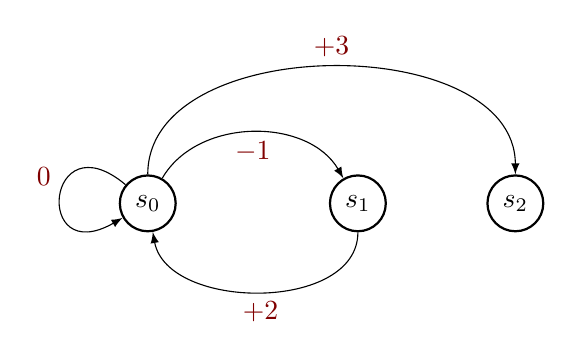
\begin{tikzpicture}[auto,node distance=58mm,>=latex]
    \tikzstyle{round}=[thick,draw=black,circle]
    \node[round] (s0) {$s_0$};
    \node[round, above=10mm, right=23mm] (s1) {$s_1$};
    \node[round, below=30mm, right=43mm] (s2) {$s_2$};

    \draw[->] (s0) [out=60,in=120] to node {} node [swap] {\textcolor{Maroon}{$-1$}} (s1);
    \draw[->] (s1) [out=-90,in=-80] to node {\textcolor{Maroon}{$+2$}} node [swap] {} (s0);
    \draw[->] (s0) [out=90,in=90] to node {\textcolor{Maroon}{$+3$}} node [swap] {} (s2);
    \draw[->] (s0) [out=140,in=210,loop] to node {} node [swap] {\textcolor{Maroon}{$0$}} (s0);




\end{tikzpicture}

\caption{A visual representation of a simple MDP. For each state transition the corresponding reward is presented in red.}
\label{fig:mdp}
\end{figure}

When dealing with MC learning, it can be possible that a certain state is visited more than once before a terminal state is reached. In the MDP represented in Fig. \ref{fig:mdp} this is the case for $s_0$. If that happens, one must decide when to update $V(s)$ and which value to use as $G_t$, as different state visits result in different $G_t$ values. There are two typical ways to deal with this: either update $V(s)$ only once, or one can update $V(s)$ each time the state is visited by simply using as $G_t$ the average of all the different discounted returns. 
While several successful applications of MC methods exist \cite{jaakkola1995reinforcement,liu1998sequential,lazaric2007reinforcement}, a well known issue from this family of algorithms is that they suffer from highly biased updates. In fact, one needs to compute the sum presented in Eq. \ref{eq:goal} over all visited states, resulting in returns with considerable variance. It is easy to see how this can become an issue, especially when the length of the episodes increases. In fact, the larger the episode's length, the more significant the variance of the updates. Furthermore, an additional drawback of MC methods is that one must wait until the agent visits a terminal state before being able to perform an update that is based on Eq. \ref{eq:mc_update}, a drawback that is addressed by the methods that are presented hereafter.   

\subsection{Temporal Difference Learning}
\label{sec:td_learning}
Temporal Difference (TD) Learning \cite{sutton1984temporal,sutton1988learning} is a learning paradigm that allows overcoming the issues mentioned above that characterize MC learning based methods. The key idea of TD-Learning is to update the value of each state with respect to a single MC update, therefore overcoming the hurdle of having to wait for the end of an episode before being able to update the value of a state. Just as MC methods TD-Learning algorithms also learn an optimal value function based on the experience that the agent collects. However, these algorithms base their updates only on the value of a single, consecutive state rather than on the real discounted return that is dependent on the entire sequence of visited states. Updating the value of a state with respect to the value of its successor state only is a technique that comes with the name of \textcolor{RoyalBlue}{bootstrapping}, and is a very effective design choice that reduces the variance in the updates. Bootstrapping can be used to learn the $V$ function and the $Q$ function and is at the core of the most popular model-free RL algorithms. The first and simplest form of TD-Learning was introduced by \citet{sutton1988learning} for learning the state-value function with an algorithm that updates the value of a state based on the following learning rule:
\begin{equation}
	V(s_t):= V(s_t) + \alpha \big[r_t + \gamma V(s_{t+1}) - V(s_t)\big].
	\label{eq:td_learning_v}
\end{equation}
We can now clearly see that differently from what happens in the MC update presented in Eq. \ref{eq:mc_update} the update of a state now only depends on the reward and the value of the next state. This quantity is denoted as the TD-error $\delta_t$ and is defined as:
\begin{equation}
	\delta_t = r_t + \gamma V(s_{t+1}) - V(s_t).
\end{equation}
where $r_t + \gamma V(s_{t+1})$ is also known as the TD-target.
If we again consider the simple MDP represented in Fig. \ref{fig:mdp} and assume that the value of each state of the process is set to $0$ while the discount factor $\gamma$ is this time set to $0.5$ and $\alpha$ is again $0.5$, a TD update for $V(s_0)$ based on a policy resulting in state $s_2$ will result into the new value estimate of $1.5$. 
TD-Learning is a very effective strategy for building algorithms that can learn in an online, fully incremental fashion as one only needs to wait for a single time-step before updating the considered value function. Due to its striking simplicity, TD-Learning has been widely adopted by RL practitioners developing algorithms for learning the $Q$ function. We will present some of the most important algorithms hereafter. 

\paragraph{\textbf{\uppercase{Q}-\uppercase{L}earning}} Introduced by \citet{watkins1992q} is arguably the most popular model-free RL algorithm. It works by keeping track of an estimate of the state-action value function $Q: \mathcal{S} \times \mathcal{A} \rightarrow \Re$ and updates each visited state-action pair with the following update rule:
\begin{equation}
Q(s_t,a_t):=Q(s_t,a_t) + \alpha\big[r_t + \gamma \:\underset{a\in \mathcal{A}}{\max} Q(s_{t+1},a_t) - Q(s_t, a_t) \big].
\label{eq:q_learning}
\end{equation}
The key component of Q-Learning's update rule is the $\max$ operator, which characterizes its TD-error and that is necessary for constructing the TD-target . Since there are as many Q values as there are actions available to the agent, one must choose which Q value to use as a reference when updating the value of the state-action pair that the agent is currently visiting. The $\max$ operator simply chooses the state-action pair with the largest Q value, a simple design choice that has the appealing property of making Q-Learning converge to $Q^{*}(s, a)$ with probability 1 as long as all state-action pairs are visited infinitely often. Interestingly, this guarantee holds even if the agent follows a random policy. The $\max$ operator also defines Q-Learning as an \textcolor{RoyalBlue}{off-policy} learning algorithm, since the Q values chosen for the construction of the TD-target might not correspond to the ones that are associated with the state that the agent will visit after having updated its $Q$ function.

\paragraph{\textbf{\uppercase{SARSA}}} Also known as "online Q-Learning" \cite{rummery1994line} can be seen as the most straightforward extension of the TD-Learning method presented in Eq. \ref{eq:td_learning_v}, and similarly to Q-Learning is an algorithm that aims at learning the state-action value function $Q$. The key idea of SARSA is to update a state-action value with respect to the Q value that is associated to the state that the agent will visit after a certain action is performed. Therefore, SARSA does not use the $\max$ operator within its TD-error and constructs TD-targets that represent the policy that the agent is following, a characteristic that defines SARSA as an \textcolor{RoyalBlue}{on-policy} RL algorithm. The way SARSA learns the $Q$ function is given by the following update rule
\begin{equation}
	Q(s_t,a_t):=Q(s_t,a_t) + \alpha\big[r_t + \gamma Q(s_{t+1},a_{t+1}) - Q(s_t, a_t) \big], 
	\label{eq:sarsa}
\end{equation}
where we can clearly see how the algorithm uses all the elements of the quintuple of events $(s_t, a_t, r_t, s_{t+1}, a_{t+1})$ a property that gives rise to the name $sarsa$. Not using the $\max$ operator in Eq. \ref{eq:sarsa} results in an algorithm that, differently from Q-Learning, does not directly learn the optimal $Q$ function anymore, but rather learns to estimate $Q^{\pi}(s,a)$. This has the drawback of not guaranteeing convergence to $Q^{*}(s,a)$ for any random policy anymore. To overcome this, SARSA needs an exploration policy that is greedy in the limit of infinite exploration \cite{singh2000convergence}. This can be achieved with the popular $\epsilon$-$\text{greedy}$ selection policy which defines the action that the agent takes as:
\begin{equation}
a_t = \begin{cases}
\underset{a\in\mathcal{A}}{\argmax} \ Q(s_t,a) &\text{with probability $1-\epsilon$}\\
a \sim \mathcal{U}(\mathcal{A}) &\text{with probability $\epsilon$}
\end{cases}
\label{eq:e_greedy}
\end{equation}
where $\epsilon$ is a hyperparameter that changes while training progresses. During early training iterations, its value is close to $1$, while it approaches $0$ by the end of training. This allows the agent to take actions that are representative of a large set of policies when the learned $Q$ function does not yet correspond to $Q^{*}(s,a)$, while it will favor greedy actions at the end of training. This is a simple, yet effective strategy that deals with the \textcolor{RoyalBlue}{exploration-exploitation} dilemma. It is however worth noting that its use is not limited to on-policy RL algorithms only. Furthermore, the method presented in Eq. \ref{eq:e_greedy} represents only one possible way of balancing exploration and exploitation, and although it is arguably the most popular of such methods, it is not the only existing one. We refer the reader to chapter 5 of \cite{wiering1999explorations} for a thorough analysis of different exploration algorithms.

\paragraph{\textbf{\uppercase{D}ouble \uppercase{Q}-\uppercase{L}earning}} In some environments, Q-Learning is known to perform poorly. This poor performance stems from the fact that the algorithm largely overestimates some state-action values due to the $\max$ operator in its TD-error \cite{thrun1993issues}. The $\max$ operator serves for constructing an approximation of the maximum expected action-value of a state, which, as discussed by \citet{hasselt2010double}, is a technique that results in positively biased estimates \cite{van2004rational,smith2006optimizer}. In some RL problems, this can significantly influence the learning process, which has led the RL community to develop a set of solutions that try to mitigate this bias \cite{lee2013bias,lee2019bias,zhu2020self,pentaliotis2021variation}. Among the different solutions, Double Q-Learning \cite{hasselt2010double} is probably the most popular one. Its main idea is to keep track of two different state-action value functions, $Q_1$ and $Q_2$, which get alternatively used for selecting which action to perform. When one of the two $Q$ functions determines the action that maximizes the state-action value of the next state, the remaining value function is used for evaluating this estimate. This can be achieved with the following rule:
\begin{equation}
	Q_1(s_t,a_t):=Q_1(s_t,a_t) + \alpha\big[r_t + \gamma \: Q_2(s_{t+1},a^{*}) - Q_1(s_t, a_t) \big],
\label{eq:double_q_learning}
\end{equation}
where $a^{*}=\argmax_{a\in \mathcal{A}} Q_1(s_{t+1},a)$. Note that at each time step, only one of the two $Q$ functions gets updated. While training progresses, the choice of which $Q$ function to update is determined randomly. In the case it is $Q_2$, the update rule is identical to the one presented in Eq. \ref{eq:double_q_learning} with the only difference being that the role of the two $Q$ functions is swapped. Double Q-Learning converges to the optimal state-action value function with probability $1$ under the same conditions as Q-Learning. \citet{hasselt2010double} shows that using two separate $Q$ functions significantly mitigates the overestimation bias. Yet, this comes at the price of an algorithm that is twice more expensive in terms of memory requirements. It is also worth noting that although Double Q-Learning does not overestimate the state-action values, it might instead underestimate them, which in some environments can still yield poor performance.


\paragraph{\textbf{\uppercase{QV}($\lambda$)-\uppercase{L}earning}} First introduced by \citet{wiering2005qv} and further developed by \citet{wiering2009qv} is an on-policy RL algorithm which differently from the previously introduced methods keeps track of an estimate of the state-value function $V:\mathcal{S}\rightarrow\mathbb{R}$ alongside the usual estimate of the state-action value function $Q:\mathcal{S}\times\mathcal{A}\rightarrow\mathbb{R}$. Since the goal is to jointly learn two value functions, QV($\lambda$)-Learning requires two separate update rules. The $V$ function is learned via the same form of TD-Learning that we introduced in Eq. \ref{eq:td_learning_v}, with the only difference being the addition of the eligibility traces $e_t(s)$ at the end of the update rule (an RL technique that we will review in Chapter \ref{ch:dqv_family_of_algorithms}). QV($\lambda$)-Learning, therefore, learns the $V$ function with the following update rule:
\begin{equation}
V(s):= V(s) + \alpha \big[ r_{t} + \gamma V(s_{t+1}) - V(s_t) \big] e_{t}(s).
\label{eqch02:qv_lambda_v_update}
\end{equation}
Since as discussed earlier only learning the $V$ function is not sufficient for deriving an optimal policy one needs to learn the $Q$ function as well. In QV($\lambda$)-Learning this is done as follows:
\begin{equation}
Q(s_{t}, a_{t}):= Q(s_{t}, a_{t}) + \alpha \big[r_{t} + \gamma V(s_{t+1}) - Q(s_{t}, a_{t}) \big].
\label{eqch02:qv_lambda_q_update}
\end{equation}
An attractive property of the algorithm is that it uses the same TD-target ($r_t + \gamma V(s_{t+1})$) for defining the two different TD-errors that are required for learning the state-value and the state-action value functions. Among the main insights that motivate learning two value functions over one, \citet{wiering2005qv} mentions the possibility that the $V$ function, since it does not depend on the agent's actions, might converge faster than the $Q$ function. As described earlier, the $V$ function only depends on the state space of the MDP, which by definition is smaller than the state-action space. For a more in-depth and formal presentation of the conditions that show the benefits of jointly learning the $V$ function alongside the $Q$ function, we refer the reader to chapter 5 of \cite{van2011insights}.


\section{Function Approximators}
\label{sec:function_approximators}
If it is true that model-free RL algorithms are very powerful methods for learning an optimal policy when parts of the MDP are unknown, it is also true that all the algorithms mentioned above suffer from the \textcolor{RoyalBlue}{curse of dimensionality}. Model-free algorithms are typically implemented in a tabular fashion, meaning that the state values, or state-action values, are stored within tables of sizes $|\mathcal{S}|$ and $|\mathcal{S}\times\mathcal{A}|$ respectively. Albeit straightforward and easy to implement, such an approach presents severe limitations. The first major drawback of the tabular representation approach is that it does not scale well with respect to the MDP complexity. If the environment state and action spaces become very large, storing a table quickly becomes unfeasible in terms of storage space. Furthermore, tabular representations are also unable to deal with continuous states. A natural solution to this problem could consist in discretizing the state space; however, this approach still results in the aforementioned storage space issues when done thoroughly. Therefore, if one wants to use RL techniques, even when the state space of the MDP is large, a better solution is needed. This solution is based on \textcolor{RoyalBlue}{parametrized function approximation}. In this context, the goal is not to learn the exact value function anymore but to rather replace its tabular representation with a parametrized function. This function parameters can then be adjusted based on the RL algorithms that we introduced in Sec. \ref{sec:td_learning}. 

\subsection{Linear Functions}
\label{sec:linear_functions}

The most straightforward type of function approximator one can use is a linear function. Given a state-action tuple that gets represented as a feature vector $\vec{x}(s)=[x_1(s), x_2(s), ..., x_q(s)] \in \mathds{R}^q$, and a function parametrized by a vector of parameters $\mathbold{\theta}^a\in\mathds{R}^q$ for each action $a\in\mathcal{A}$, as shown in \cite{wiering2004convergence}, we can redefine the value of a state-action pair as:
\begin{equation}
	Q(s,a) = \sum_i \theta^a_{i} x_i(s).
\end{equation}
Given a trajectory $\langle s_t,a_t,r_t,s_{t+1}\rangle$, the Q-Learning algorithm presented in Eq. \ref{eq:q_learning} can now be used for updating the parameters $\theta^a_i$ for all $i$ with the following update rule:
\begin{equation}
	\theta^{a_t}_{i} := \theta^{a_t}_{i} + \alpha(r_t +\gamma\:\underset{a\in \mathcal{A}}{\max} Q(s_{t+1},a_t) - Q(s_t, a_t)) x_i(s_t).
	\label{eq:q_learning_fa}
\end{equation}
We can observe that this update rule modifies the parameter vectors $\mathbold{\theta}^a$ by minimizing the mean squared error loss between a given state-action tuple and Q-Learning's TD-target since  
\begin{equation}
\begin{split}
	& \mathcal{L}(\theta) = \frac{1}{2}\big(y_t - Q(s_t, a_t)\big)^2 \mbox{ with } y_t = r_t +\gamma\:\underset{a\in \mathcal{A}}{\max} Q(s_{t+1},a_t) \\ 
	& \frac{\partial\mathcal{L}}{\partial \theta_{i,a_t}}=-\big(y_t - Q(s_t, a_t)\big) x_i(s_t)  \\ 
 	& \theta^{a_t}_{i} := \theta^{a_t}_{i} + \alpha(r_t +\gamma\:\underset{a\in \mathcal{A}}{\max} Q(s_{t+1},a_t) - Q(s_t, a_t)) x_i(s_t).
\end{split}
\end{equation}

Similar steps can be used for adapting all of the RL algorithms that we introduced in the previous section. As a representative example for the on-policy learning case let us consider the SARSA algorithm. One can learn an approximation of the $Q$ function by updating the parameters of a linear function as follows:

\begin{equation}
	\theta^{a_t}_{i} := \theta^{a_t}_{i} + \alpha(r_t +\gamma Q(s_{t+1},a_{t+1}) - Q(s_t, a_t)) x_i(s_t).
\end{equation}
Linear functions can yield successful results \cite{lane1992theory, park1993approximation, mcculloch1943logical} as they can indeed deal with the aforementioned curse of dimensionality problem. However, \textcolor{RoyalBlue}{non-linear} functions are usually preferred since their representational power is even larger than the one of linear methods. Throughout this dissertation, we are interested in non-linear functions that come in the form of deep neural networks. As we have seen in the previous chapter, neural networks such as e.g convolutional networks are able to learn very rich representations from their inputs. However, this also makes these kinds of models particularly challenging to train in an RL context. We will now describe how one can successfully deal with some of the challenges that characterize the use of deep neural networks in RL by presenting some of the most important algorithms that have been introduced over the years.    

\section{Deep Reinforcement Learning}
\label{sec:deep_reinforcement_learning}
Before looking into how RL algorithms should be integrated within deep neural networks, it is important to mention that RL techniques have been successfully combined with (less powerful) neural networks for over three decades. In fact, the field known as \textcolor{RoyalBlue}{Connectionist Reinforcement Learning} (CRL) resulted in the very first algorithms that managed to outperform human experts on specific tasks. Among the multiple possible examples of this family of techniques, we mention the TD-Gammon program introduced by \citet{tesauro1994td}. TD-Gammon successfully learns an approximation of the popular Backgammon boardgame's evaluation function through the same TD-Learning methods that we presented in Sec. \ref{sec:td_learning}. Tesauro's program achieved a level of play comparable to the one of the top human Backgammon players of its time and is even nowadays considered one of the most important RL breakthroughs. For a more detailed presentation about the successful applications of CRL algorithms, we refer the reader to \cite{bucsoniu2011approximate}.  

While certainly successful for a certain set of problems (see for example chapter $1$ of \cite{sabatelli2017learning}), CRL techniques also present severe limitations. Since they only use multi-layer perceptrons as function approximators, these algorithms cannot be used for tackling problems where the state representation of the MDP is highly dimensional. To overcome this, more complicated and powerful networks are required. \textcolor{RoyalBlue}{Deep Reinforcement Learning} (DRL) \cite{arulkumaran2017deep, li2017deep, franccois2018introduction} is a research field that combines RL algorithms with deeper and more complex neural architectures. In value based model-free DRL we are interested in learning an approximation of an optimal value function with a deep neural network that comes with parameters $\theta$

\noindent
\begin{tabularx}{\linewidth}{@{}XX@{}}
\begin{equation}
	  V(s;\theta)\approx V^{*}(s)
	  \label{eq:v_approx}
  \end{equation}
&
\begin{equation}  
	Q(s,a;\theta)\approx Q^{*}(s,a)
	\label{eq:q_approx}
  \end{equation}
\end{tabularx}
and that usually comes in the form of a convolutional neural network. We now describe some of the algorithms which have contributed to the development of DRL the most. 


\paragraph{\textbf{\uppercase{D}eep \uppercase{Q}-\uppercase{L}earning (\uppercase{DQN})}} Just like Q-Learning is arguably the most important tabular model-free RL algorithm, so is DQN when it comes to DRL. First introduced by \citet{mnih2013playing} and then made popular by the work presented in \cite{mnih2015human} this algorithm can certainly be considered as the very first successful example of a neural network that is able to learn an approximation of the optimal state-action value function just from high sensory inputs (in this case images). As the name suggests, Deep Q-Learning (DQN)\footnote{In DQN the `N" in the acronym stays for `Network" and replaces what could have been the, arguably more intuitive, `L" of Learning.} is based upon the Q-Learning algorithm and aims at learning an approximation of the optimal state-action value function $Q$. This is done by reshaping Q-Learning's update rule, presented in Eq. \ref{eq:q_learning}, into a differentiable loss function that can be used for training a convolutional network. This is achieved through the following objective function:
\begin{multline}
	\mathcal{L}(\theta) = \mathds{E}_{\langle s_{t},a_{t},r_{t},s_{t+1}\rangle\sim U(D)} \bigg[\big(r_{t} + \gamma \: \underset{a\in \mathcal{A}}{\max}\: Q(s_{t+1}, a; \theta^{-}) \\ - Q(s_{t}, a_{t}; \theta)\big)^{2}\bigg].
\label{eq:dqn}
\end{multline}

We can start by observing that the general principles that characterize the algorithm are the same ones that made it possible to generalize Q-Learning to the use of linear function approximators, however, differently from when a linear function is used, the mapping between input and feature spaces is now naturally not preserved anymore. Similarly to what we presented in Sec. \ref{sec:linear_functions}, we can see from Eq. \ref{eq:dqn} that learning $Q(s,a,\theta)$ is again achieved by minimizing the squared error loss between the $Q(s_t,a_t;\theta)$ estimates and the off-policy TD-target
\begin{equation}
    y^{DQN}_{t} = r_{t} + \gamma \: \underset{a\in \mathcal{A}}{\max}\: Q(s_{t+1}, a; \theta^{-}).
\label{eq:dqn_td}
\end{equation}
Despite this similarity, DQN requires some additional algorithmic design choices, without which it would turn out to be almost impossible to successfully train a neural network with Eq. \ref{eq:dqn}. These additions, which significantly make DQN differ from the algorithm presented in Eq. \ref{eq:q_learning_fa} are the following:
\begin{itemize}
	\item \textcolor{RoyalBlue}{Experience Replay}: a memory buffer, $D$, represented as a queue which stores RL trajectories of the form $\langle s_{t}$, $a_{t}$, $r_{t}$, $s_{t+1} \rangle$. Once this memory buffer is filled with a large set of these quadruples, DQN uniformly samples batches of trajectories for training its network. This makes it possible to exploit past trajectories multiple times by reusing them while training, which makes the overall algorithm more sample efficient. Furthermore, using a memory buffer also improves the stability of the training procedure. Recall that each trajectory is representative of a certain episode. By repeatedly randomly sampling a different $\tau$ from the memory buffer, a resulting mini-batch of trajectories will be representative of different episodes and of different policies. As a consequence, the correlation between trajectories within a mini-batch will be small. Although made popular by the DQN algorithm, using an experience replay buffer for tackling sequential decision making problems was already presented by \citet{lin1992self}.
		
	\item \textcolor{RoyalBlue}{Target Network}: We can observe from Eq. \ref{eq:dqn_td} that the TD-target used by DQN for bootstrapping is not computed by the $Q$ network that is being optimized ($\theta$), but rather from a second separate network that is parametrized with $\theta^{-}$. This second network has the same structure as the main $Q$ network, but its weights do not change each time RL experiences are sampled from $D$. On the contrary, its weights are temporally frozen and only periodically get updated with the parameters of the main network $\theta$ as defined by an appropriate hyperparameter. Note that this is a design choice that is not motivated by the TD-Learning paradigm that we presented in Sec. \ref{sec:td_learning}, where we have seen that TD-Learning based methods learn in a fully online fashion by updating their value estimates based on their own future estimates. With a target-network, although the $\theta$ network still learns via the methods of temporal differences, it now requires an auxiliary, external model if it wants to successfully learn $\approx Q^{*}(s,a;\theta)$. Several works have studied the target network's role to understand why this design choice appears to be necessary for DRL. Yet, the DRL community does not fully understand the role of $\theta^{-}$. For more about this topic, we refer the reader to \cite{kim2019deepmellow, piche2021beyond}.

\end{itemize}

With all these concepts in place we can show that given a training iteration $i$, differentiating this objective function with respect to $\theta$ gives the following gradient: 
\begin{multline}
\nabla_{\theta_{i}} \mathcal{L}(\theta_{i}) = \mathds{E}_{\langle s_{t},a_{t},r_{t},s_{t+1}\rangle\sim U(D)} \bigg[\big(r_{t} + \\ \gamma \: \underset{a\in \mathcal{A}}{\max}\: Q(s_{t+1}, a; \theta^{-}_{i-1})  - Q(s_{t}, a_{t}; \theta_{i})\big)\nabla_{\theta_{i}} Q(s_{t}, a_{t}; \theta_{i})\bigg].
\label{eq:dqn_gradient}
\end{multline}

The DQN algorithm showcased its entire potential in \cite{mnih2015human} where Mnih and colleagues developed a convolutional neural network that trained with Eq. \ref{eq:dqn} learned how to successfully play most of the \texttt{Atari} games that are part of the popular Atari Arcade Learning Environment (ALE) \cite{bellemare2013arcade}, a well-known platform that even nowadays serves as a benchmark for testing the performance of DRL algorithms. In the ALE, a DRL algorithm has to learn how to play $57$ different emulations of \texttt{Atari} games which are specifically designed within a simulator (see Fig. \ref{fig:atari_games} for a visualization of some of the games that are part of the ALE suite). Remarkably, DQN not only learned how to play most of the games of the platform but also achieved a final performance that, on most games, was superior to the one of human expert players. What is even more remarkable is that this was achieved by providing as inputs to the network the images representing the game only, therefore making the model learn just from its own experience in a pure model-free RL fashion. Since then, DQN has been successfully used for a large variety of applications ranging from healthcare \cite{tseng2017deep,raghu2017continuous}, robotics \cite{kalashnikov2018qt} and natural language processing \cite{he2015deep, narasimhan2015language} to even particle physics \cite{liu2017learning, sajedian2020design}. However, despite all these remarkable applications, the algorithm still comes with some drawbacks, some of which are addressed by the algorithms presented below.

\begin{figure}[ht!]
\centering
  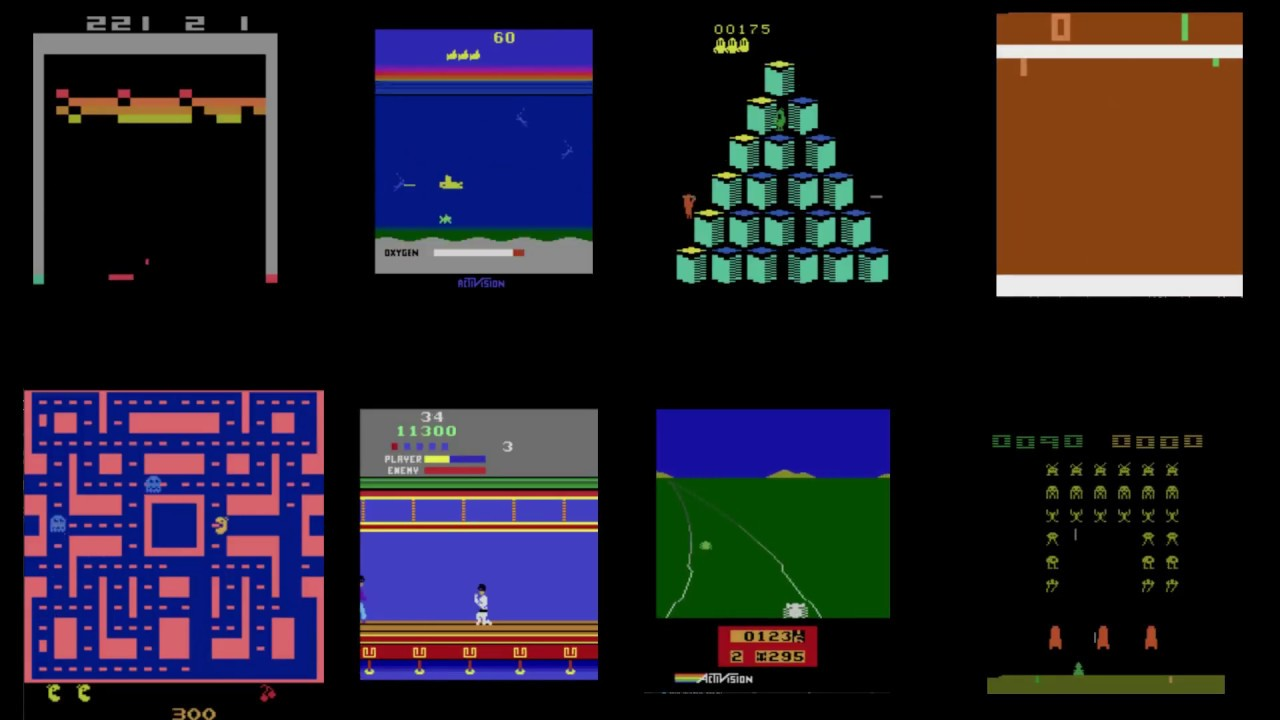
\includegraphics[width=10cm]{./Images/Chapter02/atari_games}
  \caption{A visual representation of some of the \texttt{Atari} games that are part of the Arcade Learning Environment (ALE) \cite{bellemare2013arcade}. From left to right \texttt{Breakout, Seaquest, Qbert, Pong, MsPacman, KungFu-Master, Enduro} and \texttt{Space Invaders}. Most of these games will be of interest in Chapter \ref{ch:dqv_family_of_algorithms} and Chapter \ref{ch:dqn_transfer}.}
  \label{fig:atari_games}
\end{figure}


\paragraph{\textbf{\uppercase{D}ouble \uppercase{D}eep \uppercase{Q}-\uppercase{L}earning (\uppercase{DDQN})}} \citet{van2016deep} showed that the DQN algorithm suffers from the same issue that also characterizes the Q-Learning algorithm: the overestimation bias of the $Q$ function. They show that DQN is prone to learn overestimated Q-values because the same values are used both for selecting an action ($\underset{a\in \mathcal{A}}{\max}$) as well as for evaluating it ($Q(s_{t+1},a;\theta^{-})$). This becomes clearer when re-writing DQN's TD-target presented in Eq. \ref{eq:dqn_td} as:
\begin{equation}
    y^{DQN}_{t} = r_{t} + \gamma \: Q(s_{t+1}, \underset{a\in \mathcal{A}}{\argmax}\: Q(s_{t+1}, a; \theta); \theta^{-}). 
\end{equation}{}
As a result, DQN tends to approximate the expected maximum value of a state, instead of its maximum expected value. As presented in Sec. \ref{sec:td_learning}, in the tabular case this can be solved by keeping track of two separate $Q$ functions, and by randomly preferring one $Q$ function over the other when it comes to selecting which action to execute. DDQN generalizes this idea and untangles the action selection process from its evaluation by taking advantage of the previously introduced target network $\theta^{-}$. DDQN's target stays the same as in DQN with the main difference being that the selection of an action, given by the online Q-network $\theta$, and the evaluation of the resulting policy, given by $\theta^{-}$, can now result into smaller overestimations simply by symmetrically updating the two sets of weights ($\theta$ and $\theta^{-}$) which can easily be achieved by regularly switching their roles during training. While not always significantly impacting the performance of DQN (one can still act optimally even if some actions are associated to unrealistically high $Q(s,a)$ estimates), there are also cases for which the overestimation bias of the $Q$ function significantly slows down the training process, and even prevents the DQN algorithm from improving its policy over time at all. We will come back to this issue in Chapter \ref{ch:dqv_family_of_algorithms}. 


\paragraph{\textbf{\uppercase{P}rioritized \uppercase{E}xperience \uppercase{R}eplay (\uppercase{PER})}} We have seen that next to the target network $\theta^{-}$ an equally important role within the DQN algorithm is played by the experience replay memory buffer $D$. \citet{schaul2015prioritized} showed that the efficiency of how Deep Q-Networks use this buffer could be improved. Their claim stems from the fact that, as shown in Eq. \ref{eq:dqn}, the RL trajectories that get sampled from the memory buffer when constructing a mini-batch of trajectories are sampled uniformly ($\sim U(D)$). This approach has the main drawback that it considers each $\tau$ stored in the buffer as equally important and representative for training. However, it is easy to imagine learning situations where some trajectories are more valuable than others. For example, at the beginning of training, most of the trajectories contained within $D$ will be representative of early agent-environment interactions. It is, therefore, safe to assume that the network will learn the $Q(s,a)$ estimates representative of these early dynamics much faster than it will learn the $Q$ values that are associated with trajectories occurring more rarely. The idea of PER is to use only highly informative trajectories when it comes to building the mini-batches that are used for training the network. The importance of different trajectories is given by their respective TD-error. PER ensures that the probability of sampling trajectories is proportional to their respective TD-errors: the higher the TD-error, the larger the probability for a specific $\tau$ to be sampled. In practice, given a trajectory $\tau$, the probability of sampling it is given by the following equation:
\begin{equation}
	P(\tau)=\frac{p_{\tau}^{\alpha}}{\sum_k p_{k}^{\alpha}}
\end{equation}
where $p_{\tau}$ is $|\delta_\tau + \epsilon|$ with $\epsilon$ being a small positive number ensuring that the probability of sampling a trajectory remains positive even in the edge case where the TD-error is $0$. Although simple and intuitive, implementing a PER buffer is not that straightforward and still presents some algorithmic caveats that need to be taken into account. Yet, if done correctly it dramatically improves the sample efficiency of Deep Q-Networks \cite{narasimhan2015language}.

\paragraph{\textbf{\uppercase{D}ueling \uppercase{N}etworks}} While the DDQN algorithm directly tackles a fundamental algorithmic bias that characterizes the way DQN learns the $Q$ function, and PER addresses the inefficiency of its memory buffer, the contribution presented by \citet{wang2016dueling} is of slightly different nature. Their work consists of a novel type of neural architecture called the Dueling Network. This is a contribution that resembles more the kind of progress that is made by the supervised learning community, which, as we discussed in the previous chapter, has put a lot of effort into developing novel neural architectures for tackling computer vision tasks. Nevertheless, Wang's work is a perfect example that showcases how in DRL, carefully designing the function approximator is just as important as properly defining its objective function. A Dueling network is a network that, after performing a series of convolutions, instead of directly outputting the state-action values for a specific state as DQN and DDQN do, adds some intermediate computations. The idea is to estimate the value of a state and the advantages for each action before outputting the final $Q$ values. The state values are computed based on Eq. \ref{eq:state_value_function}, while the advantage function $A$ is simply the difference between the $Q$ function and the $V$ function:
\begin{equation}
	A^{\pi}(s,a) = Q^{\pi}(s,a) - V^{\pi}(s).
\end{equation}
To successfully estimate state values, advantages, and state-action values, the network requires a specific architecture consisting of three separate streams. Each stream is responsible for estimating one of the three value functions and is initialized with its own parameters $\theta^{(\cdot)}$. The final $Q$ function of the model is then obtained by combining what is learned by each stream as follows:
\begin{multline}
	Q(s,a;\theta^{(1)},\theta^{(2)},\theta^{(3)}) = V\bigl(s;\theta^{(1)},\theta^{(3)}\bigr) + \\
	\bigl(A(s,a;\theta^{(1)},\theta^{(2)}) - \underset{a_{t+1}\in \mathcal{A}}{\max}\: A(s, a_{t+1};\theta^{(1)},\theta^{(2)}) \bigr).
	\label{eq:dueling}
\end{multline}
Building a network with different task-specific streams is a design choice that resembles the way models are built when tackling multitask classification tasks. However, note that the output of each stream that either estimates the state values or the advantage function gets aggregated in a final layer that estimates the state-action values. Training a Dueling Network is done by minimizing the same objective function that is also minimized by DQN and DDQN. The idea of taking into account the $V$ function when learning the $Q$ function is a concept which will come back, in a different flavor, in Chapter \ref{ch:dqv_family_of_algorithms} and Chapter \ref{ch:dqn_transfer}.

\paragraph{\textbf{\uppercase{P}olicy \uppercase{G}radient \uppercase{M}ethods}} So far we have only considered algorithms that are part of the action-value family of methods, which, as explained in Sec. \ref{sec:learning_value_functions} are techniques that derive an optimal policy from a learned $Q$ function. Yet, there is a collection of algorithms that is able to learn a policy directly, and that therefore bypasses the requirement of having to consult state-action values when it comes to action selection. These methods, which have contributed to the development of DRL just as much as action-value methods, come with the name of Policy Gradients. They directly parametrize a policy at each time-step as $\pi(a|s;\theta)=\text{Pr}\:\{a_t = a| s_t=s;\theta_t=\theta\}$ and seek to optimize the parameters $\theta$ such that the performance of the policy is maximized. Note that this is drastically different from all the methods which we have seen so far, where the aim, in fact, was to minimize the TD-error through gradient descent optimization. Since policy gradients aim to maximize their performance, they learn via gradient ascent and therefore update their parameters as follows
\begin{equation}
	\theta \leftarrow \theta + \alpha \nabla \xi(\theta).
\end{equation}
Here $\alpha$ is again the learning rate, and $\xi$ is a measure that quantifies the performance of the policy. Similarly to action-value based methods, one can parametrize a policy either with a linear function or with a deep neural network. When the action space is discrete, it is common practice to parametrize $\pi$ through the same exponential softmax distribution, which we have seen in the previous chapter when presenting neural networks trained for classification tasks. Therefore we have
\begin{equation}
	\pi(a|s;\theta) = \frac{e^{h(s,a;\theta)}}{\sum_b e^{h(s,b;\theta)}}
\end{equation}
where $h(s,a;\theta)$ is any function approximator. By doing so, policy gradient methods naturally deal with the exploration-exploitation trade-off since they simply assign different probabilities to different actions. This also allows these methods to approach a deterministic policy (which cannot be achieved when using $\epsilon$-greedy action selection) and makes these algorithms arguably easier to train since learning a policy could be easier than learning state-action returns. The fundamental result which allows optimizing any differentiable policy is the policy gradient theorem \cite{sutton1999policy}. \citet{sutton1999policy} show that the gradient of $\pi$ does not depend on the gradient of the state distribution and that it can therefore be expressed as follows:
\begin{equation}
	\nabla \xi(\theta) = \sum_{s} \mu(s) \sum_{a} Q^{\pi}(s,a) \nabla \pi(a|s;\theta)
\end{equation}
where $\mu(s)$ is the stationary on-policy distribution under $\pi$. By expressing the gradient as such, it is now possible to optimize $\pi$ even when the state distribution of the environment is unknown (as discussed in Sec. \ref{sec:learning_value_functions}). Policy gradient methods can be used for learning a policy through the same kind of techniques which in Sec. \ref{sec:learning_value_functions} were used for learning value functions. Within the Monte Carlo setting the arguably most important of such algorithms is REINFORCE \cite{williams1992simple}, while Actor-Critic algorithms \cite{lillicrap2015continuous,schulman2015high,schulman2015trust,wang2016sample,mnih2016asynchronous,schulman2017proximal,haarnoja2018soft,fujimoto2018addressing} learn a policy with the additional help of a bootstrapped value function (typically $V$ or $A$).


\paragraph{\textbf{\uppercase{R}ainbow}} From the examples above, it is clear that much progress has been achieved by the DRL community in creating algorithms capable of learning faster and better. Explaining all the individual value-based contributions that have made DRL the popular research field it is nowadays \cite{henderson2018deep}, is beyond the scope of this chapter. Yet, if there is one algorithm that encapsulates most of the progress that the DRL community has achieved over the last years, that is Rainbow \cite{hessel2018rainbow}. Rainbow is a single, almighty agent that integrates most of the important breakthroughs that DRL researchers have introduced over the last decade within the same algorithm, ranging from the previously mentioned DDQN algorithm and PER system to more recent techniques such as distributional DRL \cite{bellemare2017distributional}, multi-step learning, distributed training \cite{mnih2016asynchronous} and noisy networks \cite{fortunato2017noisy} that allow for better exploration.


\section{The Deadly Triad of Deep Reinforcement Learning}
\label{sec:challenges}
We now end this chapter by presenting one of the main limitations that currently characterizes the field of DRL and that has inspired part of the research that is presented in this dissertation.

The combination of RL with function approximation can result in unstable training and algorithms prone to diverge while learning. As a representative example of what it means for an RL algorithm to diverge, let us consider the following MDP firstly introduced by \citet{tsitsiklis1997analysis}. The MDP consists of three states $s_0, s_1$ and the terminal state $s_2$. Each state is described by a single scalar feature $\psi$ such that $\psi(s_0)=1$ and $\psi(s_1)=2$. The estimated state-value of each state is therefore given by $V(s)=\psi \times w$, where $w$ is the single weight we would like to update. The MDP is represented in Fig \ref{fig:deadly_triad}.  
\begin{figure}[ht!]
	\centering
	\tikzset{
    ->, 
    level distance = 22em,
    minimum size=2em,
    %edge from parent/.style={draw,thick},
    level 1/.style={sibling distance=6em},
    level 2/.style={sibling distance=3em},
    thick/.style = {line width=1.5pt},
    extra thick/.style = {line width=3.5pt},
    red node/.style={shape=circle,draw=red,fill=red!40,thick,inner sep=1.2},
    blue node/.style={shape=circle,draw=blue,fill=blue!40,thick,inner sep=1.2}
}

\tikzstyle{round}=[thick,draw=black,circle]

\begin{tikzpicture}[auto,node distance=58mm,>=latex]
    \tikzstyle{round}=[thick,draw=black,circle]
    \node[round, label=below:$s_0$] (s0) {$w$};
    \node[round, label=below:$s_1$, above=10mm, right=23mm] (s1) {$2w$};
    \node[round, label=below:$s_2$, below=30mm, right=43mm] (s2);

    \draw (s0) -> (s1);
    \draw [->] (s1.90) arc (0:264:4mm); 
    \draw (s1) -> (s2);

    \path [line] (s1.90) -- node [text width=1.5cm,midway,above,align=center] {$1-\epsilon$} arc (0:264:4mm);

    \path [line] (s1) -- node [text width=2.5cm,midway,above,align=center ] {$\epsilon$} (s2);

\end{tikzpicture}

\caption{A visual representation of the MDP proposed by \citet{tsitsiklis1997analysis} that shows how RL algorithms combined with function approximators can diverge.}
\label{fig:deadly_triad}
\end{figure}
Each state transition is associated with a reward of $0$, which means that the optimal weight value for having perfect value predictions is $w^{*}=0$. Let us now assume that we are updating the state-value function based on an on-policy learning scheme as discussed in Sec. \ref{sec:td_learning}. We then know that each time we are updating the state-value function for $s_0$, the value of $s_1$ will, in expectation, also be updated multiple times. This however, changes if we are following an off-policy learning scheme since each time we update the state-value function for $s_0$, we do not necessarily update the value of $s_1$ anymore. As shown by \citet{van2018deep_triad} if we would now update $w$ based on Eq. \ref{eq:td_learning_v} we would have to modify $w$ as $\Delta w \propto r_t +\gamma(V(s_{t+1})-V(s_t))$. Which results into $0+\gamma 2w-w=\gamma 2w-w=(2\gamma-1)w$. If we then set the discount factor $\gamma>0.5$ as is common practice, we can see that we have $2\gamma>1$, which will make any weight $w\neq0$  be updated away from the desired value of $0$. \citet{sutton2018reinforcement} show that the cause of this type of divergence occurs when RL algorithms are combined with three concepts which we have already encountered in this chapter. These concepts are: bootstrapping (Sec. \ref{sec:td_learning}), off-policy learning (Sec. \ref{sec:td_learning}) and function approximation (Sec. \ref{sec:function_approximators}).
This combination is known as the `Deadly Triad" of DRL, and it is well known that if all of these three elements are combined within the same algorithm, divergence can appear. Divergence results in algorithms that are extremely slow to train, or even in agents that are not able to improve their policy over time at all. Throughout this dissertation we will tackle the problem of the Deadly Triad by first introducing novel algorithms that are less prone to diverge (Chapter \ref{ch:dqv_family_of_algorithms}), while in a second approach by investigating whether the particularly long training times that characterize such algorithms can be reduced by adapting transfer learning strategies (Chapter \ref{ch:dqn_transfer}).   




 % Reinforcement Learning + Deep Learning
\chapter{Transfer Learning from the Natural to the Non-Natural Domain}
\label{ch:tl_natural_to_non_natural}

\begin{remark}{Contributions and Outline} 
	This chapter contributes to the field of (Deep) Transfer Learning (TL) by investigating whether popular neural networks that come as pre-trained on datasets containing natural images can perform equally well once they are used on non-natural datasets. Specifically, we explore whether these models can be used for tackling three different art classification problems. Furthermore, assuming this is the case, we also explore whether it is possible to improve on such performance. The chapter is structured as follows: we start by providing the reader with some background information in Section \ref{sec:introduction}. In Section \ref{sec:methods} we present a brief theoretical reminder of the field of TL, a description of the datasets that we have used and the methodological details about the experiments that we have performed. In Section \ref{sec:results} we present and discuss our results. A summary of the main contributions of this work ends the chapter in Section \ref{sec:conclusion}.

\vspace{5mm}

\textit{This chapter is based on the publication \citet{sabatelli2018deep}.}
\end{remark}


% ---- Section 1 ----
\section{Introduction and Related Work}
\label{sec:introduction}

Over the past decade Deep Convolutional Neural Networks (DCNNs) have become one of the most used and successful algorithms in Computer Vision (CV) \cite{donahue2014decaf, ma2015multimodal,tome2016deep}. Due to their ability to automatically learn representative features by incrementally down sampling the input via a set of non linear transformations, these kind of neural networks have rapidly established themselves as the state of the art algorithm on a large set of CV problems. Within different CV testbeds large attention has been paid to the ImageNet challenge \cite{deng2009imagenet}, a CV benchmark that aims to test the performance of different image classifiers on a dataset that contains one million natural images distributed over thousand different classes. The availability of such a large dataset, combined with the possibility of training deep neural networks in parallel over several \texttt{GPUs} \cite{krizhevsky2012imagenet}, has lead to the development of a large set of different neural architectures that have continued to outperform each other over the years \cite{simonyan2014very,szegedy2016rethinking,chollet2016xception,he2016deep,huang2017densely}.     
A promising research field in which the classification performances of such DCNNs can be exploited is that of \textit{Digital Heritage} \cite{parry2005digital}. Due to a growing and rapid process of digitization, museums have started to digitize large parts of their cultural heritage collections, leading to the creation of several digital open datasets \cite{allen2000collaboration, mensink2014rijksmuseum}. The images constituting these datasets are mostly matched with descriptive metadata  which, as presented in e.g. \cite{mensink2014rijksmuseum}, can be used to define a set of challenging machine learning tasks. However, the number of samples in these datasets is far smaller than those in, for instance, the ImageNet challenge and this can become a serious constraint when trying to successfully train DCNNs from scratch.

The lack of available training data is a well known issue in the deep learning community and is one of the main reasons that has led to the development of the research field of Transfer Learning (TL). The main idea of TL consists of training a machine learning algorithm on a new task (e.g. a classification problem) while exploiting knowledge that the algorithm has already learned on a previously related task (a different classification problem). This machine learning paradigm has proved to be extremely successful in deep learning, where it has been shown how popular models that were trained on many large datasets \cite{huang2007labeled, stallkamp2011german}, were able to achieve very promising results on classification problems from heterogeneous domains, ranging from medical imaging \cite{tajbakhsh2016convolutional} or gender recognition \cite{van2015deep} over plant classification \cite{reyes2015fine} to galaxy detection \cite{ackermann2018using}.      

In this work we explore whether the TL paradigm can be successfully applied to three different art classification problems. We use four neural architectures that have obtained strong results on the ImageNet challenge in recent years and we investigate their performance when it comes to attributing the \textit{authorship} to different artworks, recognizing the \textit{material} which has been used by the artists in their creations, and identifying the \textit{artistic category} these artworks fall into. We do so by comparing two possible approaches that can be used to tackle the different classification tasks. The first one, known as off the shelf classification \cite{razavian2014cnn}, simply retrieves the features that were learned by the networks on other datasets and uses them as input for a new classifier. In this scenario the weights of the model do not change during the training phase, and the final, top-layer classifier is the only component of the architecture which is actually trained. This changes in our second explored approach, known as fine tuning, where the weights of the original network are ``unfrozen'' and the neural architectures are trained together with the final classifier. 

\citet{kornblith2018better} have shown the benefits that this particular pre-training approach has. In particular, DCNNs which have been trained on the ImageNet challenge typically lead to superior results when compared to the same architectures trained from scratch. However, this is not necessarily beneficial and in some cases networks that are randomly initialized are able to achieve the same performance as ImageNet pre-trained models. However, none of the results presented in \cite{kornblith2018better} report experiments on datasets containing heritage objects, it is thus still an open question how such pre-trained DCNNs would perform in such a classification scenario. In the rest of this chapter we report results that extensively study the performance of such neural networks; at the same time we also assess whether better TL performance can be obtained when using neural networks that, in addition to the ImageNet dataset, have additionally been pre-trained on a large artistic collection.  


\section{Methods}
\label{sec:methods}

We now present the methods that underpin our research. We start by giving a brief formal reminder of TL. We then introduce the three classification tasks under scrutiny, together with a brief description of the datasets. Finally, we present the neural architectures that we have used for our experiments. 

\subsection{Transfer Learning}
\label{subsec: tl}

A supervised learning (SL) problem can be identified by three elements: an input space ${\cal X}_t$, an output space ${\cal Y}_t$, and a probability distribution $p_t(x,y)$ defined over ${\cal X}_t\times {\cal Y}_t$ (where $t$ stands for 'target', as this is the main problem we would like to solve). The goal of SL is then to build a function $f:{\cal X}_t\rightarrow{\cal Y}_t$ that minimizes the expectation over $p_t(x,y)$ of a given loss function $\ell$ assessing the predictions made by $f$:
\begin{equation}\label{loss}
  E_{(x,y)\sim p_t(x,y)} \{\ell(y,f(x))\},
\end{equation}
when the only information available to build this function is a learning sample of input-output pairs $LS_t=\{(x_i,y_i)|i=1,\ldots,N_t\}$ drawn independently from $p_t(x,y)$. In the general transfer learning setting, one assumes that an additional dataset $LS_s$, called the source data, is available that corresponds to a different, but related, SL problem. More formally, the source SL problem is assumed to be defined through a triplet $({\cal X}_s,{\cal Y}_s,p_s(x,y))$, where at least either ${\cal X}_s\neq {\cal X}_t$, ${\cal Y}_s\neq {\cal Y}_t$, or $p_s\neq p_t$. The goal of TL is then to exploit the source data $LS_s$ together with the target data $LS_t$ to potentially find a better model $f$ in terms of the expected loss (\ref{loss}) than when only $LS_t$ is used for training this model. Transfer learning is especially useful when there is a lot of source data, whereas target data is more scarce.

Depending on the availability of labels in the target and source data and on how the source and target problems differ, one can distinguish different TL settings \cite{pan2010survey}. In what follows, we assume that labels are available in both the source and target data and that the input spaces ${\cal X}_t$ and ${\cal X}_s$, that both correspond to color images, match. Output spaces and joint distributions will however differ between the source and target problems, as they will typically correspond to different classification problems (ImageNet object recognition versus art classification tasks). Our problem is thus an instance of \textit{inductive transfer learning} \cite{pan2010survey}. While several inductive transfer learning algorithms exist, hereafter we focus on model transfer techniques, where information between the source and target problems is exchanged in the form of a neural network that comes as pre-trained on the source data. Although potentially suboptimal, this approach has the advantage of being more computationally efficient, as it does not require to train a model using both the source and the target data.


\subsection{Datasets and Classification Challenges}
\label{subsec:datasets}

For our experiments we use two datasets which come from two different heritage collections. The first one contains the largest number of samples and comes from the Rijksmuseum in Amsterdam\footnote{\url{https://staff.fnwi.uva.nl/t.e.j.mensink/uva12/rijks/}}. On the other hand, our second `Antwerp' dataset is much smaller. This dataset presents a random sample that is available as open data from a larger heritage repository: DAMS (Digital Asset Management System)\footnote{\url{https://dams.antwerpen.be/}}. This repository can be searched manually via the web-interface or queried via a Linked Open Data API. It aggregates the digital collections of the foremost GLAM institutions  (Galleries, Libraries, Archives, Museums) in the city of Antwerp in Belgium. Thus, this dataset presents a varied and representative sample of the sort of heritage data that is nowadays being collected at the level of individual cities across the globe. While it is much smaller, its coverage of cultural production is similar to that of the Rijksmuseum dataset and presents an ideal testing ground for the transfer learning task under scrutiny here.

Both image datasets come with metadata encoded in the Dublin Core metadata standard \cite{weibel1998dublin}. We selected three well-understood classification challenges: (1) ``material classification'' which consists in identifying the material the different heritage objects are made of (e.g paper, gold, porcelain, ...) ;  (2) ``type classification'' in which the neural networks have to classify in which artistic category the samples fall into (e.g. print, sculpture, drawing, ...), and finally (3) ``artist classification'', where the main goal is to appropriately match each sample of the dataset with its creator (from now on we refer to these classification tasks as challenge 1, 2 and 3 respectively). As reported in Table \ref{table:dataset_overview} we can see that the Rijksmuseum collection is the dataset with the largest amount of samples per challenge ($N_t$) and the highest amount of labels to classify ($Q_t$). Furthermore it is also worth noting that there was no metadata available when it comes to the first classification challenge for the Antwerp dataset (as marked by the $\times$ symbol), and that there are some common labels between the two heritage collections when it comes to challenge 2. A visualization reporting some of the images that are present in both datasets is shown in Figure \ref{fig:datasets}.


\begin{table}[ht!]
\scriptsize
\centering
\caption{An overview of the two datasets that are used in our experiments. Each color of the table corresponds to a different classification challenge, starting from challenge $1$ which is represented in yellow, challenge $2$ in blue and finally challenge $3$ in red. 
Furthermore we represent with $N_t$ the amount of samples constituting the datasets and with $Q_t$ the number of labels. Lastly, we also report if there are common labels between the two heritage collections.}
\begin{tabular}{c|c|c|c|c} 
	\hline
        Challenge & Dataset & \textbf{$N_t$} & \textbf{$Q_t$} & $\%$ of overlap \\\hline
        Material & Rijksmuseum  & $110,668$ & $206$ & None \\ 
         & Antwerp & $\times$ & $\times$    \\
        Type & Rijksmuseum  & $112,012$ & $1,054$   \\
         & Antwerp & $23,797$ & $920$ & $\approx 15\%$ \\
        Artist & Rijksmuseum & $82,018$ & $1,196$  & None \\ 
         & Antwerp  & $18,656$ & $903$ \\        
	\hline
\end{tabular}
\label{table:dataset_overview}
\end{table}   



\begin{figure}
\centering
  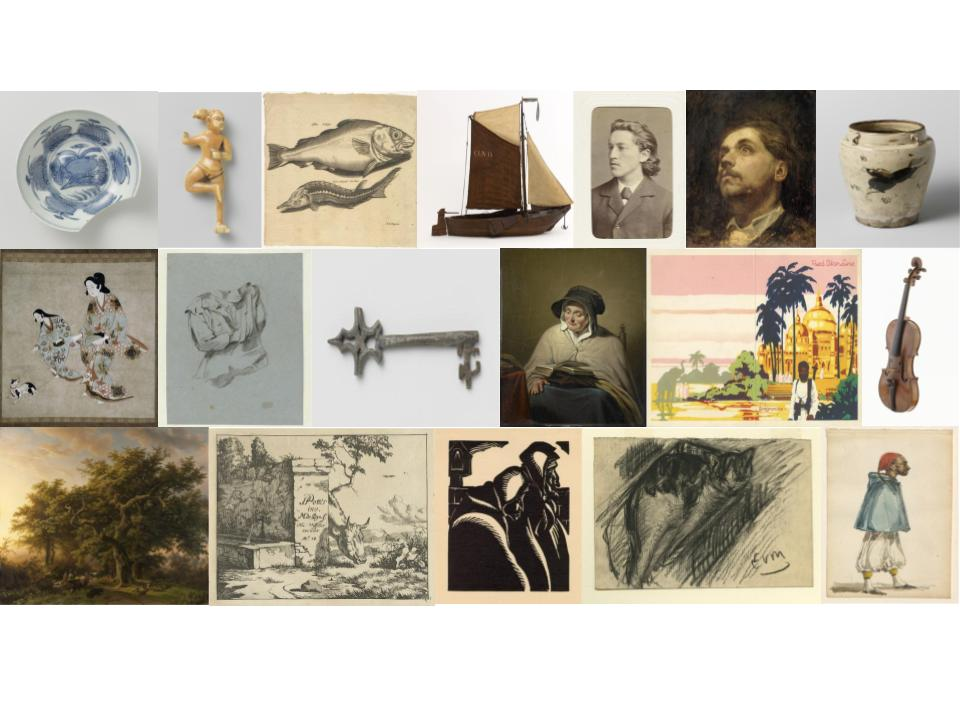
\includegraphics[width=10cm]{./Images/Chapter03/datasets.jpg}\vspace{-1cm}
  \caption{A visualization of the images that are used for our experiments. It is possible to see how the samples range from images representing plates made of porcelain to violins, and from Japanese artworks to a more simple picture of a key.}
  \label{fig:datasets}
\end{figure}

We use $80\%$ of the datasets for training while the remaining 2 x $10\%$ is used for validation and testing respectively. Furthermore, we ensure that only classes which occur at least once in all the splits are used for our experiments. Naturally, in order to keep all comparisons fair between neural architectures and different TL approaches, all experiments have been performed on the exact same data splits which, together with the code used for all our experiments, are publicly released to the CV community \footnote{\url{https://github.com/paintception/Deep-Transfer-Learning-for-Art-Classification-Problems}}. 

\subsection{Neural Architectures and Classification Approaches}
\label{subsec: neural_nets}

For our experiments we use four pre-trained DCNNs that have all obtained state of the art results on the ImageNet classification challenge. The neural architectures are VGG19 \cite{simonyan2014very}, Inception-V3 \cite{szegedy2016rethinking}, Xception \cite{chollet2016xception} and ResNet50 \cite{xie2017aggregated}. We use the implementations of the networks that are provided by the \texttt{Keras} Deep Learning library \cite{chollet2015keras} together with their appropriate \texttt{Tensorflow} weights \cite{abadi2016tensorflow} that come from the \texttt{Keras} official repository as well. Since all architectures have been built in order to deal with the ImageNet dataset we replace the final classification layer of each network with a new one. This final layer simply consists of a new \textit{softmax} output, with as many neurons as there are classes to classify, which follows a 2D global average pooling operation. We rely on this dimensionality reduction step because we do not add any fully connected layers between the last convolution layer and the \textit{softmax} output. Hence, in this way we are able to obtain a feature vector, $\mathscr{X}$, out of the rectified activation feature maps of the network that can be properly classified. Since all experiments are treated as a multi-class classification problem all networks minimize the \textit{categorical crossentropy} function loss function.

We investigate two possible classification approaches that are based on the previously mentioned pre-trained architectures. The first one, denoted as off the shelf classification, only trains a final \textit{softmax} classifier on $\mathscr{X}$, which is retrieved from the different models after performing one forward pass of the image through the network \footnote{Please note that instead of a \textit{softmax} layer any kind of machine learning classifier can be used instead. We experimented with both Support Vector Machines (SVMs) and Random Forests but since the results did not significantly differ between classifiers we decided to not include them here.}. This approach is intended to explore whether the features that are learned by the network on the ImageNet dataset are informative enough in order to properly train a machine learning classifier on the previously introduced art classification challenges. If this would be the case, such pre-trained models could be used as appropriate feature extractors without having to rely on expensive \texttt{GPU} computations for training. Naturally, they would only require the training of the final classifier without having to compute any backpropagation operations over the entire network. 

Our second approach is generally known as fine tuning and differs from the previous one by the fact that together with the final \textit{softmax} output the entire network is trained as well. This means that unlike the off the shelf approach, the entirety of the neural architecture gets ``unfrozen'' and is optimized during training. The potential benefit of this approach lies in the fact that the models get independently trained on samples coming from the artistic datasets, and therefore their classification predictions will not be restricted to what the networks previously learned on the ImageNet dataset only. Evidently, such an approach is computationally more demanding.

In order to maximize the performance of all models we follow some of the recommendations presented by \citet{masters2018revisiting} and train the networks with a relatively small batch size of $32$ samples. We do not perform any data augmentation operations besides a standard pixel normalization to the $[0, 1]$ range and a re-scaling operation which resizes the images to the input size that is required by the different models. Regarding the stochastic optimization procedures of the different classifiers, we use two different optimizers, that after preliminary experiments, turned out to be the best performing ones. For the off the shelf approach we use the RMSprop optimizer \cite{tieleman2012lecture} which has been initialized with its default hyperparameters (learning rate = $0.001$, a \textit{momentum} value $\rho = 0.9$ and $\epsilon =1e-08$). On the other hand, when we fine tune the DCNNs we use the standard (and less greedy) Stochastic Gradient Descent (SGD) algorithm with the same learning rate, $0.001$, and a \textit{Nesterov Momentum} value set to $0.9$.
Training has been controlled by the \textit{Early Stopping} method \cite{caruana2001overfitting} which interrupted training as soon as the validation loss did not decrease for $7$ epochs in a row. The model which is then used on the testing set is the one which obtained the smallest validation loss while training.

To the best of our knowledge, the results presented in this chapter are the first ones that systematically asses to which extent models pre-trained on the ImageNet dataset can be used as valuable architectures when tackling art classification problems. Furthermore, we also present the first results that investigate it is also not known whether the fine tuning approach can yield better results than the off the shelf one, and if using such pre-trained models would yield better performance than training the same architectures from scratch as observed by \citet{kornblith2018better}.

% END METHODS
%==================================================================================================================
% BEGIN RESULTS

\section{Results}
\label{sec:results}

Our experimental results are divided in two different sections, depending on which kind of dataset has been used. We first report the results that we have obtained when using architectures that were pre-trained on the ImageNet dataset only, and aimed to tackle the three classification problems of the Rijksmuseum dataset that were presented in Section \ref{subsec:datasets}. We report these results in Section \ref{subsec: natural_to_art} where we explore the benefits of using the ImageNet dataset as the TL source data, and how well such pre-trained models generalize when it comes to the artistic domain. We then present the results from classifying the Antwerp dataset, using models that are both pre-trained on the ImageNet dataset and on the Rijksmuseum collection in Section \ref{subsec: from_one_to_another}. We investigate whether these neural architectures, which have already been trained to tackle art classification problems before, perform better than the ones which have been trained on the ImageNet dataset only.    

All results show comparisons between the off the shelf classification approach and the fine tuning scenario. In addition to that, in order to establish the potential benefits that TL from ImageNet has over training a model from scratch, we also report the results that have been obtained when training a network with weights that have been initially sampled from a ``He-Uniform'' distribution \cite{he2015delving}. Since we take advantage of the work presented by \citet{bidoiadeep} we use the Inception-V3 architecture. We refer to it in all figures as Scratch-V3 and always visualize it with a solid orange line. Figures \ref{fig:rijks_material} and \ref{fig:type_and_artist} report the performance in terms of accuracy that the models have obtained on the validation sets. While the performances that the neural architectures have obtained on the final testing set are reported in Tables \ref{tab:Rijksmuseum_Dataset} and \ref{tab:Antwerpen_dataset}. 


\subsection{From Natural to Art Images}
\label{subsec: natural_to_art}

The first results that we report have been obtained on the ``material'' classification challenge. We believe that this can be considered as the easiest classification task within the ones that we have introduced in Section \ref{subsec:datasets} for two main reasons. First, the number of possible classes the networks have to deal with is more than five times smaller when compared to the other two challenges. Furthermore, we also believe that this classification task is, within the limits, the most similar one when compared to the original ImageNet challenge. Hence, the features that might be useful in order to classify the different natural images on the latter classification testbed might be not too dissimilar from the ones that are needed to properly recognize the material that the different samples of the Rijksmuseum collection are made of. If this would be the case we would expect a very similar performance between the off the shelf classification approach and the fine tuning one.
Comparing the learning curves of the two classification strategies in Figure \ref{fig:rijks_material}, we actually observe that the fine tuning approach leads to significant improvements when compared to the off the shelf one, for three architectures out of the four tested ones. Note however that, in support of our hypothesis, the off the shelf approach can still reach high accuracy values on this problem and is also competitive with the DCNN trained from scratch. This suggests that features extracted from networks pretrained on ImageNet are relevant for material classification.

When comparing the learning curves of the two classification strategies reported in Figure \ref{fig:rijks_material}, we can observe that the fine tuning approach leads to significant improvements when compared to the off the shelf one, for three architectures out of the four tested ones. Note however that, in support of our hypothesis, the off the shelf approach can still reach high accuracy values on this problem and is also competitive with the network that is trained from scratch. This suggests that features extracted from pretrained ImageNet models are relevant for material classification.

\begin{figure}[ht]
  \centering
  \begin{tikzpicture}[scale = 0.8]

\begin{axis}[
	grid style={dashed,gray},
	grid = both, 
	tick style=black,
  	xlabel=Epochs,
  	ylabel= Accuracy ($\%$),
	title=Material Classification,
	%width=1,
    	xmin=0,
    	xmax=25,
    	ymin=0.80,
    	ymax=0.95,
  	legend pos=outer north east,
]

	\addlegendentry{Xception $\theta^{i}$}
	\addlegendentry{ResNet50 $\theta^{i}$}
	\addlegendentry{InceptionV3 $\theta^{i}$}
	\addlegendentry{VGG19 $\theta^{i}$}
      	\addlegendentry{Scratch-V3 $\theta$}
      	\addlegendentry{Xception $\theta^{-}$}
      	\addlegendentry{ResNet50 $\theta^{-}$}
      	\addlegendentry{InceptionV3 $\theta^{-}$}
      	\addlegendentry{VGG19 $\theta^{-}$}


\addplot [thick, blue, mark=x] table [y=Xception, x=epochs]
{./Results/Chapter03/logs/res_1.txt};
\addplot [thick, red, mark=x] table [y=ResNet, x=epochs]{./Results/Chapter03/logs/res_1.txt};
\addplot [thick, black, mark=x] table [y=V3, x=epochs]{./Results/Chapter03/logs/res_1.txt};
\addplot [thick, green, mark=x] table [y=VGG19, x=epochs]{./Results/Chapter03/logs/res_1.txt};
\addplot [ultra thick, orange , solid] table [y=RandomV3, x=epochs]{./Results/Chapter03/logs/res_1.txt};


\addplot [ thick, blue, mark=halfcircle] table [y=Xception, x=epochs]{./Results/Chapter03/logs/res_2.txt};
\addplot [ thick, red, mark=halfcircle] table [y=ResNet, x=epochs]{./Results/Chapter03/logs/res_2.txt};
\addplot [thick, black, mark=halfcircle] table [y=V3, x=epochs]{./Results/Chapter03/logs/res_2.txt};
\addplot [thick, green, mark=halfcircle] table [y=VGG19, x=epochs]{./Results/Chapter03/logs/res_2.txt};



\end{axis}
    \end{tikzpicture}
    \caption{Comparison between the fine tuning approach ($\theta^{i}$) versus the off the shelf one ($\theta^{-}$) when classifying the material of the heritage objects of the Rijksmuseum dataset. We can observe that for three out of four neural architectures the first approach leads to significant improvements when compared to the latter one. Furthermore, we can also observe that training a randomly initialized model from scratch (solid orange line) leads to worse results than fine-tuning a network that comes as pre-trained on the ImageNet dataset.}
    \label{fig:rijks_material}
\end{figure} 


We can also observe that the ResNet50 architecture is the architecture which, when fine tuned, performs overall best when compared to the other three models. This happens despite it being the network that initially performed worse as a simple feature extractor in the off the shelf experiments. As reported in Table \ref{tab:Rijksmuseum_Dataset} we can see that this kind of behavior reflects itself on the separated testing set as well, where it obtained the highest testing set accuracy when fine tuned ($92.95\%$), and the lowest one when the off the shelf approach was used ($86.81\%$). It is worth noting that the performance between the different neural architectures do not strongly differ between each other once they are fine tuned, with all models performing around $\approx 92\%$ on the final testing set. Furthermore, special attention needs to be given to the VGG19 architecture, which does not seem to benefit from the fine tuning approach as much as the other architectures do. In fact, its off the shelf performance on the testing set ($92.12\%$) is very similar to its fine tuned one ($92.23\%$). This suggests that this neural architecture is the only one which, in this task, and when pre-trained on ImageNet, can successfully be used as a simple feature extractor without having to rely on complete retraining. 

When analyzing the performance of the different neural architectures on the ``type'' and ``artist'' classification challenges (respectively the left and right plots reported in Figure \ref{fig:type_and_artist}), we observe that on these problems fine tuning strategy leads to even more significant improvements when compared to what we observed in the previous experiment. The results obtained on the second challenge show again that the ResNet50 architecture is the architecture which leads to the worse results if the off the shelf approach is used (its testing set accuracy is as low as $71.23\%$) and similarly to what has been observed before, it then becomes the best performing model when fine tuned, with a final accuracy of $91.30\%$. Differently from what has been observed in the previous experiment, the VGG19 architecture, despite being the network performing best when used as off the shelf feature extractor, this time performs significantly worse than when it is fine tuned, which highlights the benefits of this latter training approach. Similarly to what has been observed before, our results are again not significantly in favor of any fine tuned neural architecture, with all final accuracies being around $\approx 91\%$.

If the classification challenges that we have analyzed so far have highlighted the significant benefits of the fine tuning approach over the off the shelf one, it is also important to note that the latter approach is still able to lead to satisfying results. In fact, a final accuracy of $92.12\%$ has been obtained when using the VGG19 architecture on the first challenge and a classification rate of $77.33\%$ was reached by the same architecture on the second challenge. Despite the latter accuracy being very far in terms of performance from the one obtained when fine tuning the network ($90.27\%$), these results still show that models pre-trained on ImageNet do learn particular features that can also be used for classifying the ``material'' and the ``type'' of heritage objects. However, when analyzing the results from the ``artist'' challenge, we can see that this is partially not the case anymore.


\begin{figure}[ht!]
  \begin{tikzpicture}[scale = 0.65]
      \begin{axis}[
	name=ax1,
      	grid style={dashed,gray},
      	grid = both, 
      	tick style=black,
	title=Type Classification,
        xlabel=Epochs,
        ylabel= Accuracy ($\%$),
      ]


      \addlegendentry{Xception $\theta^{-}$}
      \addlegendentry{ResNet50 $\theta^{-}$}
      \addlegendentry{InceptionV3 $\theta^{-}$}
      \addlegendentry{VGG19 $\theta^{-}$}
	\addlegendentry{InceptionV3 $\theta_{r}$}
      \addlegendentry{Xception $\theta$}
      \addlegendentry{ResNet50 $\theta$}
      \addlegendentry{InceptionV3 $\theta$}
      \addlegendentry{VGG19 $\theta$}

      \addplot [thick, blue, mark=diamond] table [y=Xception, x=epochs]
      {./Results/Chapter03/logs/rijksmuseum_type_challenge_only_softmax.txt};
      \addplot [thick, red, mark=diamond] table [y=ResNet, x=epochs]{./Results/Chapter03/logs/rijksmuseum_type_challenge_only_softmax.txt};
      \addplot [thick, black, mark=diamond] table [y=V3, x=epochs]{./Results/Chapter03/logs/rijksmuseum_type_challenge_only_softmax.txt};
      \addplot [thick, green, mark=diamond] table [y=VGG19, x=epochs]{./Results/Chapter03/logs/rijksmuseum_type_challenge_only_softmax.txt};
            \addplot [ultra thick, orange , solid] table [y=ScratchV3, x=epochs]{./Results/Chapter03/logs/rijksmuseum_type_challenge_full_fine_tuning.txt};

      \addplot [ thick, blue, mark=x] table [y=Xception, x=epochs]{./Results/Chapter03/logs/rijksmuseum_type_challenge_full_fine_tuning.txt};
      \addplot [ thick, red, mark=x] table [y=ResNet, x=epochs]{./Results/Chapter03/logs/rijksmuseum_type_challenge_full_fine_tuning.txt};
      \addplot [thick, black, mark=x] table [y=V3, x=epochs]{./Results/Chapter03/logs/rijksmuseum_type_challenge_full_fine_tuning.txt};
      \addplot [thick, green, mark=x] table [y=VGG19, x=epochs]{./Results/Chapter03/logs/rijksmuseum_type_challenge_full_fine_tuning.txt};

\legend{}

      \end{axis}

      \begin{axis}[
	at={(ax1.south east)},
	xshift=2cm,
      	grid style={dashed,gray},
      	grid = both, 
      	tick style=black,
	title=Artist Classification,
        xlabel=Epochs,
        ylabel= Accuracy ($\%$),
	legend columns=3, 
        legend style={font=\small, at={(-0.8,-0.2,-0.2)},anchor=north west,legend columns=3},
      ]


      \addlegendentry{Xception $\theta^{-}$}
      \addlegendentry{ResNet50 $\theta^{-}$}
      \addlegendentry{InceptionV3 $\theta^{-}$}
      \addlegendentry{VGG19 $\theta^{-}$}
	\addlegendentry{InceptionV3 $\theta_{r}$}
      \addlegendentry{Xception $\theta$}
      \addlegendentry{ResNet50 $\theta$}
      \addlegendentry{InceptionV3 $\theta$}
      \addlegendentry{VGG19 $\theta$}



      \addplot [thick, blue, mark=diamond] table [y=Xception, x=epochs]
      {./Results/Chapter03/logs/rijksmuseum_artist_challenge_only_softmax.txt};
      \addplot [thick, red, mark=diamond] table [y=ResNet, x=epochs]{./Results/Chapter03/logs/rijksmuseum_artist_challenge_only_softmax.txt};
      \addplot [thick, black, mark=diamond] table [y=V3, x=epochs]{./Results/Chapter03/logs/rijksmuseum_artist_challenge_only_softmax.txt};
      \addplot [thick, green, mark=diamond] table [y=VGG19, x=epochs]{./Results/Chapter03/logs/rijksmuseum_artist_challenge_only_softmax.txt};
            \addplot [ultra thick, orange , solid] table [y=ScratchV3, x=epochs]{./Results/Chapter03/logs/rijksmuseum_artist_challenge_full_fine_tuning.txt};

      \addplot [ thick, blue, mark=x] table [y=Xception, x=epochs]{./Results/Chapter03/logs/rijksmuseum_artist_challenge_full_fine_tuning.txt};
      \addplot [ thick, red, mark=x] table [y=ResNet, x=epochs]{./Results/Chapter03/logs/rijksmuseum_artist_challenge_full_fine_tuning.txt};
      \addplot [thick, black, mark=x] table [y=V3, x=epochs]{./Results/Chapter03/logs/rijksmuseum_artist_challenge_full_fine_tuning.txt};
      \addplot [thick, green, mark=x] table [y=VGG19, x=epochs]{./Results/Chapter03/logs/rijksmuseum_artist_challenge_full_fine_tuning.txt};



      \end{axis}
	\end{tikzpicture}
    \caption{A similar analysis as the one which has been reported in Figure \ref{fig:rijks_material} but for the second and third classification challenges (left and right figures respectively). The results show again the significant benefits that fine tuning (reported by the dashed line plots) has when compared to the off the shelf approach (reported by the dash-dotted lines) and how this latter strategy miserably under-performs when it comes to artist classification. Furthermore we again see the benefits that using a pre-trained DCNN has over training the architecture from scratch (solid orange line).}
\label{fig:type_and_artist} 
\end{figure}



When considering the third classification challenge we can observe that the Xception, ResNet50, and Inception-V3 architectures all perform extremely poorly if not fine tuned, with the latter two models not being able to even reach a $10\%$ classification rate. Better results are obtained when using the VGG19 architecture, which reaches a final accuracy of $38.11\%$. Most importantly, the performance of each model are again significantly improved when the networks are fine tuned. As already observed in the previous experiments, ResNet50 outperforms the other architectures on the validation set. However, on the test set (see Table \ref{tab:Rijksmuseum_Dataset}), the overall best performing network is Inception-V3 (with a final accuracy of $51.73\%$), which suggests that ResNet50 suffered from overfitting. It is important to state two major important points about this set of experiments. The first one relates to the final classification accuracy that is obtained by all models, and that at first sight might seem disappointing. While it is true that these classification rates are significantly lower when compared to the ones obtained in the previous two experiments, it is important to highlight how a large set of artists present in the dataset are associated to an extremely limited amount of samples. This reflects a lack of appropriate training data which does not allow the models to learn all the features that are necessary for successfully dealing with this particular classification challenge. In order to do so, we believe that more training data is required. Moreover, it is worth pointing out that despite performing very poorly when used as off the shelf feature extractors, ImageNet pre-trained models do still perform better once they are fine tuned than a model that is trained from scratch. This suggests that these networks do learn potentially representative features when it comes the classification of artists, but in order to properly classify them, the model need to be fine tuned.

\begin{table}[ht!]
    \caption{An overview of the results obtained by the different models on the testing set when classifying the heritage objects of the Rijksmuseum. The overall best performing architecture is reported in a green cell, while the second best performing one is reported in a yellow one. The additional columns ``Params'' and ``$\mathscr{X}$'' report the amount of parameters the networks have to learn and the size of the feature vector that is used as input for the softmax classifier.} 
    \resizebox{\columnwidth}{!}{%
    \label{tab:Rijksmuseum_Dataset}
    \centering
    \begin{tabular}{c|c|c|c|c|c}
	    \hline
     		\textbf{Challenge} &\textbf{DCNN} & \textbf{off the shelf} &  \textbf{fine tuning} & \textbf{Params} & \textbf{$\mathscr{X}$} \\
		\hline
		$1$ & Xception  & 87.69\% & 92.13\% & 21K & $2048$\\
		$1$ & InceptionV3 & \cellcolor{yellow!25} 88.24\%  & 92.10\% & 22K & $2048$ \\
		$1$ & ResNet50 & 86.81\%  & \cellcolor{green!25}{92.95\%} &  24K & $2048$ \\
		$1$ & VGG19 & \cellcolor{green!25}{92.12\%} &  \cellcolor{yellow!25} 92.23\%  & 20K & $512$ \\
        	\hline
		$2$ & Xception  & \cellcolor{yellow!25}74.80\% &  90.67\% & 23K & $2048$ \\
		$2$ & InceptionV3  & 72.96\%  & \cellcolor{yellow!25}91.03\%  & 24K & $2048$ \\
		$2$ & ResNet50 & 71.23\%   & \cellcolor{green!25}{91.30\%} &  25K & $2048$ \\
		$2$ & VGG19 & \cellcolor{green!25}{77.33\%}   &  90.27\%  & 20K  & $512$ \\
        	\hline
		$3$ & Xception  & \cellcolor{yellow!25}10.92\% &   \cellcolor{yellow!25}51.43\% & 23K & $2048$ \\
		$3$ & InceptionV3  & .07\% & \cellcolor{green!25}{51.73\%}  & 24K & $2048$ \\
        	$3$ & ResNet50 & .08\% &   46.13\%  &  26K & $2048$ \\
		$3$ & VGG19 & \cellcolor{green!25}{38.11\%} &   44.98\%  & 20K  & $512$ \\
        \end{tabular}%
}
\end{table}


\subsection{Discussion}
\label{subsec: RijksDiscussion}
In the previous section, we have investigated whether four different architectures pre-trained on the ImageNet dataset can be successfully used to address three art classification problems. We have observed that this is particularly the case when it comes to classifying the material and the type, where in fact, the off the shelf approach already yielded satisfactory results. However, most importantly, we have also shown that the performance of all models can be significantly improved when the networks are fine tuned, and that an ImageNet initialization is beneficial when compared to training a randomly initialized network from scratch. Furthermore, we have discovered that the pre-trained DCNNs fail if used as simple feature extractors when having they are used for attributing the authorship to the different heritage objects. In the next section, we explore the performance of fine tuned models that are trained for tackling two of the already seen classification challenges on a different heritage collection. For this problem, we will again compare the off the shelf approach with the fine tuning one.


\subsection{From One Art Collection to Another} 
\label{subsec: from_one_to_another}

Table \ref{tab:Antwerpen_dataset} compares the results that we obtained on the Antwerp dataset when using ImageNet pre-trained models (which are identified by $\theta$) versus the same architectures that were fine tuned on the Rijksmuseum dataset ($\widehat{\theta}$). While looking at the performance of the different neural architectures two interesting results can be highlighted. First, models which have been fine tuned on the Rijksmuseum dataset outperform the ones pre-trained on ImageNet in both classification challenges. This happens to be the case both when the networks are used as simple feature extractors and when they are fine tuned. On the ``type'' classification challenge, this result is not surprising since, as discussed in Section \ref{subsec:datasets}, the types corresponding to the heritage objects of the two collections partially overlap. This is more surprising on the ``artist'' classification challenge however, since there is no overlap at all between the artists of the Rijksmuseum and the ones from the Antwerp dataset.
A second interesting result, which is consistent with the results presented in the previous section, revolves around the observation that it is always beneficial to fine tune the networks over just using them as off the shelf feature extractors. Once the models get fine tuned on the Antwerp dataset, these DCNNs, which have also been fine tuned on the Rijksmuseum dataset, outperform the architectures that were pre-trained on ImageNet only. This happened to be the case for both classification challenges and for all considered architectures, as reported in Table \ref{tab:Antwerpen_dataset}. This demonstrates how beneficial it is for the models to have been trained on a similar source task and how this can lead to significant improvements both when the networks are used as feature extractors and when they are fine tuned. 


\begin{table}[ht]
    \caption{The results obtained on the classification experiments performed on the Antwerp dataset with DCNNs which have been initially pre-trained on ImageNet ($\theta$) and the same architectures which have been fine tuned on the Rijksmuseum dataset ($\widehat{\theta}$). Our results show how the latter pre-trained DCNNs yield better results both if used as off the shelf feature extractors and if fine tuned.}
    \resizebox{\columnwidth}{!}{%
    \label{tab:Antwerpen_dataset}
    \centering
    \begin{tabular}{c|c|c|c|c|c}
        \textbf{Challenge} &\textbf{DCNN} & \textbf{$\theta$ + off the shelf} & \textbf{$\widehat{\theta}$ + off the shelf} & \textbf{$\theta$ + fine tuning} & \textbf{$\widehat{\theta}$ + fine tuning}  \\
        \hline
	$2$ & Xception  & 42.01\% &  \cellcolor{yellow!25}62.92\% &69.74\% & 72.03\%       \\
        $2$ & InceptionV3  & 43.90\% & 57.65\% &70.58\%  & 71.88\%    \\
	$2$ & ResNet50 & 41.59\% & \cellcolor{green!25}{64.95\%} & \cellcolor{yellow!25}76.50\% & \cellcolor{green!25}{78.15\%}    \\
        $2$ & VGG19 & 38.36\% & 60.10\%& 70.37\%  & 71.21\%      \\
        \hline
	$3$ & Xception  &48.52\% & \cellcolor{green!25}{54.81\%}& 58.15\% & 58.47\%   \\
        $3$ & InceptionV3 & 21.29\% &  53.41\%& 56.68\% & 57.84\%   \\
	$3$ & ResNet50 & 22.39\% & 31.38\% & \cellcolor{yellow!25}62.57\% & \cellcolor{green!25}{69.01\%}    \\
	$3$ & VGG19 &  49.90\% & \cellcolor{yellow!25}53.52\% & 54.90\% & 60.01\%  \\
        \end{tabular}%
}
\end{table}



\subsection{Selective Attention}

The benefits of the fine tuning approach over the off the shelf one are clear from our previous experiments. Nevertheless, we do not have any insights yet as to what exactly allows fine tuned models to outperform the architectures which are pre-trained on ImageNet only. In order to provide an answer to that, we investigate which pixels of each input image contribute the most to the final classification predictions of the networks. We do this by using the ``VisualBackProp'' algorithm presented by \cite{bojarski2016visualbackprop}, which is able to identify which feature maps of the networks are the most informative ones with respect to their final prediction. Once these feature maps are identified, they get backpropagated to the original input image, and visualized as a saliency map according to their weights. The higher the activation of the filters, the brighter the set of pixels covered by these filters are represented.

The results that we have obtained provide interesting insights about how fine tuned models develop novel selective attention mechanisms over the images, which are very different from the ones that characterize the networks that are pre-trained on ImageNet. We report the existence of these mechanisms in Figure \ref{fig:saliency_maps} where we visualize the different saliency maps between a model pre-trained on ImageNet and the same neural architecture which has been fine tuned on the Rijksmuseum collection. In Figure \ref{fig:saliency_maps} we visualize which sets of pixels allow the fine tuned model to successfully classify an artist of the Rijksmuseum collection that the same architecture was not able to initially recognize. It is possible to notice that the saliency maps of the latter architecture either correspond to what is more similar to a natural image, as represented by the central image of the first row of plots, or even to what appear to be non informative pixels at all, as shown by the second image in the second row. However, when considering the fine tuned model we clearly observe that these saliency maps change. In this case the network attends towards the set of pixels that represent people in the bottom, suggesting that this is what allows the model to appropriately recognize the artist of the considered artwork.

\begin{figure*}[!htb]
\centering
\minipage{0.3\textwidth}
  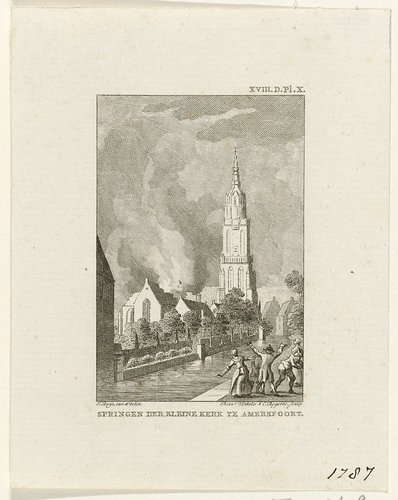
\includegraphics[width=\linewidth]{./Images/Chapter03/example_1.jpg}
\endminipage
\minipage{0.3\textwidth}
  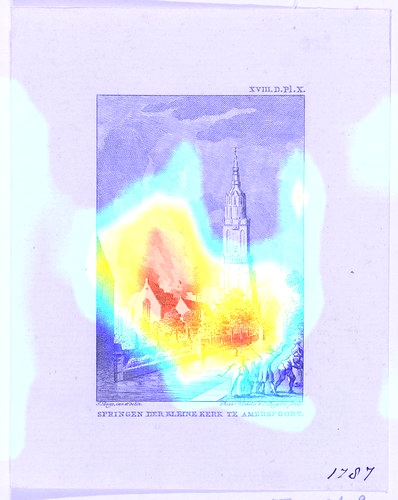
\includegraphics[width=\linewidth]{./Images/Chapter03/imagenet_saliencies_1.jpeg}
\endminipage
\minipage{0.3\textwidth}
  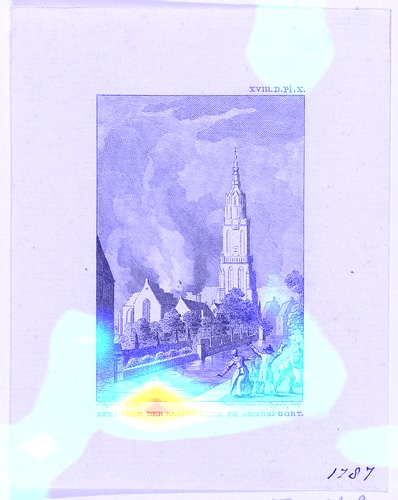
\includegraphics[width=\linewidth]{./Images/Chapter03/rijksnet_saliencies_1.jpeg}
\endminipage

\minipage{0.3\textwidth}
  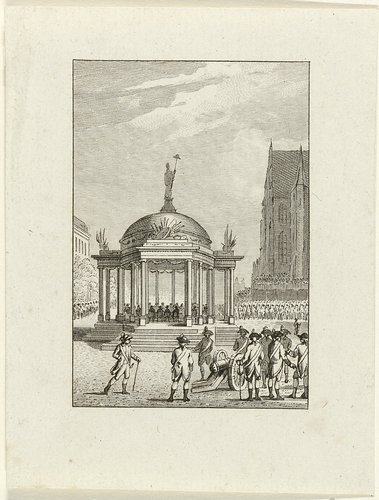
\includegraphics[width=\linewidth]{./Images/Chapter03/example_2.jpg}
\endminipage
\minipage{0.3\textwidth}
  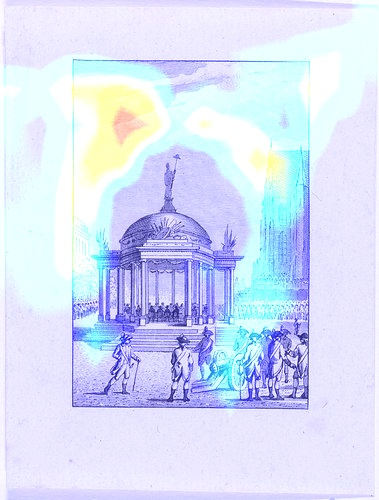
\includegraphics[width=\linewidth]{./Images/Chapter03/imagenet_saliencies_2.jpeg}
\endminipage
\minipage{0.3\textwidth}
  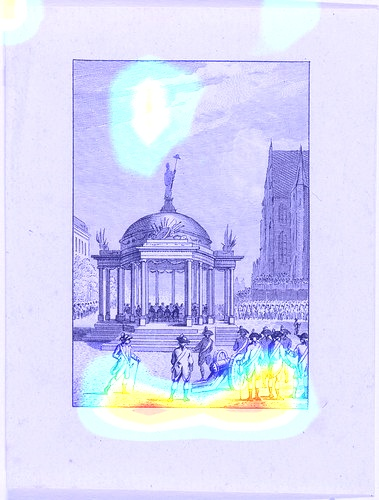
\includegraphics[width=\linewidth]{./Images/Chapter03/rijksnet_saliencies_2.jpeg}
\endminipage

\caption{Add caption}
\label{fig:saliency_maps}
\end{figure*}


These observations can be related to parallel insights in authorship attribution research \cite{stamatatos:2009}, an established task from Natural Language Processing that is highly similar in nature to artist recognition. In this field, preference is typically given to high-frequency function words (articles, prepositions, particles etc.) over content words (nouns, adjectives, verbs, etc.), because the former are generally considered to be less strongly related to the specific content or topic of a work. As such, function words or stop words lend themselves more easily to attribution across different topics and genres. In art history, strikingly similar views have been expressed by the well-known scholar Giovanni Morelli (1816-1891), who published seminal studies in the field of artist recognition \cite{wollheim:1972}. In Morelli's view too, the attribution of a painting could not happen on the basis of the specific content or composition of a painting, because these items were too strongly influenced by the topic of a painting or the wishes of a patron. Instead, Morelli proposed to base attributions to so-called \emph{Grundformen} or small, seemingly insignificant details that occur frequently in all paintings and typically show clear traces of an artist's individual style, such as ears, hands or feat, a painting's function words, so to speak. The saliency maps above reveal a similar shift in attention when the ImageNet weights are adapted on the Rijksmuseum data: instead of focusing on higher-level content features, the network shifts its attention to lower layers in the network, seemingly focusing on insignificant details, that nevertheless appear crucial to perform artist attribution.


\section{Conclusion} 
\label{sec:conclusion}
 
This paper provides insights about the potential that the field of TL has for art classification. We have investigated the behavior of DCNNs which have been originally pre-trained on a very different classification task and shown how their performances can be improved when these networks are fine tuned. Moreover, we have observed how such neural architectures perform better than if they are trained from scratch and develop new saliency maps that can provide insights about what makes these DCNNs outperform the ones that are pre-trained on the ImageNet dataset. Such saliency maps reflect themselves in the development of new features, which can then be successfully used by the DCNNs when classifying heritage objects that come from different heritage collections. It turns out that the fine tuned models are a better alternative to the same kind of architectures which are pre-trained on ImageNet only, and can serve the CV community which will deal with similar machine learning problems.

As future work, we aim to investigate whether the results that we have obtained on the Antwerp dataset will also apply to a larger set of smaller heritage collections. Furthermore, we want to explore the performances of densely connected layers \cite{huang2017densely} and understand which layers of the currently analyzed networks contribute the most to their final classification performances. This might allow us to combine the best parts of each neural architecture into one single novel DCNN which will be able to tackle all three classification tasks at the same time. 


 % Transfer Learning

\cleardoublepage % Empty page before the start of the next part


\part{Transfer Learning for Deep Supervised Learning} % First part of the thesis

% Chapter X

\chapter{Chapter Title} % Chapter title

\label{ch:name} % For referencing the chapter elsewhere, use \autoref{ch:name} 

%----------------------------------------------------------------------------------------

\section{Section Title}

Content

%------------------------------------------------

\subsection{Subsection Title}

Content

%------------------------------------------------

\subsection{Subsection Title}

Content

%----------------------------------------------------------------------------------------

\section{Section Title}

Content % ECCV paper
\chapter{Novel Datasets for Transfer Learning}
\label{ch:minerva}

\begin{remark}{Outline}

	In this chapter, we continue studying the transfer learning properties of convolutional neural networks trained on non-natural image distributions. To facilitate this process, we present MINERVA, a novel dataset that can be used both for object classification as for object detection. We report thorough experiments that highlight the challenges that can arise from using MINERVA as a computer vision testbed, while at the same time, we further characterize the benefits that can come from adopting transfer learning training strategies. The structure of this chapter is the following: in Sec. \ref{sec:cv_challenges} we describe some of the limitations that currently define the field of computer vision and that have served as inspiration for the development of our newly introduced dataset. In Sec. \ref{sec:minerva_dataset} we present MINERVA, we thoroughly explain how its images have been collected and annotated, and how the resulting splits have served for the experiments that are presented in Sec. \ref{sec:benchmarking}. We then report and discuss the results of our experiments in Sec. \ref{sec:minerva_results} and Sec. \ref{sec:discussion} respectively, before ending the chapter by identifying possible avenues for future work in Sec. \ref{sec:future_work}. 

\vspace{5mm}
\textit{This chapter is an extended version of the publication \citet{sabatelli2021advances}.}
\label{ch:minerva_paper}


\end{remark}


\section{Challenges of Modern Computer Vision}
\label{sec:cv_challenges}

If it is true that the results presented in the previous chapter show that it is possible to transfer pre-trained convolutional neural networks to non-natural image datasets successfully, it is equally true that some limitations might still need to be addressed. Above all, the need to fine-tune the networks instead of simply using them as feature extractors. As demonstrated by the experiments performed on the third classification problem of the Rijksmuseum dataset, it is clear that pre-trained models might only learn features that are relevant for their respective source task $\mathcal{T}_S$ (ImageNet), which therefore might result in unsatisfying performance when an off-the-shelf training strategy is used. While this is a result that does not come as a surprise, as it would be unreasonable to expect pre-trained networks to act as universal feature extractors, this limitation can still have some important practical implications since it can prevent the deployment of computer vision systems outside the domain of natural images. As a  practical example, let us consider the first image presented in Fig. \ref{fig:fails} and the computer vision task of object detection. We tackle this task with an object detector that is pre-trained on natural images only and that, therefore, has never seen any images coming from a domain other than the source domain $\mathcal{D}_S$. From the model's performance, it is clear that only one out of the two predictions made by the network is appropriate, as it fails in detecting the musical instrument depicted in the image by wrongly classifying it as a ``frisbee''. While certainly reasonable and fully justifiable, this kind of performance is the result of some limitations that currently characterize modern Computer Vision (CV), which we summarize as follows:

\begin{itemize}
	\item \textcolor{RoyalBlue}{Photorealism and Data Scarcity:} it is well known that modern CV strongly gravitates towards photorealistic material since most of the datasets that are used in the field are representative of digitized, or born-digital, versions of photographs. Nevertheless, datasets like MNIST, CIFAR-10/100 and the already mentioned ImageNet play a crucial role in today's rapid development of the field, as they are constantly used as benchmarks by the community. While certainly suitable for defining different challenging CV tasks, it is worth noting that these datasets are also only partially representative of the physical world, as they do not actively attempt to distort the reality they depict. Unfortunately, datasets going beyond the photorealistic domain are either much rarer, or are not as popular as their photorealistic counterparts, a limitation that results into pre-trained models that fail in performing well when used outside from the natural world (see again first image of Fig. \ref{fig:fails}).  

	\item \textcolor{RoyalBlue}{Modern Training Classes:} the performance depicted in the first image of Fig. \ref{fig:fails} can largely be attributed to the fact that the model used for detecting the objects in the image has never been explicitly trained on images of musical instruments. As a result its predictions can only tend to be representative of the classes that have governed the training process. While this behavior has only to be expected, it can still serve as a surrogate for highlighting an important limitation of modern object detection datasets: datasets are not as diversified and heterogeneous as one might expect. As an example let us consider the popular Pascal-Voc \cite{everingham2010pascal} and MS-COCO \cite{lin2014microsoft} datasets. The first one tackles the detection of 20 classes, out of which more than a third constitute different kinds of transportation systems, such as ``trains'', ``boats'', ``motorcycles'' and ``cars''. The latter, albeit more complex, mostly represents objects that are representative of the highly technological world we currently live in, with classes such as ``microwave'', ``laptop'' and ``remote control''. In practice, this results in models that gravitate towards detecting objects in an image that are modern, a behavior that hurts not-technological classes such as the ``person'' one, which should, but unfortunately is not, be detected in the second image of Fig. \ref{fig:fails}.     

	\item \textcolor{RoyalBlue}{Model Robustness:} the aforementioned limitation also results into models that learn features that are hardly general enough for successfully tackling different representations of the same class. As an example, let us consider the last image of Fig. \ref{fig:fails}: we can see that a model pre-trained on MS-COCO successfully detects the persons represented in the paintings only as long as their pose corresponds to a pose that can easily be found in the images depicting persons in photorealistic datasets. As soon as a person is depicted in a pose different from the one that usually characterizes a person in a photorealistic dataset (sitting or standing), then a pre-trained network mistakenly detects it as an animal.   
\end{itemize}

\begin{figure}[ht!]
\centering
  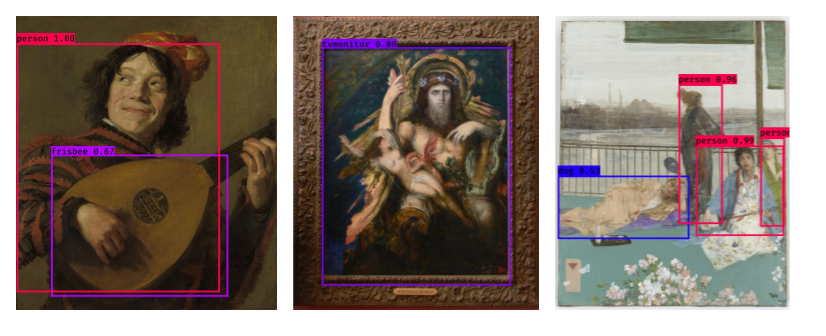
\includegraphics[width=\linewidth]{./Images/Chapter05/fails}
  \caption{Some examples that show the limitations of object detectors that are trained on photorealistic images only. In the first image, we see how a model confidently detects a ``frisbee'' for a ``lute'', while in the second image, we can observe how next to being unable to detect the people in the painting, it also mistakenly detects the frame as a ``tv-monitor''. Similar limitations can be observed in the third image, where we can see that the persons within the painting are only correctly detected as long as they are either sitting or standing.}
  \label{fig:fails}
\end{figure}

This chapter takes inspiration from these limitations and uses them as a surrogate for introducing novel datasets that can be used as a benchmark for CV researchers. The purpose of such datasets is twofold: on the one hand, they represent, at least in part, a solution to the aforementioned issues that currently characterize CV, while on the other hand, they allow us to continue studying the transfer learning properties of convolutional neural networks which we started exploring in the previous chapter.  

\section{The MINERVA Dataset}
\label{sec:minerva_dataset}

We now introduce MINERVA, a novel annotated dataset that can be used for object detection. More specifically, the main task that we present is that of the detection of musical instruments in non-photorealistic, unrestricted image collections from the artistic domain. We start by describing how its images have been first collected and then annotated, while we then move on towards quantitatively characterizing the dataset from a machine learning perspective.    

\subsection{Data Collection}
The images constituting MINERVA come from three different data sources, which allow the dataset to be highly varied and unrestricted. Its images cover a large range of periods, genres, and materials and are both of photorealistic and not-photorealistic nature as visually represented in Fig. \ref{fig:minerva_dataset}. The three data sources are the following:
\begin{itemize}
	\item RIDIM: which stays for \textit{Repertoire International d'Iconographie Musicale} is an international digital inventory for musical iconography that functions as a reference image database. Developed and curated by \citet{green2013ridim} it has been designed to facilitate the discovery of music-related artworks. Among the three different considered data sources, the images coming from the RIDIM collection are the ones of the highest quality in terms of resolution.
	\item RMFAB/RMAH: which stays for \textit{Royal Museums of Fine Arts of Belgium} and \textit{Royal Museums of Art and History}. These images come from a larger pool of digitized images that have been manually selected based on whether they included depictions of musical instruments or not. Among the different data sources, the amount of images coming from RMFAB/RMAH within MINERVA is the lowest compared to the other two data sources. These images are of midrange resolution.
	\item Flickr: is a well-known image hosting service from which we downloaded a large dataset of images depicting musical instruments in the visual arts pre-dating 1800. Most of the images present within MINERVA come from Flickr, although their resolution is not always on par with the one of the previous two data sources.  
\end{itemize}

Once all these images have been collected we have started the labeling process.


\begin{figure}[ht!]
\centering
  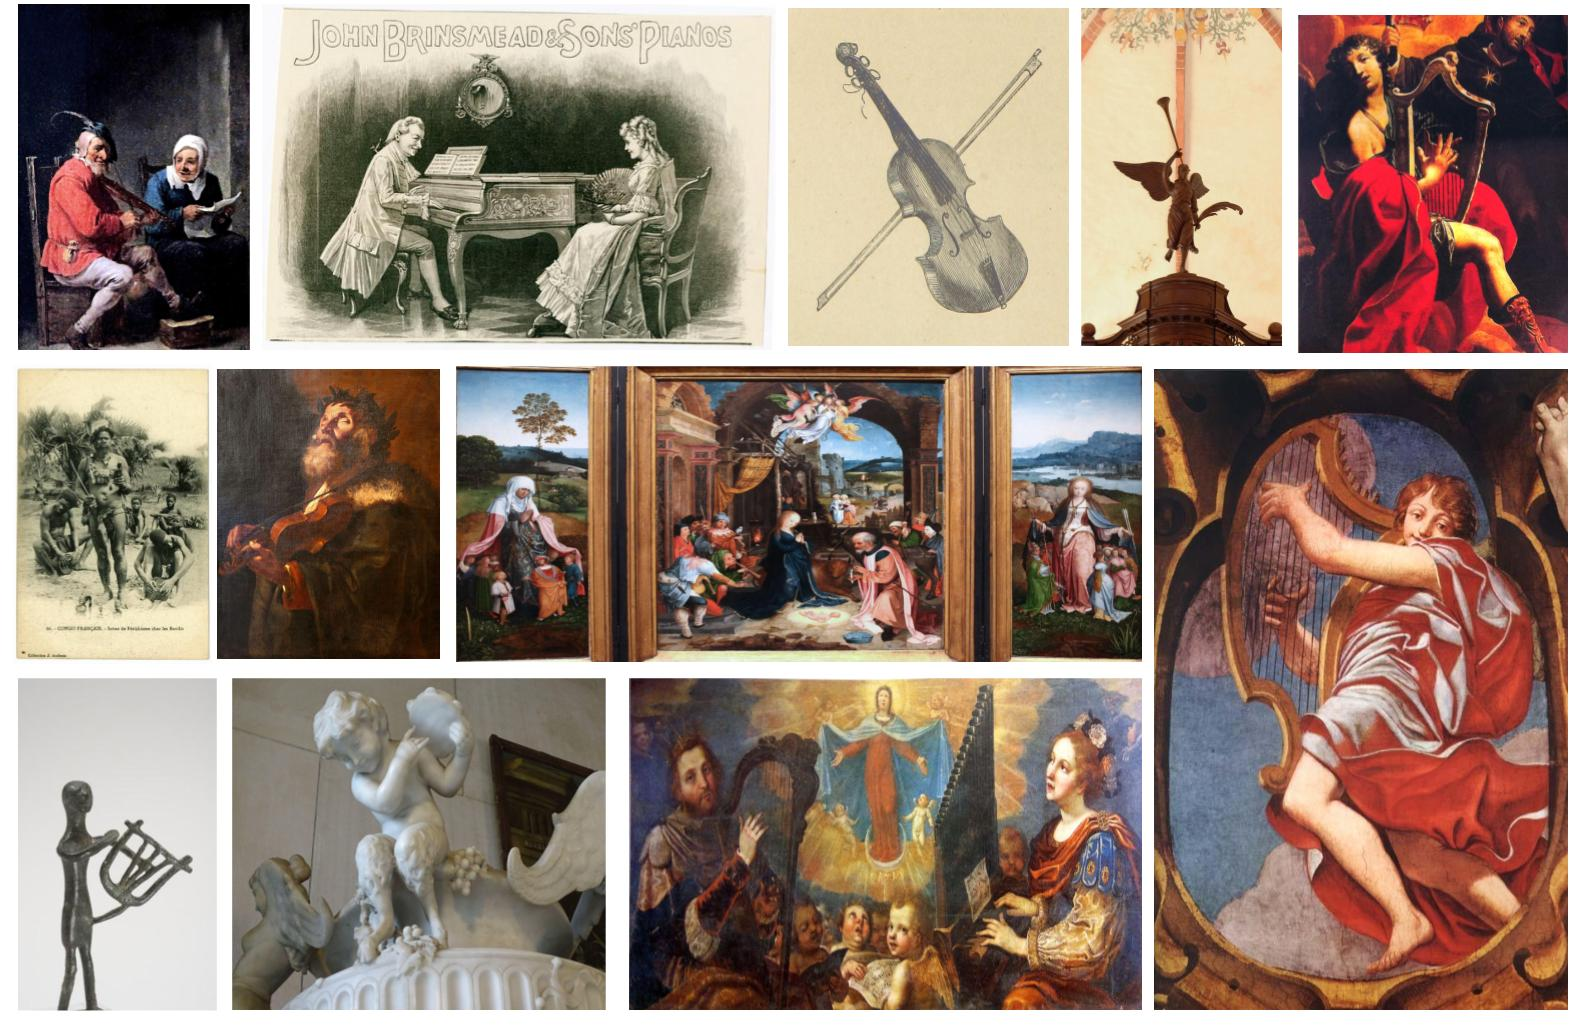
\includegraphics[width=\linewidth]{./Images/Chapter05/minerva}
  \caption{Samples from Minerva.}
  \label{fig:minerva_dataset}
\end{figure}

\subsection{Annotation Process}

We manually annotated almost $10000$ instruments by using the conventional method of rectangular bounding boxes. To this end, we have used the open-source \texttt{Cytomine} software \cite{maree2016collaborative}, a rich web environment that allows highly collaborative analysis of multi-gigapixel imaging data. Initially developed for facilitating the task of image annotation in biomedical informatics, \texttt{Cytomine} has already been widely used for the annotation and creation of several datasets \cite{mormont2018comparison}. However, it is worth noting that its use within the present study is among the very first ones which use the software outside the context of large-scale bioimaging data. All the individual instruments within MINERVA have been unambiguously identified and labeled by using their MIMO codes. The MIMO (Musical Instrument Museums Online) initiative is an international consortium, well known for its online database of musical instruments, aggregating data and metadata from multiple heritage institutions \cite{dolan2017mimo}. An important contribution of \citet{dolan2017mimo} is the development of a uniform metadata documentation standard for the field, including a multilingual vocabulary that can be used for identifying musical instruments in an interoperable manner. We have followed this metadata standard and manually labeled the previously collected images within \texttt{Cytomine} as visually represented in Fig. \ref{fig:cytomine_annotations}.

\begin{figure}[ht!]
\centering
  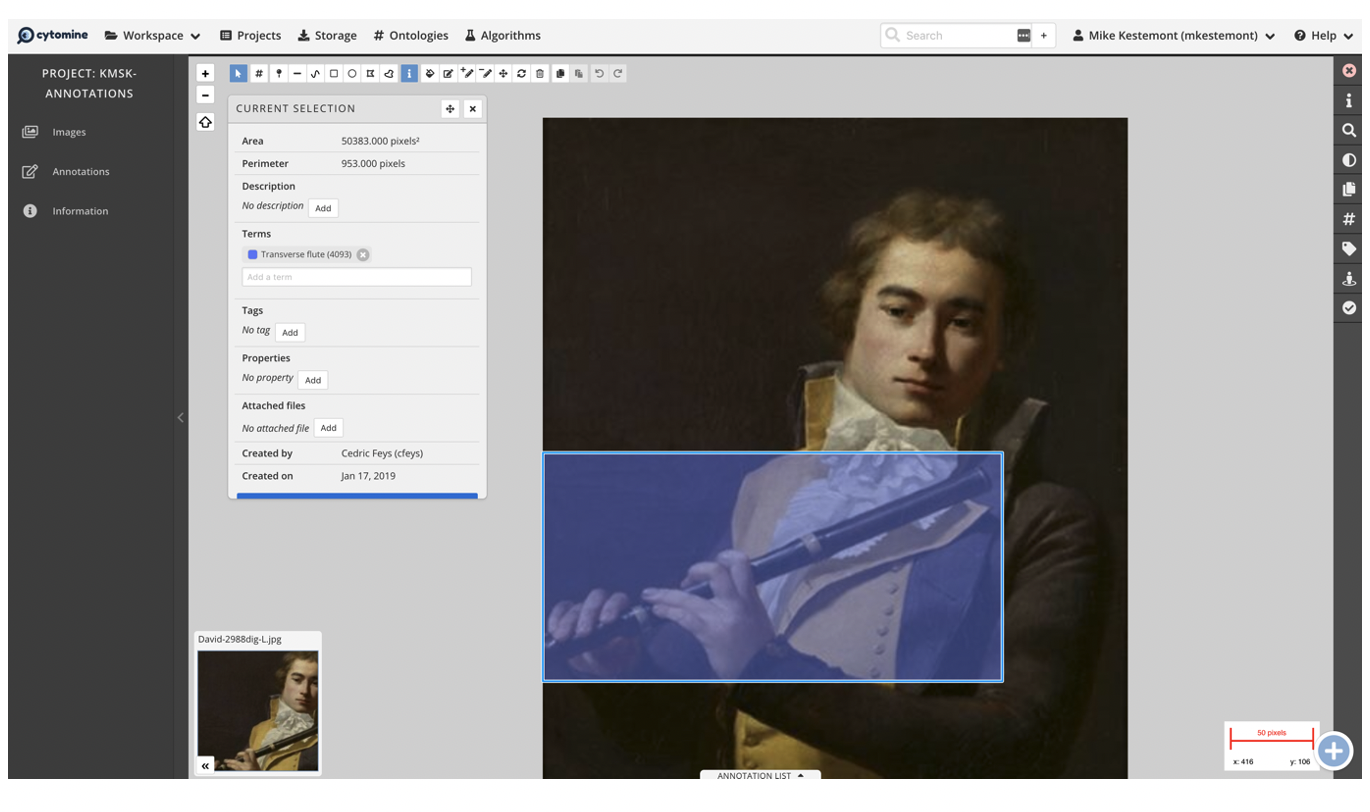
\includegraphics[width=\linewidth]{./Images/Chapter05/cytomine_annotations}
  \caption{A visualization of the annotation process performed with the \texttt{Cytomine} platform.}
  \label{fig:cytomine_annotations}
\end{figure}

\subsection{Versions and Splits}

MINERVA comes in four different, increasingly complex versions: \texttt{Minerva-0} which is arguably the easiest version of the dataset where the target task $\mathcal{T}_T$ simply consists in detecting whether a musical instrument is present within an image or not. We, therefore, do not yet consider the task of predicting the class of the detected instrument. The second version of the dataset is \texttt{Minerva-Hypernym} where the goal is that of detecting all the images present within \texttt{Minerva-0} and classify them according to their hypernym categories. All instruments present within MINERVA correspond to $5$ different hypernyms which define them as: ``stringed instruments'', ``wind instruments'', ``percussion instruments'', ``keyboard instruments'' and ``electronic instruments'. The last two versions of MINERVA are \texttt{Minerva-5} and \texttt{Minerva-10} where the goal is to detect and classify the instruments depicted in the images according to the top 5 or top 10 most occurring classes. These classes are: ``Lute'', ``Harp'', ``Violin'', ``Trumpet'', ``Shawn'', ``Bagpipe'', ``Organ'', ``Horn'', ``Rebec'' and ``Lyre''. Naturally, in \texttt{Minerva-5} we only consider the first $5$ of such classes, whereas in \texttt{Minerva-10} we consider all $10$ of them. Each version of the dataset comes with its training, validation, and testing splits, where we offer the guarantee that at least one of the instrument classes in the task is represented in each of the splits. Additionally, the splits are stratified so that the class distribution is approximately the same in each split. The number of images per split in each version is summarized in Table \ref{table:minerva_splits} where $N_t$ corresponds to the number of images present within the split, whereas $I_t$ denotes the number of total instruments. The hypernym version of the dataset is not reported as it shares the same images and splits as \texttt{Minerva-0} (they both contain all instruments). However, a distribution of the hypernym classes within \texttt{Minerva-Hypernym} is reported in Fig. \ref{fig:hypernym_distribution}. All splits have been created with the \texttt{scikit-learn} software \cite{pedregosa2011scikit} by using $50\%$ of the images for training and the remaining $50\%$ for validation and testing ($25\%$ respectively). 

\begin{table}[ht!]
\caption{An overview reporting how many images $N_t$ and instruments $I_t$ are present within the splits of the \texttt{Minerva-0, Minerva-5} and \texttt{Minerva-10} versions of the MINERVA dataset.}
	\begin{tabular}{l|rr|rr|rr} \hline
	$\mathcal{T}_T$ &  \multicolumn{2}{c}{training-set} & \multicolumn{2}{|c|}{validation-set} & \multicolumn{2}{c}{testing-set}\\
& $N_t$ & $I_t$ & $N_t$ & $I_t$ & $N_t$ & $I_t$ \\\hline \hline
\texttt{Minerva-0} & 1857 & 4243 & 1137 & 2288 & 1182 & 2102 \\
\texttt{Minerva-5} & 952 & 1589 & 540 & 852 & 721 & 1173\\
\texttt{Minerva-10} & 1227 & 2147  & 680 & 1127 & 897 & 1506 \\
\hline

\end{tabular}

\label{table:minerva_splits}
\end{table}

\begin{figure}[htb!]
	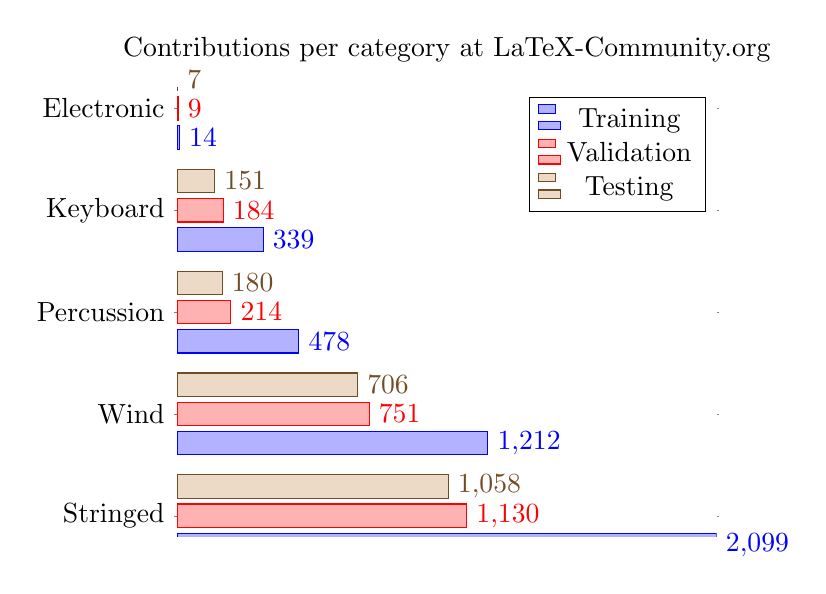
\begin{tikzpicture}
  \begin{axis}[title  = Contributions per category
                          at LaTeX-Community.org,
    xbar,
    bar width=.3cm,
    y axis line style = { opacity = 0 },
    axis x line       = none,
    tickwidth         = 1pt,
    enlarge y limits  = 0.05,
    enlarge x limits  = 0.001,
    symbolic y coords = {Stringed, Wind, Percussion,Keyboard, Electronic},
    nodes near coords,
  ]
\addplot coordinates {(2099,Stringed) (1212,Wind) (478,Percussion) (339,Keyboard) (14,Electronic)};
\addplot coordinates {(1130,Stringed) (751,Wind) (214,Percussion) (184,Keyboard) (9,Electronic)};
\addplot coordinates {(1058,Stringed) (706,Wind) (180,Percussion) (151,Keyboard) (7,Electronic)};
\legend{Training,Validation,Testing}

\end{axis}
\end{tikzpicture}

\iffalse
\end{axis}
\end{tikzpicture}
\fi

	\caption{A visual representation of the distribution of the hypernym classes that are present within \texttt{Minerva-0} and that define the \texttt{Minerva-Hypernym} benchmark.}
	\label{fig:hypernym_distribution}
\end{figure}


\section{Benchmarking}
\label{sec:benchmarking}

While MINERVA has been created with the primary intention of serving as a novel dataset for object detection, it can nevertheless still be used to test the classification performance of convolutional neural networks. Although it could be argued that this task could be easier than object detection, it is still of high interest as it provides a novel benchmark for further characterizing the transfer learning properties of neural networks that we started studying in the previous chapter. Therefore, we hereafter report results both for \textcolor{RoyalBlue}{classification} experiments as well as for \textcolor{RoyalBlue}{object detection} experiments. In the first section, we consider the target task $\mathcal{T}_T$ of classifying the bounding boxes that have been annotated in MINERVA as standalone images, while in the second section, we aim at both detecting and classifying the content of the potentially detected bounding boxes. We hereafter describe the experimental protocol used for both sets of experiments in detail.

\subsection{Classification}
The experimental setup used for the classification experiments largely builds on top of the study that we presented in Chapter \ref{ch:tl_natural_to_non_natural}. We continue to explore whether popular neural architectures, which have obtained state-of-the-art results on the ImageNet benchmark, can perform equally well when trained on datasets of non-natural images. To this end, we again consider the well known VGG19 \cite{simonyan2014very}, InceptionV3 \cite{szegedy2016rethinking} and ResNet50 \cite{xie2017aggregated} neural architectures. As done in the previous chapter, we keep investigating the effect that different weight initialization strategies have on the final performance of the networks to characterize further the potential benefits that can come from adopting transfer learning. Specifically, we train the three considered neural architectures by following three different initialization strategies: ``random'' which simply initializes the model's parameters after following He's weight initialization strategy \cite{he2015delving}, ``ImageNet'' which instead uses the weights that are obtained after training the networks on the ImageNet source task $\mathcal{T}_S$, and ``RijksNet'' which are models that are trained both on the ImageNet dataset and on the Rijksmuseum collection, and that were also used for the final experiments reported in the previous chapter. As the benefits of fully fine-tuning the models over using them as off-the-shelf feature extractors were clear from the results obtained in Chapter \ref{ch:tl_natural_to_non_natural}, we now limit our analysis to this transfer-learning approach solely. We train all networks with the Adam optimizer \cite{kingma2014adam} and by using an initial learning rate of $0.001$. As already done for the previous study, we again controlled the training process by using early stopping and by interrupting the training regime as soon as the validation loss did not decrease for five epochs in a row. Naturally, all networks minimize the categorical cross-entropy loss function.

\subsection{Object Detection}
\label{sec:object_detection_exp}

For this set of experiments we explore the performance of a YOLO object detector \cite{redmon2017yolo9000}, a popular neural architecture that has obtained state-of-the-art results on the MS-COCO object detection benchmark. YOLO treats the task of object detection as a standard regression problem by dividing an image into a $S\times S$ grid and by predicting for each grid cell $B$ bounding boxes and $C$ class probabilities. The main assumption behind YOLO is that any of the $S\times S$ cells contains at most the center of one single object, therefore for every image, cell index $i=1,...,S\times S$, predicted box $j=1,...,B$ and class index $c=1,...,C$ we have the following components: 

\begin{itemize}
	\item $\mathbb{1}_{i}^\text{obj}$ which is $1$ if there is an object in cell $i$, and $0$ otherwise;
	\item $\mathbb{1}_{i,j}^\text{obj}$ which is $1$ if there is an object in cell $i$ and predicted box $j$ that is the most fitting one, whereas is $0$ otherwise; 
	\item $p_{i,c}$ which is $1$ if there in an object of class $c$ in cell $i$, and 0 otherwise;
	\item $x_i,y_i,w_i,h_i$ which are the coordinates of an annotated bounding box that are defined only if $\mathbb{1}_{i}^{\text{obj}}=1$;
	\item $c_{i,j}$ which is the IoU between the predicted box and the ground truth target.
\end{itemize}

At training, YOLO computes the value of the $\mathbb{1}_{i,j}^{\text{obj}}$ for each image together with the respective $c_{i,j}$, and then minimizes the following multi-part loss function:

\begin{equation}
\begin{split}
& \lambda_\text{coord} \sum_{i=1}^{S \times S} \sum_{j=1}^B \mathbb{1}_{i,j}^\text{obj} \left( (x_i - \hat{x}_{i,j})^2 + (y_i - \hat{y}_{i,j})^2 + (\sqrt{w_i} - \sqrt{\hat{w}_{i,j}})^2 + (\sqrt{h_i} - \sqrt{\hat{h}_{i,j}})^2\right)\\\\
& + \lambda_\text{obj} \sum_{i=1}^{S \times S} \sum_{j=1}^B \mathbb{1}_{i,j}^\text{obj} (c_{i,j} - \hat{c}_{i,j})^2 + \lambda_\text{noobj} \sum_{i=1}^{S \times S} \sum_{j=1}^B (1-\mathbb{1}_{i,j}^\text{obj}) \hat{c}_{i,j}^2  \\\\
& + \lambda_\text{classes} \sum_{i=1}^{S \times S} \mathbb{1}_i^\text{obj} \sum_{c=1}^C (p_{i,c} - \hat{p}_{i,c})^2
\end{split} 
\end{equation}

\noindent where $\hat{p}{i,c}$, $\hat{x}{i,j}$, $\hat{y}{i,j}$, $\hat{w}{i,j}$, $\hat{h}{i,j}$ and $\hat{c}{i,j}$ are the predictions of the network.

In our experiments, we use the YOLO-V3 version of the network introduced by \citet{redmon2018yolov3} and initialize it with the weights that are obtained after training the network on the MS-COCO dataset. Regarding the stochastic optimization procedure, we use two different optimizers: we train the network with the Adam optimizer for the first 10 epochs, while we then use the RMSprop optimizer for the remaining training epochs, which are again controlled through early stopping. To assess the final performance of the model, we follow an evaluation protocol that is typical for object detection problems in CV \cite{lin2014microsoft}. Each detected bounding box is compared to the bounding box, which has been annotated on the \texttt{Cytomine} platform. We only consider bounding boxes for which the confidence level is $\geq 0.05$, following the protocol established by \citet{everingham2010pascal}. We then compute the ``Intersection over Union'' (IoU) for measuring how much the detected bounding boxes differ from the ground-truth ones. To assess whether a prediction can be considered as a true positive or a false positive, we define two increasingly restrictive metrics: first, IoU $\geq10$ and, secondly, IoU $\geq50$. This approach is inspired by the work of \citet{gonthier2018weakly}, where the authors report results for both IoU thresholds when assessing the performance of their weakly supervised learning system on the IconArt dataset.

\section{Results}
\label{sec:minerva_results}

\subsection{Quantitative Analysis}
\label{sec:quantitative_analysis}
\paragraph{\textbf{\uppercase{C}lassification}}

We start by discussing the results obtained with our classification experiments. The performance of all models is reported in Tables \ref{table:minerva_no_tl_results}, \ref{table:minerva_tl_results} and \ref{table:minerva_rijks_results}, where we present the accuracy that the networks have obtained on the different MINERVA testing sets, together with their respective F1 scores. To this end for a given class $c$, a ground truth label $y$ and a model's prediction $\hat{y}$, let us introduce the notions of precision and recall. The first is computed as:
\begin{equation}
	\text{P}(c)=p(y=c|\hat{y}=c)=\frac{TP}{TP+FP},
\end{equation}
while the latter as
\begin{equation}
	\text{R}(c)=p(\hat{y}=c|y=c)=\frac{TP}{TP+FN}.
\end{equation}
Both quantities can be used for computing the F-1 score as follows:
\begin{equation}
	\text{F1}(c)=2 \cdot \frac{\text{P}(c)\cdot\text{R}(c)}{\text{P}(c)+\text{R}(c)}.
\end{equation}
Similarly to the results reported in Chapter \ref{ch:tl_natural_to_non_natural} we again report the best performing architecture in a green cell, while the second-best performing model in a yellow one.  

We can start by observing that among all the results presented in the three different tables, the best performing models are either the ones reported in Table \ref{table:minerva_tl_results} or the ones presented in Table \ref{table:minerva_rijks_results}. This confirms the results that were presented in the previous chapter: fine-tuning pre-trained models yields significantly better results than training models from scratch, even when the source and the target tasks can be particularly different (as is the case for musical instruments classification). While the results of this study confirm the conclusions that were drawn at the end of Chapter \ref{ch:tl_natural_to_non_natural}, they also provide some additional insights that were not observed before. First, it appears that the best performing architecture is not ResNet50 anymore, but rather the arguably older InceptionV3, a result which seems to suggest that there is no overall best-performing architecture for all target tasks $\mathcal{T}_T$, and that the best architecture is highly problem dependent. Second, and perhaps arguably more surprising, we can also see that differently from what was observed in the last experiment in Chapter \ref{ch:tl_natural_to_non_natural}, it appears to be more beneficial to transfer models pre-trained on ImageNet only, instead of models that are additionally trained on the Rijksmuseum collection. Indeed, as can be observed by the results presented in Tables \ref{table:minerva_tl_results} and \ref{table:minerva_rijks_results}, the latter pre-training strategy outperforms the first one only when the ResNet50 and the InceptionV3 architectures are trained on the \texttt{Minerva-5} benchmark. These results can be explained as follows: in Chapter \ref{ch:tl_natural_to_non_natural} the target task $\mathcal{T}_T$ tackled with a model pre-trained on the Rijksmuseum collection corresponded to the original source task $\mathcal{T}_S$ (classification of ``types'' and ``artists''). In these experiments, however, albeit coming from similar domains, the considered source task $\mathcal{T}_S$ and target task $\mathcal{T}_T$ are unrelated, which could work in favor of an arguably more general ImageNet weight initialization.


\begin{table}[ht!]
	\caption{Results obtained when classifying the bounding boxes of the three different MINERVA benchmarks with models that do not come as pre-trained on any sort of source task $\mathcal{T}_S$. We can see that their performance is significantly worse than the one that is obtained when the same models come as pre-trained (see Table \ref{table:minerva_tl_results} and Table \ref{table:minerva_rijks_results}).}
\resizebox{\columnwidth}{!}{%
	\begin{tabular}{l|cc|cc|cc} \hline
	$\mathcal{T}_T$ &  \multicolumn{2}{c}{ResNet50} & \multicolumn{2}{|c|}{InceptionV3} & \multicolumn{2}{c}{VGG19}\\
			& Accuracy ($\%$) & F1 & Accuracy ($\%$) & F1 & Accuracy $(\%)$ & F1 \\\hline \hline
	\texttt{Minerva-Hypernym} & 50.33 & 13.39 & 51.80 & 14.02 & 50.12 & 13.12 \\
	\texttt{Minerva-5} & 40.83  & 21.88 & 40.49 & 21.65 & 41.26 & 22.01\\
	\texttt{Minerva-10} & 32.85 & 0.09  & 32.18 & 0.09 & 19.72 & 0.03 \\
\hline
\end{tabular}
%
}
\label{table:minerva_no_tl_results}
\end{table}



\begin{table}[ht!]
	\caption{Results obtained when classifying the bounding boxes of the three different MINERVA benchmarks after adapting transfer learning and considering the ImageNet dataset as the only source task $\mathcal{T}_S$. We observe that, compared to the results presented in Table \ref{table:minerva_no_tl_results}, this approach yields significant benefits, therefore confirming the results presented in Chapter \ref{ch:tl_natural_to_non_natural}.}
\resizebox{\columnwidth}{!}{%
	\begin{tabular}{l|cc|cc|cc} \hline
	$\mathcal{T}_T$ &  \multicolumn{2}{c}{ResNet50} & \multicolumn{2}{|c|}{InceptionV3} & \multicolumn{2}{c}{VGG19}\\
			& Accuracy ($\%$) & F1 & Accuracy ($\%$) & F1 & Accuracy $(\%)$ & F1 \\\hline \hline
	\texttt{Minerva-Hypernym} & \cellcolor{yellow!25}{76.64} & \cellcolor{yellow!25}{58.56} & \cellcolor{green!25}{79.40} & \cellcolor{green!25}{60.07} & 76.54 & 57.39 \\
	\texttt{Minerva-5} & 60.41  & 49.10 & 72.06 & 68.89 & 70.43 & 68.42\\
	\texttt{Minerva-10} & 55.37 & 41.65  & \cellcolor{green!25}{60.1} & \cellcolor{green!25}{45.12} & 44.22 & 40.12 \\
\hline
\end{tabular}
%
}
\label{table:minerva_tl_results}
\end{table}


\begin{table}[ht!]
	\caption{Results obtained when classifying the bounding boxes of the three different MINERVA benchmarks after adapting transfer learning and considering the ImageNet and the Rijksmuseum collection as source domains $\mathcal{D}_S$. Similarly to what was observed in Table \ref{table:minerva_tl_results}, we can again see that transfer learning yields significant benefits although this weight initialization strategy does mostly not outperform the more common ImageNet one.}
\resizebox{\columnwidth}{!}{%
	\begin{tabular}{l|cc|cc|cc} \hline
	$\mathcal{T}_T$ &  \multicolumn{2}{c}{ResNet50} & \multicolumn{2}{|c|}{InceptionV3} & \multicolumn{2}{c}{VGG19}\\
			& Accuracy ($\%$) & F1 & Accuracy ($\%$) & F1 & Accuracy $(\%)$ & F1 \\\hline \hline
	\texttt{Minerva-Hypernym} & 72.26 & 52.66 & \cellcolor{green!25}{75.80} & \cellcolor{green!25}{57.03} & 66.41 & 40.35 \\
	\texttt{Minerva-5} & 68.71  & 64.10 & \cellcolor{green!25}{73.66} & \cellcolor{green!25}{70.29} & 48.33 & 33.92\\
	\texttt{Minerva-10} & 52.85 & 41.55  & \cellcolor{green!25}{55.51} & \cellcolor{green!25}{44.77} & 37.52 & 15.22 \\
\hline
\end{tabular}
%
}
\label{table:minerva_rijks_results}
\end{table}


\paragraph{\textbf{\uppercase{O}bject \uppercase{D}etection}}
The results for this set of experiments are reported in terms of average precision as for each class; we report the area under the precision-recall curve that is obtained by setting IoU $\geq10$ and $\geq50$ as explained in Sec. \ref{sec:object_detection_exp}. We start by discussing the performance that is obtained after fine-tuning a pre-trained YOLO-V3 model on the \texttt{Minerva-0} benchmark, where, as a reminder, the goal is that of simply detecting a musical instrument within an image without classifying it. For an IoU $\geq 10$ we report an average precision of $35.33\%$, while for an IoU $\geq 50$, a final score of $22.31\%$. Both scores demonstrate that the model is successfully able to detect the musical instruments within MINERVA and that, on this task, its performance is on par with the one that is reported on more common object detection benchmarks \cite{lin2014microsoft}. More specifically, the model detects an instrument $1386$ times, out of which when an IoU $\geq 10$ is considered, $878$ detections correspond to true positives, whereas $508$ detections are false positives. Naturally, the model's performance decreases when an IoU $\geq 50$ is considered, as the amount of true positive detections decreases to $648$ and the number of false positives increases to $738$.

We report a similar quantitative analysis for the \texttt{Minerva-Hypernym}, \texttt{Minerva-5} and \texttt{Minerva-10} benchmarks. We do this in Tables \ref{table:minerva_detection_hypernyms}, \ref{table:minerva_5_detection} and \ref{table:minerva_10_detection} where we present the different average precision scores, and in Figures \ref{fig:detection_experiment_2}, \ref{fig:detection_experiment_3} and \ref{fig:detection_experiment_4}, where we visualize the true vs false positives detections. We can see that out of these three benchmarks, the \texttt{Minerva-Hypernym} one appears to be the most challenging one as it results in the worst-performing models independently from which IoU threshold is considered. We can observe from Fig. \ref{fig:detection_experiment_2} that the model can detect ``stringed instruments'' successfully, whereas its performance in detecting the remaining four hypernyms of the dataset is drastically worse. When it comes to the \texttt{Minerva-5} benchmark, we can observe from Table \ref{table:minerva_5_detection} that the model can successfully detect three instruments out of the five instruments which constitute this benchmark, namely ``Harps', ``Lutes'', and ``Violins''. These results are only second to the ones obtained on \texttt{Minerva-0}, although the considered target task $\mathcal{T}_T$ is now significantly harder. Similar detections have been obtained after fine-tuning the model on the \texttt{Minerva-10} benchmark. Here we can again observe (see Table \ref{table:minerva_10_detection} and Fig. \ref{fig:detection_experiment_4}) that the network can only successfully detect the first three most occurring instruments of the dataset, whereas for the ``Horn'', ``Bagpipe'' ``Rebec'' and ``Lyre'' classes no detections at all are made. 

\begin{table}[ht!]
	\caption{Average Precision ($\%$) obtained when fine-tuning a pre-trained YOLO-V3 object detector on the \texttt{Minerva-Hypernyms} dataset. We can observe that satisfying results are obtained for both IoU thresholds when it comes to the detection of stringed instruments, whereas detecting the remaining four hypernyms of MINERVA appears to be much more challenging.}
\resizebox{\columnwidth}{!}{%	
	\begin{tabular}{c|c|c|c|c|c||c}\hline
		& Stringed & Wind & Percussion & Keyboard & Electronic & Mean\\ \hline \hline 
	AP IoU $\geq10$ & 28.22         & 4.58      & 2.55           & 7.36  & 0   &  6.03  \\
	AP IoU $\geq50$ & 20.95         &  2.91    &  1.84          &  4.47       & 0 & 8.54 
\end{tabular}
%
}
\label{table:minerva_detection_hypernyms}
\end{table}


\begin{table}[ht!]
	\caption{Average Precision ($\%$) obtained on the \texttt{Minerva-5} benchmark. We can observe that the fine-tuned model successfully detects ``Harps'', ``Lutes'' and ``Violins'', whereas the detection of ``Shawns'' and ``Trumpets'' can be improved.}
\resizebox{\columnwidth}{!}{%	
	\begin{tabular}{c|c|c|c|c|c||c}\hline
		& Harp & Lute & Violin & Shawn & Trumpet & Mean\\ \hline \hline 
	AP IoU $\geq10$ & 55.60         & 36.51      & 12.21           & 1.75 & 1.3   &  21.47  \\
	AP IoU $\geq50$ & 46.80         &  26.93    &  7.64          &  1.01       & 1.07 & 16.69 
\end{tabular}
%
}
\label{table:minerva_5_detection}
\end{table}


\begin{table}[ht!]
	\caption{Average Precision ($\%$) obtained on the \texttt{Minerva-10} benchmark. Similarly to what was presented in Table \ref{table:minerva_5_detection}, we can again observe that the model successfully detects the first three most occurring instruments within the dataset, whereas it appears to perform poorly on the remaining instrument classes.}
\resizebox{\columnwidth}{!}{%	
	\begin{tabular}{c|c|c|c|c|c|c|c|c|c|c||c}\hline
		& Harp & Lute & Violin & Shawn & Trumpet  & Organ & Rebec & Lyre & Horn & Bagpipe & Mean\\ \hline \hline 
	AP IoU $\geq10$ &  46.88         &  33.74    &  6.73          &  0.59       & 1.83 & 6.1 & 0 & 0 & 0 & 0 & 9.58  \\
	AP IoU $\geq50$ & 39.81         &  25.40    &  4.82          &  0.59       & 0.14 & 6.1 & 0 & 0 & 0 & 0 & 7.68 
\end{tabular}
%
}
\label{table:minerva_10_detection}
\end{table}


\begin{figure}[htb!]
	\scalebox{0.8}{\begin{minipage}{.5\textwidth}
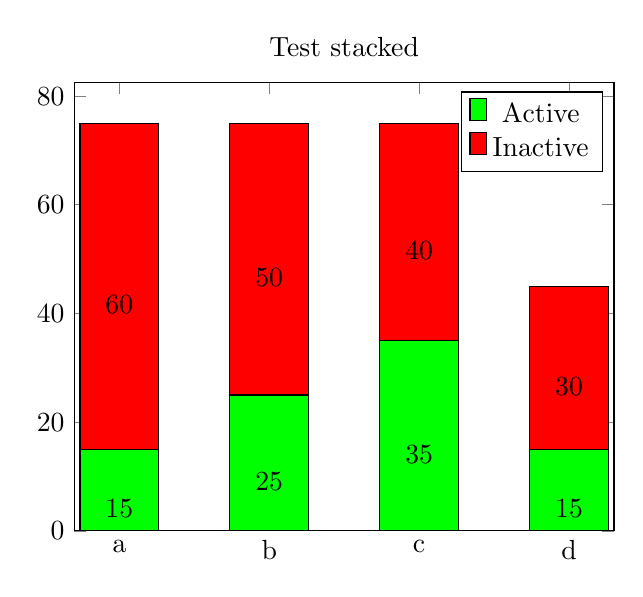
\begin{tikzpicture}
  \begin{axis}[
    title={Test stacked},
    ybar stacked, ymin=0,  
    bar width=10mm,
    symbolic x coords={a,b,c,d},
    xtick=data,
    nodes near coords, 
    nodes near coords align={anchor=north},%Move values in bar
    every node near coord/.style={
    },
  ]
  %Active
  \addplot [fill=green] coordinates {
({a},15)
({b},25)
({c},35)
({d},15)};
  %Inactive
  \addplot [fill=red] coordinates {
({a},60)
({b},50)
({c},40)
({d},30)};
  \legend{Active,Inactive}
  \end{axis}
 \end{tikzpicture}
 \end{minipage}
 \hspace{2.5cm}
\begin{minipage}{.5\textwidth}
 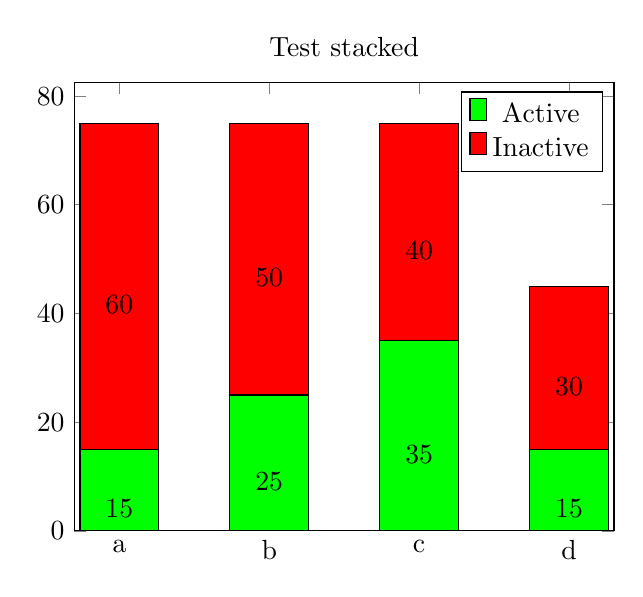
\begin{tikzpicture}
  \begin{axis}[
    title={Test stacked},
    ybar stacked, ymin=0,  
    bar width=10mm,
    symbolic x coords={a,b,c,d},
    xtick=data,
    nodes near coords, 
    nodes near coords align={anchor=north},%Move values in bar
    every node near coord/.style={
    },
  ]
  %Active
  \addplot [fill=green] coordinates {
({a},15)
({b},25)
({c},35)
({d},15)};
  %Inactive
  \addplot [fill=red] coordinates {
({a},60)
({b},50)
({c},40)
({d},30)};
  \legend{Active,Inactive}
  \end{axis}
 \end{tikzpicture}
 \end{minipage}

}
	\caption{True Positive (TP) vs False Positive (FP) analysis on the \texttt{Minerva-Hypernym} benchmark for IoU $\geq10$ and IoU $\geq50$.}
	\label{fig:detection_experiment_2}
\end{figure}



\begin{figure}[htb!]
	\scalebox{0.8}{\begin{minipage}{.5\textwidth}
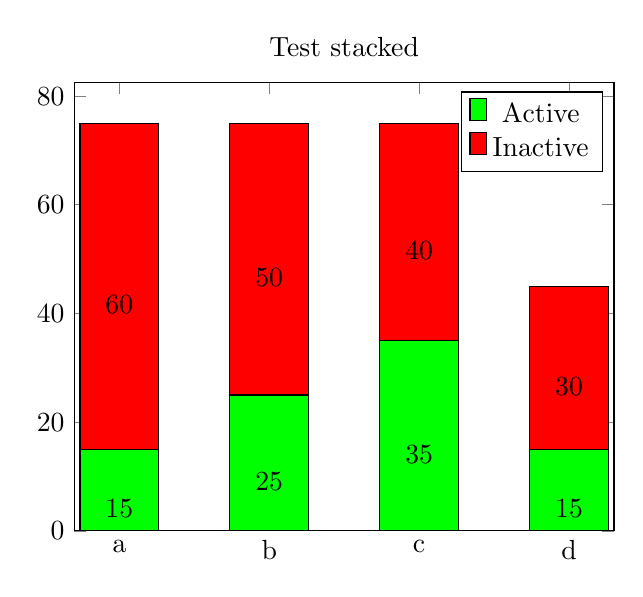
\begin{tikzpicture}
  \begin{axis}[
    title={Test stacked},
    ybar stacked, ymin=0,  
    bar width=10mm,
    symbolic x coords={a,b,c,d},
    xtick=data,
    nodes near coords, 
    nodes near coords align={anchor=north},%Move values in bar
    every node near coord/.style={
    },
  ]
  %Active
  \addplot [fill=green] coordinates {
({a},15)
({b},25)
({c},35)
({d},15)};
  %Inactive
  \addplot [fill=red] coordinates {
({a},60)
({b},50)
({c},40)
({d},30)};
  \legend{Active,Inactive}
  \end{axis}
 \end{tikzpicture}
 \end{minipage}
 \hspace{2.5cm}
\begin{minipage}{.5\textwidth}
 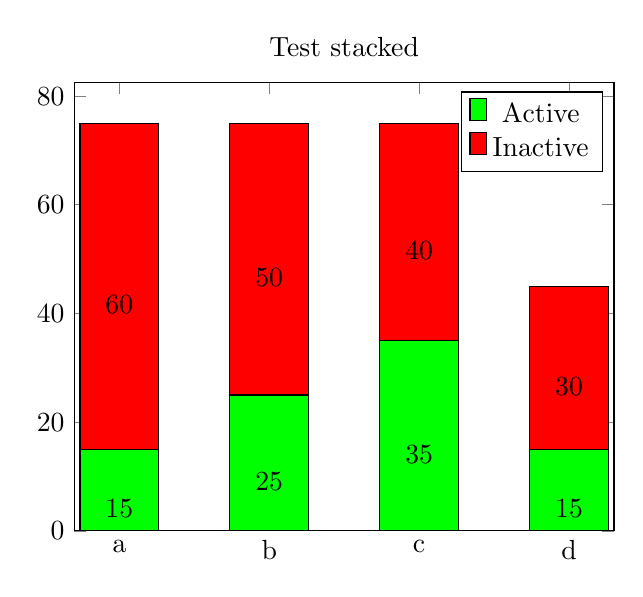
\begin{tikzpicture}
  \begin{axis}[
    title={Test stacked},
    ybar stacked, ymin=0,  
    bar width=10mm,
    symbolic x coords={a,b,c,d},
    xtick=data,
    nodes near coords, 
    nodes near coords align={anchor=north},%Move values in bar
    every node near coord/.style={
    },
  ]
  %Active
  \addplot [fill=green] coordinates {
({a},15)
({b},25)
({c},35)
({d},15)};
  %Inactive
  \addplot [fill=red] coordinates {
({a},60)
({b},50)
({c},40)
({d},30)};
  \legend{Active,Inactive}
  \end{axis}
 \end{tikzpicture}
 \end{minipage}

}
	\caption{True Positive (TP) vs False Positive (FP) analysis on the \texttt{Minerva-5} benchmark for IoU $\geq10$ and IoU $\geq50$.}
	\label{fig:detection_experiment_3}
\end{figure}


\begin{figure}[htb!]
	\scalebox{0.8}{\begin{minipage}{.5\textwidth}
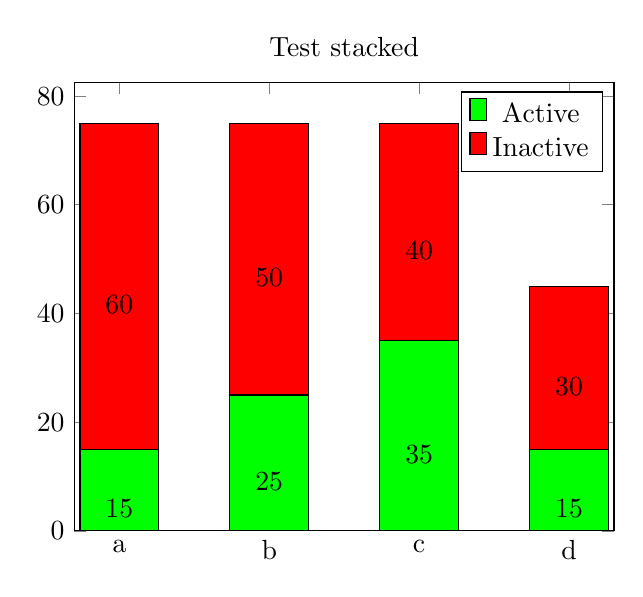
\begin{tikzpicture}
  \begin{axis}[
    title={Test stacked},
    ybar stacked, ymin=0,  
    bar width=10mm,
    symbolic x coords={a,b,c,d},
    xtick=data,
    nodes near coords, 
    nodes near coords align={anchor=north},%Move values in bar
    every node near coord/.style={
    },
  ]
  %Active
  \addplot [fill=green] coordinates {
({a},15)
({b},25)
({c},35)
({d},15)};
  %Inactive
  \addplot [fill=red] coordinates {
({a},60)
({b},50)
({c},40)
({d},30)};
  \legend{Active,Inactive}
  \end{axis}
 \end{tikzpicture}
 \end{minipage}
 \hspace{2.5cm}
\begin{minipage}{.5\textwidth}
 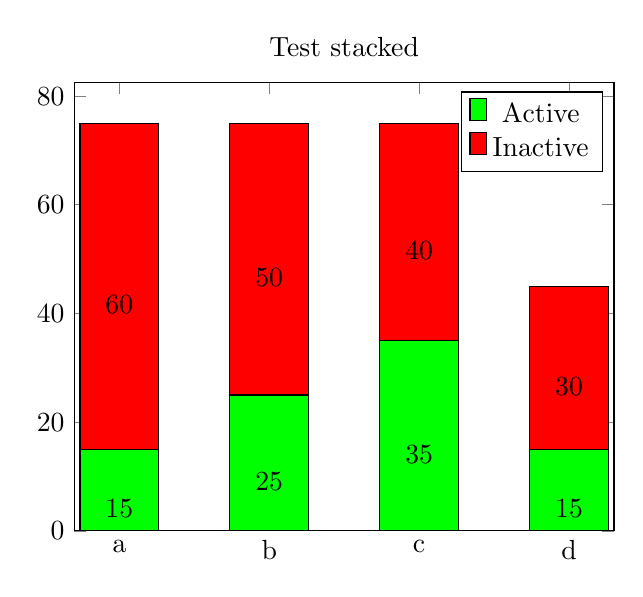
\begin{tikzpicture}
  \begin{axis}[
    title={Test stacked},
    ybar stacked, ymin=0,  
    bar width=10mm,
    symbolic x coords={a,b,c,d},
    xtick=data,
    nodes near coords, 
    nodes near coords align={anchor=north},%Move values in bar
    every node near coord/.style={
    },
  ]
  %Active
  \addplot [fill=green] coordinates {
({a},15)
({b},25)
({c},35)
({d},15)};
  %Inactive
  \addplot [fill=red] coordinates {
({a},60)
({b},50)
({c},40)
({d},30)};
  \legend{Active,Inactive}
  \end{axis}
 \end{tikzpicture}
 \end{minipage}

}
	\caption{True Positive (TP) vs False Positive (FP) analysis on the \texttt{Minerva-Hypernym} benchmark for IoU $\geq10$ and IoU $\geq50$.}
	\label{fig:detection_experiment_4}
\end{figure}



\subsection{Qualitative Analysis}
\label{sec:qualitative_analysis}
We now characterize the performance of the aforementioned fine-tuned models from a qualitative perspective. 

\paragraph{\textbf{\uppercase{O}bject \uppercase{C}lassification}}
For the classification experiments, we keep building on top of the study presented in the previous chapter and perform a qualitative evaluation of the models that is based on the visualization of saliency maps, as this allows us to investigate which visual properties in the image are exploited by the networks for correctly classifying the instruments in MINERVA. We hereafter report saliency maps that are obtained after fine-tuning an ImageNet pre-trained ResNet50 model on the \texttt{Minerva-Hypernym} benchmark, and that are computed with two different, gradient-based techniques: Grad-CAM \cite{selvaraju2017grad} and Grad-CAM ++ \cite{chattopadhay2018grad}. Examples of computed saliencies are reported in Fig. \ref{fig:grad_cams}. We can observe that the model focuses on two broad types of regions within the image: properties of the instruments themselves (which can be expected), but also the immediate context of the instruments, and more specifically, the way they are operated, handled, or presented. Let us, for example, consider the ``stringed instruments'' category: as can be seen from the images in the first and third row of Fig. \ref{fig:grad_cams}, the network happens to focus more on the strings of the instruments rather than on the, arguably more representative, resonance body of the instrument (which is however of interest in the second row of images). When it comes to the ``percussion instrument'' represented in the fourth row and the ``wind instrument'' represented in the last row, we can again observe that the model considers the fingers handling the instruments at least as important as the instruments themselves.  

While saliency maps can produce appealing visual explanations of the performance of neural networks, it is also worth noting that the output of these methods should also be critically assessed. As reported by \citet{alqaraawi2020evaluating} saliency maps do not always necessarily explain the model's predictions, and there is a large body of work questioning their reliability \cite{simonyan2013deep,arun2020assessing,saporta2021deep}. Nevertheless, we also believe that they can still be interesting to visually inspect, as long as the resulting saliencies are taken with a grain of salt. 

\begin{figure}[ht!]
\centering
  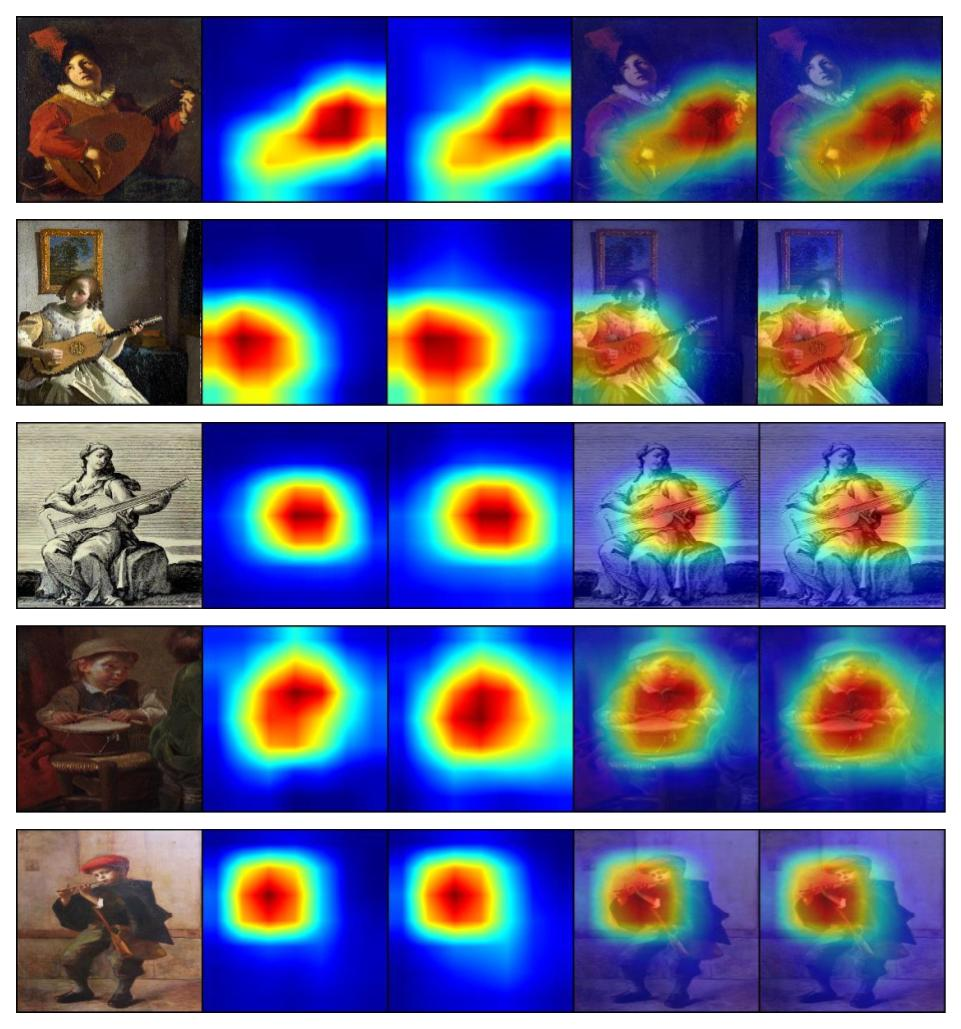
\includegraphics[width=\linewidth]{./Images/Chapter05/grad_cams}
  \caption{Saliency maps obtained after fine-tuning an ImageNet pre-trained ResNet50 on the \texttt{Minerva-Hypernym} benchmark. The first image corresponds to the original image, while the second and fourth images, and the third and fifth images, respectively report the performance of the Grad-CAM and Grad-CAM ++ methods.}
  \label{fig:grad_cams}
\end{figure}


\paragraph{\textbf{\uppercase{O}bject \uppercase{D}etection}}
Regarding the models trained for object detection, we visually investigate the quality of the predictions on the IconArt dataset \cite{gonthier2018weakly}, a database of $\approx 6000$ paintings that have been collected with the aim of detecting classes that are specific to the analysis of artworks. Among such classes, IconArt tackles the detection of ``angels'', ``Jesus'' and ``Mary'', or more simply ``ruins''. IconArt however, does not come with any ground truth labels that are suitable for the task of instruments detection, as the dataset has been built for different purposes. Yet, musical instruments might still be depicted within its images, and trying to detect them corresponds to a nice proof of concept that can show the benefits of deploying MINERVA pre-trained models to different artistic collections. In Fig. \ref{fig:wikiart_detections} we show some successful examples of detections that were obtained after testing the performance of a YOLO-V3 model that was fine-tuned on the \texttt{Minerva-Hypernym} benchmark. We see that the model can successfully detect musical instruments within this new artistic collection, a result that can be exploited by art historians interested in the study of musical instruments.   

\begin{figure}[ht!]
\centering
  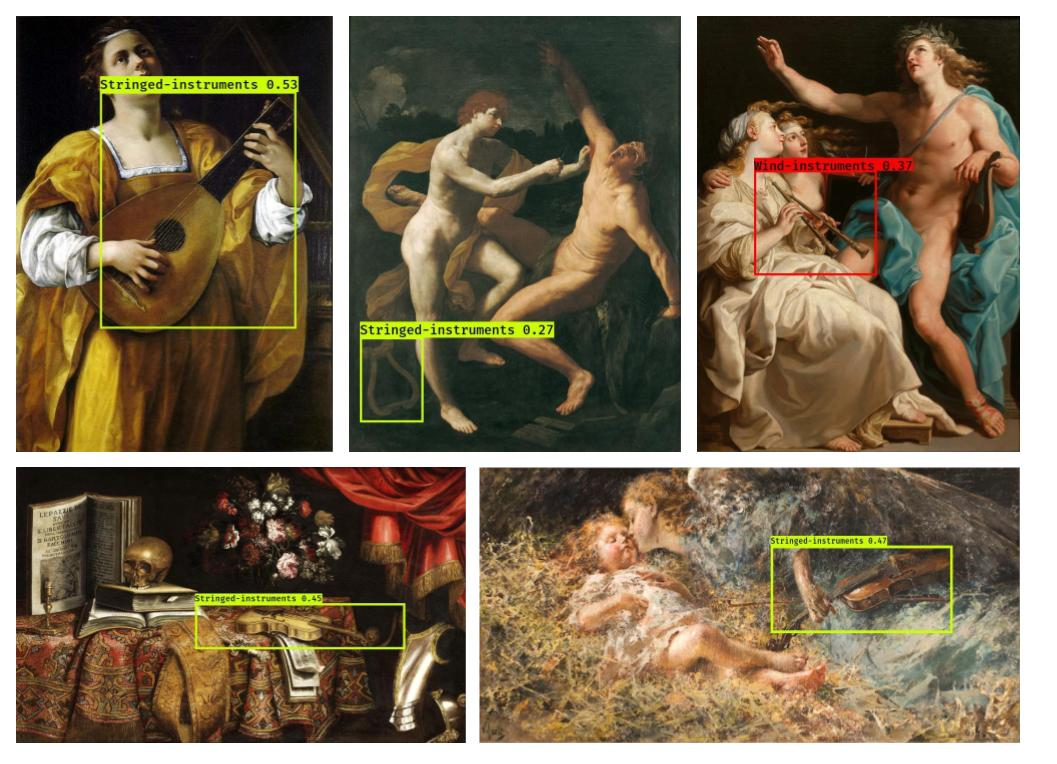
\includegraphics[width=\linewidth]{./Images/Chapter05/wikiart_detections}
  \caption{Some examples of successful detections that have been obtained on the IconArt dataset with a model fine-tuned on the \texttt{Minerva-Hypernym} benchmark.}
  \label{fig:wikiart_detections}
\end{figure}

While these results are undoubtedly nice and encouraging, it is arguably of even more considerable interest analyzing the model's erroneous detections. To this end, we have manually identified the incorrect predictions and grouped them into different categories. This process resulted in novel insights that, at least in part, explain the performance of the models that we have quantitatively assessed in Sec. \ref{sec:quantitative_analysis}.
First and foremost, we have noticed that the model strongly gravitates towards the detection of ``stringed instruments'' (a result which was already observed in Fig. \ref{fig:detection_experiment_2}) and that naturally stems from the fact that, as also presented in Fig. \ref{fig:hypernym_distribution}, stringed instruments are by far the most occurring type of instruments within MINERVA. However, we also believe that there are two more reasons which drive such erroneous detections: the significant presence of dual, conic contour curves of naked women's bodies, which are reminiscent of the resonance box of guitar-like instruments (see Fig. \ref{fig:false_positives_1}), and the presence of book-like objects that, just as instruments, are mostly depicted next to hands and fingers (see Fig. \ref{fig:false_positives_4}). We have then also observed that long, often martial objects such as swords, arrows, and spears are mistakenly detected as ``wind instruments''. We believe that the reason for this is that the shape between such objects and the one of instruments like ``shawns'', is very similar, and sometimes even hard to distinguish for the human eye (see Fig. \ref{fig:false_positives_2}).
Lastly, we have noticed that musical instruments are often mistakenly detected when regular patterns or parallel grids of straight lines (e.g. folds in clothing or wheel spokes) are present within the images. We hypothesize that the model associates these patterns to the presence of strings (see Fig. \ref{fig:false_positives_3}) within stringed instruments. 

\begin{figure}[ht!]
\centering
  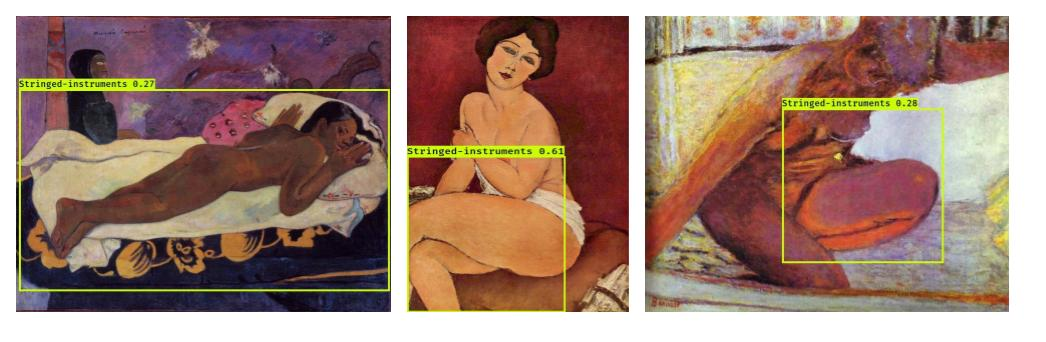
\includegraphics[width=\linewidth]{./Images/Chapter05/false_positives_1}
  \caption{Examples of false detections of ``stringed instruments'' within some images representing ``nudity'' that are part of the IconArt dataset.}
  \label{fig:false_positives_1}
\end{figure}

\begin{figure}[ht!]
\centering
  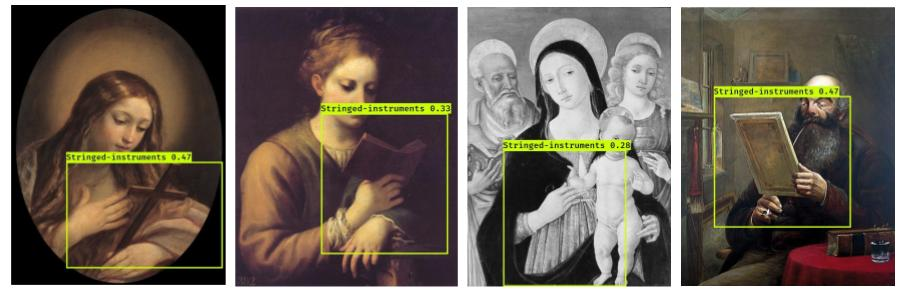
\includegraphics[width=\linewidth]{./Images/Chapter05/false_positives_4}
  \caption{Additional examples of false detections of ``stringed instruments'' that are triggered by the presence of objects close to hands and fingers.}
  \label{fig:false_positives_4}
\end{figure}

\begin{figure}[ht!]
\centering
  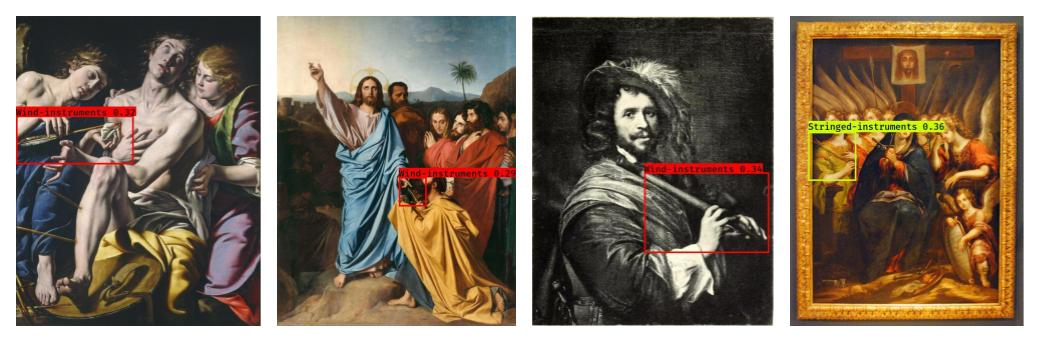
\includegraphics[width=\linewidth]{./Images/Chapter05/false_positives_2}
  \caption{Examples of false detections that are due to the strong resemblance between long martial objects and (mostly) ``wind instruments''.}
  \label{fig:false_positives_2}
\end{figure}


\begin{figure}[ht!]
\centering
  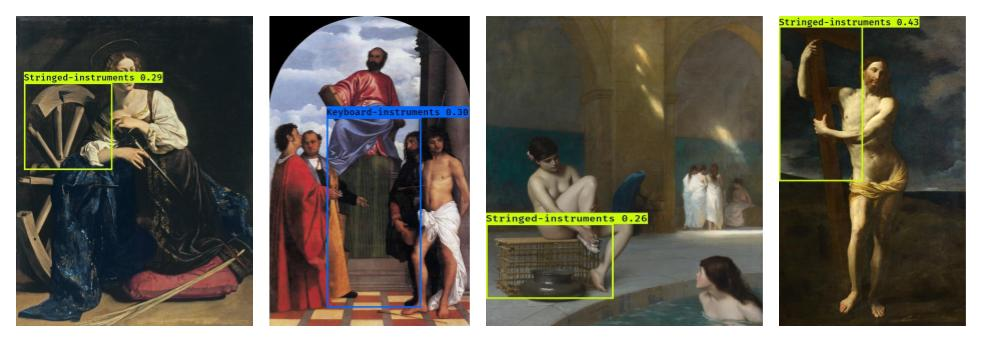
\includegraphics[width=\linewidth]{./Images/Chapter05/false_positives_3}
  \caption{Examples of geometrical patterns that mistakenly yield the detection of instruments.}
  \label{fig:false_positives_3}
\end{figure}



\section{Discussion and Critical Analysis}
\label{sec:discussion}
In this chapter, we have introduced MINERVA, the first sizable benchmark dataset for identifying and detecting musical instruments in unrestricted, digitized images from the realm of the visual arts. We hope that this dataset can serve as a novel test-bed for the computer vision community as it provides, at least in part, a solution to some of the challenges that currently define the field (see Sec. \ref{sec:cv_challenges}). Our benchmark experiments have highlighted the feasibility of our newly proposed classification and object detection tasks and served us for further characterizing the degree of transferability of pre-trained convolutional neural networks. While, when it comes to the classification experiments presented in the first part of Sec. \ref{sec:quantitative_analysis}, the obtained results are lower in terms of accuracy when compared to the classification tasks that we tackled in the previous chapter, they nevertheless provide strong evidence in favor of adapting transfer learning. At the same time, these experiments also show how challenging the simple task of image classification can be, as we believe there is definitively room for improving the results presented in Tables \ref{table:minerva_tl_results} and \ref{table:minerva_rijks_results}. Similarly, the results presented in the second part of Sec. \ref{sec:quantitative_analysis} show that it is equally possible to transfer models that have been initially built for the detection of objects in natural images and to use them on non-natural image distributions. We again believe that albeit satisfying results on MINERVA have been obtained by starting with an MS-COCO weight initialization, better performance than the one reported in Tables \ref{table:minerva_detection_hypernyms}, \ref{table:minerva_5_detection} and \ref{table:minerva_10_detection} can be obtained. To this end, we recommend taking into account the qualitative analysis that we presented in Sec. \ref{sec:qualitative_analysis}. Overall, our study is a first step towards creating novel, arguably more challenging computer vision test-beds that we hope can be used to further characterize the potential, and limitations, of modern state-of-the-art neural networks. To this end, the methodological protocol that was used for the creation of MINERVA has already inspired the development of new datasets and experimental studies that will be briefly reviewed in the next section.

\section{Future Work: towards more benchmarks}
\label{sec:future_work}

The work of Claes \cite{claes2021deep} has taken inspiration from the process that has led to the development of MINERVA, and has used the \texttt{Cytomine} platform for the creation of a novel object detection dataset that tackles the problem of animals detection in paintings. The dataset, coming with $\approx 8000$ images distributed over $25$ different animals classes, has successfully been used for confirming some of the main results that we presented throughout this chapter. More specifically, the good transfer learning properties of object detectors have also been observed when using models that, differently from the aforementioned YOLO architecture, use region proposals and selective search techniques for identifying possible locations of objects of interest within images \cite{girshick2015fast}. Furthermore, this work also shows the potential benefits that could come from using feature extractors that instead of being pre-trained on natural images, as was the case for the YOLO network used throughout this study, are pre-trained on artistic collections instead. Their study, which is in large part inspired by the research that we have performed at the end of the previous chapter also shows that the closer the source domain $\mathcal{D}_S$ and the target domain $\mathcal{D}_T$, the better the performance of a transferred model, therefore confirming some of the conclusions that we had drawn for image classification and generalizing them to object detection problems. We report some of the successful detections of animals in artworks obtained by Claes in Fig. \ref{fig:animals}.

\begin{figure}[ht!]
\centering
  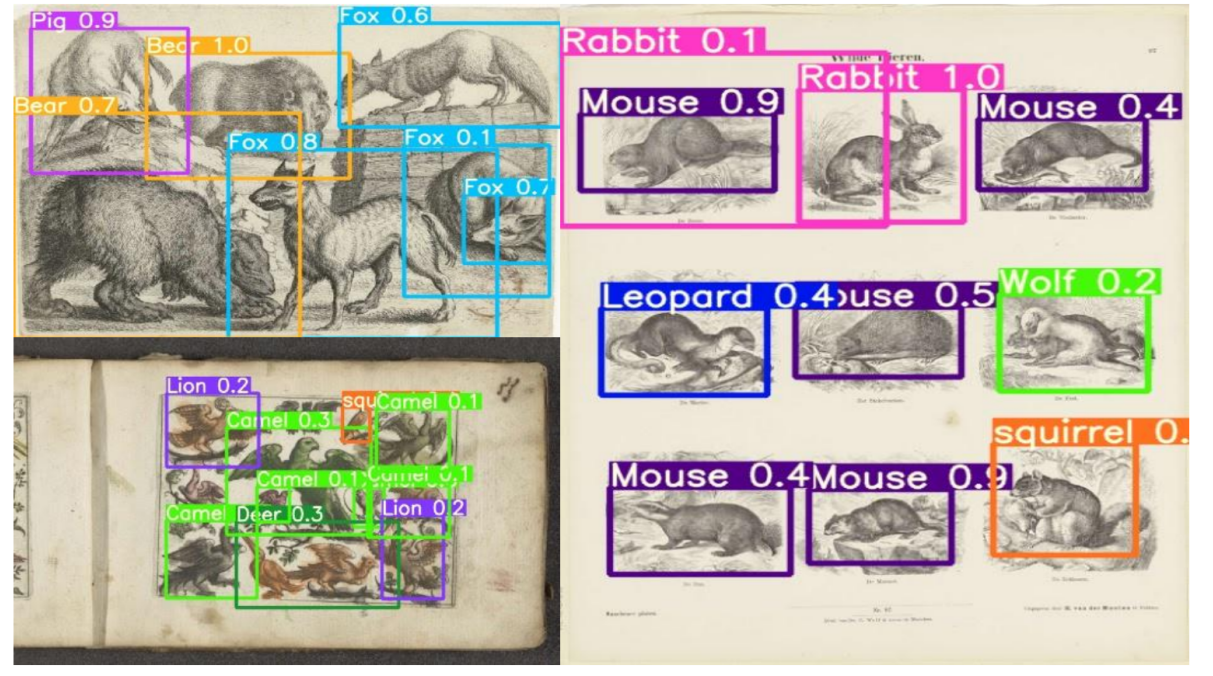
\includegraphics[width=\linewidth]{./Images/Chapter05/yann_animals.jpg}
  \caption{Some examples of animal detections within artworks obtained by Claes \cite{claes2021deep}.}
  \label{fig:animals}
\end{figure}

To conclude, we hope that MINERVA, together with the dataset created and benchmarked by \citet{claes2021deep} will push the Computer Vision community towards better identifying the transfer learning properties of convolutional neural networks. Furthermore, we also hope that the \texttt{Cytomine} platform, that was so successfully used for creating the aforementioned datasets, will in the future be used for developing novel datasets outside from the digital heritage and digital pathology domains.

 % DH Journal paper
\chapter{Reinforcement Learning and Deep Neural Networks}
\label{ch:reinforcement_learning}


\begin{remark}{Outline}

\end{remark}

\section{Introduction}
\label{sec:rl_introduction}


\section{Markov Decision Processes}
\label{sec:mdps}

In order to develop and apply RL algorithms to optimal decision making problems, we need to formulate the problem in a specific framework: in RL this is done with Markov Decision Processes (MDPs) \cite{puterman1990markov,puterman2014markov}. Throughout this thesis we will characterize MDPs, and the resulting RL concepts, by using the mathematical notation that was used by \citet{sutton2018reinforcement} in their seminal book about RL, although it is worth noting that within the literature, different formulations can be found to express the same kind of concepts \cite{bertsekas1995neuro,busoniu2010reinforcement,bertsekas2000dynamic,bertsekas2019reinforcement}.

We start by introducing the following elements:
\begin{itemize}
	\item A set of possible states $\mathcal{S}$, that can be visited by an agent while it is interacting with the MDP, where $s_t \in \mathcal{S}$ denotes the state being visited at time-step $t$.
	\item A set of possible actions $\mathcal{A}$ that are available to the agent when it is in a certain state, where $a_t \in \mathcal{A}(s_t)$ denotes the action that is performed by the agent in state $s$ at time-step $t$.
\item A transition function $\mathcal{P}:\matchal{S}\times\matchal{A}\times\matchal{S}\Rightarrow [0,1]$ that defines the probability for an agent to visit state $s_{t+1}$, based on its current state and the action which will be performed thereafter.
\item A reward function $\Re:\matchal{S}\times\matchal{A}\times\matchal{S}\Rightarrow \mathbb{R}$ which returns a reward signal $r_{t+1}$ when an agent performs action $a_t$ in state $s_t$ and transits to $s_{t+1}$.
\item A discount factor denoted as $\gamma \in [0,1]$.

\end{itemize}

Based on these concepts a MDP is then defined by the following tuple $<\mathcal{S}, \matchcal{A}, \matchal{P}, r, \gamma>$ and is also commonly denoted in the RL literature as the \textcolor{RoyalBlue}{environment}. The way the agent interacts with this environment is given by its \textcolor{RoyalBlue}{policy} $\pi$, defined as a probability distribution over $a \in \matchal{A}(s)$ for each $s \in \mathcal{S}$:
\begin{equation}
	\pi(a|s) = \text{Pr}\; \{A_t = a | S_t = s\}, \; \text{for all}\; s \in \mathcal{S}\; \text{and}\; a\ \in \mathcal{A}. 
\end{equation}
A policy can be deterministic if $\forall s:\pi(s,a) = 1$ for exactly one $a \in \mathcal{A}(s)$ and $\pi(s,b)=0$ for all other $b \in \mathcal{A}(s)$, while it is stationary if it does not change over time. In both cases the goal of a policy is to map each state to an action and is defined as: $\pi:\mathcal{S}\Rightarrow\mathcal{A}$.

The elements of a MDP allow us to properly model the dynamics of an agent interacting with its environment, an interaction which can be summarized as follows: at each time-step $t$ the environment provides the agent with a certain state $s_t$, the agent then performs action $a_t$ which results into the reward signal $r_{t+1}$. After performing such action the agent will enter into a new state $s_{t+1}$. This continuous interaction with the environment is also known as the Reinforcement Learning loop, and can technically be infinite. This is however never the case in practice, since an agent will eventually visit a state which only transits to itself (denoted as terminal), which will therefore stop the agent-environment interaction. We visually represent the Reinforcement Learning loop in Fig. \ref{fig:rl_loop}.

\begin{figure}[ht!]
\centering
  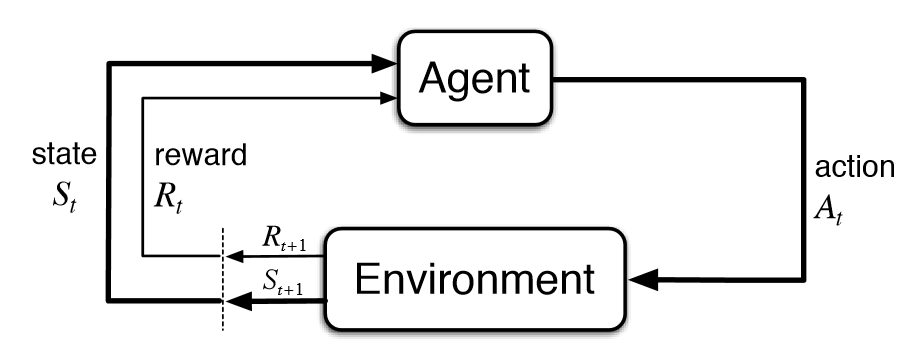
\includegraphics[width=10cm]{./Images/Chapter06/rl_loop.png}
  \caption{A visual representation of how an agent interacts with an environment as modeled by a Markov decision process. Figure taken from page 48 of the \citet{sutton2018reinforcement} textbook.}
  \label{fig:rl_loop}
\end{figure}

Each interaction of the agent with the environment is defined as an \textcolor{RoyalBlue}{episode}, which consists of one, or several trajectories $\tau$, that come in the form of the following sequence:
\begin{align}
	\langle(s_t,a_t,r_t,s_{t+1})\rangle,t=0,\ldots,T-1
\end{align}
where $T$ is a random variable representing the length of the episode.

A key property of the environment is that it fulfills the Markov property which is defined as follows:
\begin{definition}
	A discrete stochastic process is Markovian if the conditional distribution of the next state of the process only depends from the current state of the process.
\end{definition}
This implies that the only information that is necessary for predicting to which state an agent will step next are $s_t$ and $a_t$, which can be expressed formally as:
\begin{align}
	p(s_{t+1}|s_t, a_t, s_{t-1}, a_{t-1}, \ldots) = p(s_{t+1} | s_t, a_t).
\end{align}
Interestingly, a similar conclusion also holds for the reward that the agent will get, meaning that the reward that is obtained by an agent is only determined by its previous action, and not by the history of all previously taken actions, as defined by:
\begin{align}
	(r_t| s_t, a_t, \ldots, s_1, a_1) = p(r_t|s_t,a_t).
\end{align}


\section{Goals and Returns}
So far we have defined all the elements that model the interaction of an agent with an environment, whilst introducing some key properties that are key for the development of RL algorithms. While it is true that we have defined how the agent-environment interaction works, we yet do not know what the purpose of this interaction is. In RL the goal of an agent is defined with respect to the reward signal $r_t$ that is returned by the reward function $\Re$. Informally, the goal of an agent is that of maximizing the total amount of reward it receives while interacting with the environment. In the simplest case we can define this as:
\begin{align}
	G_t = r_t, r_{t+1}, r_{t+2}, \ldots, r_{T}.
\label{eq:goal}
\end{align}
While simple and intuitive this formulation has one major drawback: it treats each reward signal equally since it does not distinguish rewards that are obtained in the near future, i.e. $r_t$, from the ones that will be obtained in the more distant future, i.e. $r_{T-1}$. To deal with such issue we need an additional concept known as \textcolor{RoyalBlue}{discounting}, which can be governed by the discount rate parameter $\gamma$, also known as the discount factor. $\gamma$ allows us to weight the different reward signals based on how close or distant in the future these rewards are received by the agent. By introducing $\gamma$ in Eq. \ref{eq:goal} we can now define the expected discounted return as:
\begin{align}
	G_t & = r_t+\gamma r_{t+1}, \gamma^{2} r_{t+2} + ... \\
	    & = \sum_{k=0}^{\infty}\gamma^{k} r_{t+k+1}.
\label{eq:discounted_return}
\end{align}
The role of $\gamma$ can be interpreted as follows: a reward obtained $k$ time steps in the future is only worth $\gamma^{k-1}$ times what it would be worth if received immediately. It is easy to see how different $\gamma$ values can result into different agent's behaviors. If $\gamma=0$ an agent will only take into account immediate rewards, therefore aiming to maximize $r_{t+1}$ only and resulting into having a ``myopic" behavior. If $\gamma$ approaches $1$ the agent will become more ``far-sighted", it will take future rewards into account more strongly and will therefore increase its chances of accessing future rewards that will result into a higher cumulative return. 
Please note that by defining $\gamma \leq 1$ we can make the infinite sum presented in Eq. \ref{eq:discounted_return} finite as long as the sequence of rewards $r_k$ is bounded.   

While the role of $\gamma$ is often taken for granted within the RL literature it is worth noting that as mentioned by \citet{van2011insights} and \citet{schmidhuber2019reinforcement}, $\gamma$ is an artificial concept which is not present in fields such as traditional control theory or engineering. The reason of this is that $\gamma$ corresponds to a concept that does not exists in the real world, and that in practice distorts the real value of $r_t$ in an exponentially shrinking fashion. Even if it is considered common practice to include a discount factor in the development of RL algorithms, it is worth noting that making $\gamma$ part of the RL framework corresponds to including a form of ``inductive bias" within the resulting algorithms. It is common knowledge that low discount factors result into poor performance, and that it is therefore as beneficial as possible to set $\gamma$ as close to $1$, yet choosing an appropriate $\gamma$ parameter can be more challenging than expected especially when RL algorithms are combined with function approximators. \citet{wiering2009qv} show that different algorithms prefer different discount factors, while \citet{franccois2015discount} show the relationship between low discount factors and the values of the learning rate. Finally \citet{van2019using} introduce a method that allows the use of low discount factors for approximate RL algorithms, while at the same time highlighting that the common perception of the role of $\gamma$ might need revision from the RL community.             

\section{Value Functions}
We are now ready to introduce the arguably most important concept that underlies many RL algorithms: the concept of \textcolor{RoyalBlue}{value}. We can define the value of a state $s$, as well as the value of a certain policy $\pi$ or of a certain action $a$, anyhow, independently from what we are considering the notion of value is always directly linked to the concept of expected discounted return defined in Eq. \ref{eq:discounted_return}. Given an MDP and a policy $\pi$ we can determine the value of a state $s$ as a function that measures the expected return that the agent will receive when starting in $s$ and following $\pi$ thereafter. 
\begin{align}
    V^{\pi}(s)=\mathds{E}\bigg[\sum_{k=0}^{\infty}\gamma^{k}r_{t+k}\bigg| s_t = s, \pi \bigg].
    \label{eq:state_value_function}
\end{align}
$V^{\pi}(s)$ is also known as the \textit{state-value function} and intuitively tells us how good or how bad it is for an agent to be in a certain state. While this function is only conditioned on the state that is being visited by the agent, we can also condition it on the actions that are taken by the agent, which will quantify how good or bad it is for the agent to take a certain action $a$ in a certain state. This function comes with the name of \textit{state-action value function} and is defined as follows:
\begin{align}
     Q^{\pi}(s,a)=\mathds{E}\bigg[\sum_{k=0}^{\infty}\gamma^{k}r_{t+k} \bigg| s_t = s, a_t=a, \pi\bigg].
 \end{align}
Both value functions are very powerful since they allow us to characterize the behavior of an agent by quantitatively assessing its interaction with the environment. They can be seen as the knowledge of the agent and represent its desirability of being in a specific state. As we will see in the coming sections, accurately modeling these value functions is one of the major goals of RL.  

A key property of $V^{\pi}(s)$ and $Q^{\pi}(s,a)$ is that both value functions satisfy a consistency condition that allows us to define both functions recursively. For example let us consider the state-value function $V^{\pi}(s)$ presented in Eq. \ref{eq:state_value_function}, we can rewrite it as:
\begin{align}
 V^{\pi}(s) & =\mathds{E}\big[\sum_{k=0}^{\infty}\gamma^{k}r_{t+k}\big| s_t = s, \pi \big] \\ 
 & =\mathds{E}\big[r_{t+1}+\gamma r_{t+2}+\gamma^{2}r_{t+3}+\ldots \big| s_t =s , \pi \big] \\ 
 & =\mathds{E}\big[r_{t+1}+\gamma(r_{t+2}+\gamma r_{t+3}+\ldots)\big| s_t =s , \pi \big] \\
 & =\mathds{E}\big[r_{t+1}+\gamma V^{\pi}(s_{t+1}) \big| s_t =s , \pi \big] \\
 & =\sum_a \pi(s,a) \sum_{s+1} p(s_{t+1}|s,a)\big[\Re(s_t, a, s_{t+1}) + \gamma V^{\pi}(s_{t+1}) \big].
\end{align}
Similar steps can be followed when considering $Q^{\pi}(s,a)$ which can then be recursively defined as:
\begin{equation}
	Q^{\pi}(s,a) = \sum_{s_{t+1}} p(s_{t+1}|s,a)\big(\Re(s_t, a, s_{t+1}) + \\ \gamma \sum_{a_{t+1}} \pi(s_{t+1},a_{t+1}) Q^{\pi}(s_{t+1}, a_{t+1}) \big).
\end{equation}

When it comes to sequential decision making, we are interested in maximizing the value of each state or of each state-action pair, since by doing so we will be finding a policy $\pi$ that is optimal. The \textcolor{RoyalBlue}{optimal policy} $\pi^{*}$ is a policy that realizes the optimal expected return defined as:
\begin{align}
 V^{*}(s)=\underset{\pi}{\max}\:V^{\pi}(s), \ \text{for all} \ s\in\mathcal{S}
\end{align}
and the optimal $Q$ value function:
\begin{align}
Q^{*}(s,a)= \underset{\pi}{\max}\:Q^{\pi}(s,a) \ \text{for all} \ s\in\mathcal{S} \ \text{and} \ a \in\mathcal{    A}.
\end{align}
When we recursively define both optimal value functions as we did for Eq. \ref{eq:state_value_function} we obtain:
\begin{align}
    V^{*}(s_t) = \underset{a}{\max}\sum_{s_{t+1}}p(s_{t+1} | s_{t}, a) \bigg[\Re (s_{t}, a, s_{t+1}) + \gamma V^{*}(s_{t+1}) \bigg]
    \label{eq:optimal_v}
\end{align}
and
\begin{multline}
    Q^{*}(s_t,a_t)=\sum_{s_{t+1}}p(s_{t+1} | s_{t}, a_{t})  \bigg[\Re (s_{t}, a_{t}, s_{t+1}) + \gamma \: \underset{a}{\max} \: Q^{*}(s_{t+1}, a) \bigg],
    \label{eq:optimal_q}
\end{multline}
which are well known to correspond to the Bellman \textcolor{RoyalBlue}{optimality} equations \cite{bellman1966dynamic}. 

If the optimal $Q$ function is learned it becomes as straightforward task to derive an optimal policy since one only needs to select the action which has the highest value in each state as defined by:
\begin{equation}
	\pi^{*}(s) = \underset{a\in\mathcal{A}}{\argmax} \ Q^{*}(s,a) \ \text{for all} \ s \in \mathcal{S}.
\end{equation}

It is also worth noting that the $Q$ function and the $V$ function satisfy the following equality
\begin{align}
	V^{*}(s) = \underset{a\in\mathcal{A}}{\max} \ Q^{*}(s,a) \ \text{for all} \ s \in \mathcal{S}
\end{align}
which comes from the fact $V^{*}(s) \leq \max_{a\in\mathcal{A}} \ \text{for all} \ s\in\mathcal{S}$. As we will later see throughout this thesis this equality is particularly important for the development of many RL algorithms.


\section{Learning Value Functions}
The $V$ function and the $Q$ function play a crucial role when it comes to the development of optimal decision making algorithms, and over the years several methods have been introduced to learn them. While the ultimate goal of all these algorithms is that of yielding an optimal policy, there exists cases for which learning these value functions are easier than others. The complexity of learning a value function depends from how many components of the MDP are known to the agent. If the agent has access to all five of the components of the MDP that we introduced in Sec. \ref{sec:mdps}, these algorithms are part of a collection of methods that comes with the name of \textcolor{RoyalBlue}{Dynamic Programming} (DP). DP algorithms such as \textit{value-iteration}, \textit{policy-iteration} and variants \cite{bertsekas2015value,wei2015value} learn an optimal value function or optimal policy by exploiting the fact that the transition function $\matchcal{P}$, and the reward function $\Re$ of the MDP are known. While DP methods can be considered as the progenitors of many RL algorithms we will not discuss them here since throughout this thesis we will be interested in scenarios for which $\matchal{P}$ and $\Re$ are unknown. Specifically, we will introduce novel methods that aim to learn an optimal value function without requiring to learn an approximation of the transition and reward functions ($\widehat{\matchal{P}}$ and $\widehat{\mathcal{\Re}}$) neither, therefore placing all contributions of this dissertation within the \textcolor{RoyalBlue}{model-free} RL literature. 

\subsection{Monte Carlo Methods}
The first family of methods that is able of learning optimal value functions when no complete knowledge of the environment is available comes with the name of Monte Carlo (MC) methods. MC algorithms only require RL trajectories in order to discover an optimal policy and achieve this by sampling and averaging the rewards that are obtained while the agent is interacting with the environment. While MC methods can be used both for learning $V^{*}(s)$ and for learning $Q^{*}(s,a)$, in this section we only present how one can learn the state-value function. The key idea of MC algorithms relies on computing the actual sum of discounted rewards that an agent obtains once an episode finishes, this corresponds to computing the quantity defined in Eq. \ref{eq:goal}. Once this value is computed it can be used for updating the current value of each state with the following update rule: 
\begin{equation}
	V(s_t) := V(s_t) + \alpha \big[G_t - V(s_t) \big]
\label{eq:mc_update}
\end{equation}
where $\alpha \in [0,1]$ is the learning rate controlling how much we want to change the value estimate of a state based on $G_t$. As a practical example let us consider the MDP represented in Fig. \ref{fig:mdp}. Let us assume that the starting state of the environment is $s_0$ while the terminal state of the environment is $s_2$, and that the agent follows a policy $\pi$ that results into actions $a_1, a_2$ and $a_3$. The rewards associated to each action are: $-1, +2$ and $+3$ respectively. If we set the discount factor to $0.99$ we know that the real discounted return that is obtained at the end of the agent-environment interaction when starting in state $s_0$ is $\sum_{k=0}^{\infty}\gamma^{k} r_{t+k+1} = -1+\gamma2+\gamma^{2}3 \approx 3.92$. If we assume that the current value of $s_0$ before is $0$, and that we set $\alpha=0.5$, the result of one MC update for $s_0$ will be $\approx 1.96$.    

When dealing with MC learning it can however be possible that a certain state is visited more than once before a terminal state is reached. This is the case for $s_0$ for the MDP represented in Fig. \ref{fig:mdp}. If that happens one must decide when to update $V(s)$ and which value to use as $G_t$ since different state visits result into different $G_t$ values. There are two typical ways to deal with this, one can either update $V(s)$ only once, or one can update $V(s)$ each time the state is visited by simply using as $G_t$ the average of all the different discounted returns. The first update strategy comes with the name of , while the latter is denoted as .

\begin{figure}[ht]
	\centering
	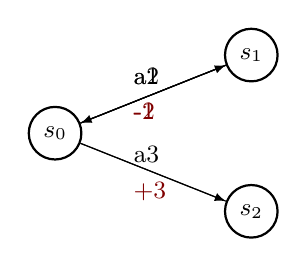
\begin{tikzpicture}[auto,node distance=8mm,>=latex,font=\small]

    \tikzstyle{round}=[thick,draw=black,circle]

    \node[round] (s0) {$s_0$};
    \node[round,above right=5mm and 20mm of s0] (s1) {$s_1$};
    \node[round,below right=5mm and 20mm of s0] (s2) {$s_2$};

    \draw[->] (s0) -- node [text width=0.5cm,above] {a1} (s1);
    \draw[] (s0) -- node [text width=.5cm,below] {\textcolor{Maroon}{-1}} (s1);

    \draw[->] (s0) -- node [text width=0.5cm,above]{a3} (s2);
    \draw[] (s0) -- node [text width=.5cm,below] {\textcolor{Maroon}{+3}} (s2);

    \draw[->] (s1) -- node [text width=0.5cm,above]{a2} (s0);
    \draw[] (s1) -- node [text width=.5cm,below] {\textcolor{Maroon}{-2}} (s0);

\end{tikzpicture}
\caption{A visual representation of a simple MDP.}
\label{fig:mdp}
\end{figure}

While several successful applications of MC methods exist \cite{jaakkola1995reinforcement,liu1998sequential,lazaric2007reinforcement}, a well known issue from this family of algorithms is that they suffer from highly biased updates. In fact one needs to compute the sum presented in Eq. \ref{eq:goal} over all visited states, which can result into returns with considerable variance. It is easy to see how this can become an issue especially when the length of the episodes increases since the larger the length of the episode, the larger the variance of the updates will be. Furthermore, an additional drawback of MC methods is that one must wait until the agent visits a terminal state before being able to perform an update that is based on Eq. \ref{eq:mc_update}, the latter drawback can result into slow learning and is addressed by the methods which will be presented hereafter.   

\subsection{Temporal Difference Learning}
\label{sec:td_learning}
Temporal Difference (TD) Learning \cite{sutton1984temporal,sutton1988learning} is a learning paradigm that allows to overcome the aforementioned issues that characterize MC learning based methods. The key idea of TD-Learning is to update the value of each state with respect to a single MC update, therefore overcoming the hurdle of having to wait for the end of an episode before being able to update the value of a state. Just as MC methods TD-Learning algorithms also learn an optimal value function simply based on the experience that is collected by the agent, however these algorithms base their updates only on the value of a single consecutive state rather than on the real discounted return that is dependent from the entire sequence of visited states. Updating the value of a state with respect to the value of its successor state only is a technique which comes with the name of \textcolor{RoyalBlue}{bootstrapping}, and is a very effective design choice that reduces the variance in the updates. Bootstrapping can be used both for learning the $V$ function and the $Q$ function and is at the core of the most popular model-free RL algorithms. The fist and simplest form of TD-Learning was introduced by \citet{sutton1988learning} for learning the state-value function with an algorithm that updates the value of a state based on the following learning rule:
\begin{equation}
	V(s_t):= V(s_t) + \alpha \big[r_t + \gamma V(s_{t+1}) - V(s_t)\big].
	\label{eq:td_learning_v}
\end{equation}
We can now clearly see that differently from what happens in the MC update presented in Eq. \ref{eq:mc_update} the update of a state now only depends from the reward and the value of the next state. This quantity is denoted as the TD-error $\delta_t$ and is defined as:
\begin{equation}
	\delta_t = r_t + \gamma V(s_{t+1}) - V(s_t).
\end{equation}
where $r_t + \gamma V(s_{t+1})$ is also known as the TD-target.
If we again consider the simple MDP represented in Fig. \ref{fig:mdp} and assume that the value of each state of the process is set to $0$ while the discount factor $\gamma$ is again set to $0.5$, a TD update for $V(s_0)$ based on action $a_3$ will result into the new value estimate of $1.5$. 
TD-Learning is a very effective strategy for building algorithms that can learn in an online, fully incremental fashion, since one only needs to wait a single time-step before being able to update the considered value function. Due to its striking simplicity TD-Learning has been widely adopted by RL practitioners developing algorithms for learning the $Q$ function. We will present some of the most important algorithms hereafter. 

\paragraph{Q-Learning:} introduced by \citet{watkins1992q} is arguably the most popular model-free RL algorithm. It works by keeping track of an estimate of the state-action value function $Q: \mathcal{S} \times \mathcal{A} \rightarrow \Re$ and updates each visited state-action pair with the following update rule:
\begin{equation}
Q(s_t,a_t):=Q(s_t,a_t) + \alpha\big[r_t + \gamma \underset{a\in \mathcal{A}}{\max} Q(s_{t+1},a_t) - Q(s_t, a_t) \big].
\label{eq:q_learning}
\end{equation}
The key component of Q-Learning's update rule is the $\max$ operator which characterizes its TD-error and that is necessary for constructing the TD-target. Since there are as many Q values as there are actions available to the agent, one must choose which Q value to use as a reference when updating the value of the state-action pair that is currently being visited by the agent. The $\max$ operator simply chooses the state-action pair with the largest Q value, a simple design choice that has the appealing property of making Q-Learning converge to $Q^{*}(s,a)$ with probability 1 as long as all state-action pairs are visited infinitely often. Interestingly this guarantee holds even if a random policy is followed by the agent. The $\max$ operator also defines Q-Learning as an \textcolor{RoyalBlue}{off-policy} learning algorithm, since the Q values chosen for the construction of the TD-target might not correspond to the ones that are associated to the state that will be visited by the agent after having updated its $Q$ function.

\paragraph{SARSA:} also known as `online Q-Learning" \cite{rummery1994line} can be seen as the most straightforward extension of the TD-Learning method presented in Eq. \ref{eq:td_learning_v}, and similarly to Q-Learning is an algorithm that aims at learning the state-action value function $Q$. The key idea of SARSA is to update a state-action value with respect to the Q value that is associated to the state that will be visited by the agent after a certain action is performed. SARSA does therefore not use the $\max$ operator within its TD-error and constructs TD-targets that are representative of the policy that is being followed by the agent, a characteristic that defines SARSA as an \textcolor{RoyalBlue}{on-policy} RL algorithm. The way SARSA learns the $Q$ function is given by the following update rule
\begin{equation}
	Q(s_t,a_t):=Q(s_t,a_t) + \alpha\big[r_t + \gamma Q(s_{t+1},a_{t+1}) - Q(s_t, a_t) \big], 
	\label{eq:sarsa}
\end{equation}
where we can clearly see how the algorithm uses all the elements of the quintuple of events $(s_t, a_t, r_t, s_{t+1}, a_{t+1})$ a property that gives rise to the name $sarsa$. Not using the $\max$ operator in Eq. \ref{eq:sarsa} results into an algorithm that differently from Q-Learning does not directly learn the optimal $Q$ function anymore, but rather learns to estimate $Q^{\pi}(s,a)$. This has the drawback of not guaranteeing convergence to $Q^{*}(s,a)$ for any random policy anymore. To overcome this SARSA needs an exploration policy that is greedy in the limit of infinite exploration \cite{singh2000convergence}. This can be achieved with the popular $\epsilon-\text{greedy}$ selection policy which defines the action that is taken by the agent as:
\begin{equation}
a_t = \begin{cases}
\underset{a\in\mathcal{A}}{\argmax} \ Q(s_t,a) &\text{with probability $1-\epsilon$}\\
a \sim \mathcal{U}(\mathcal{A}) &\text{with probability $\epsilon$}
\end{cases}
\label{eq:e_greedy}
\end{equation}
where $\epsilon$ is a hyperparameter that changes while training progresses. During early training iterations its value is close to $1$, while it approaches $0$ by the end of training. This allows the agent to take actions that are representative of a large set of policies when the learned $Q$ function does not yet correspond to $Q^{*}(s,a)$, while it will favor greedy actions at the end of training. This is a simple, yet effective strategy to deal with the \textcolor{RoyalBlue}{exploration-exploitation} dilemma and it is worth noting that its use is not limited to on-policy RL algorithms only. Furthermore the method presented in Eq. \ref{eq:e_greedy} represents only one possible way of balancing exploration and exploitation, and although it is arguably the most popular of such methods it is not the only existing one. We refer the reader to chapter 5 of \cite{wiering1999explorations} for a thorough analysis of different exploration algorithms.


\paragraph{Double Q-Learning:}


\paragraph{QV($\lambda$)-Learning:} first introduced by \citet{wiering2005qv} and further developed by \citet{wiering2009qv} is an on-policy RL algorithm which differently from the previously introduced methods keeps track of an estimate of the state-value function $V:\mathcal{S}\rightarrow\Re$ alongside the usual estimate of the state-action value function $Q:\mathcal{S}\times\mathcal{A}\rightarrow\Re$. Since the goal is that of jointly learning two value functions, QV($\lambda$)-Learning requires two separate update rules. The $V$ function is learned via the same form of TD-Learning that we introduced in Eq. \ref{eq:td_learning_v}, with the only difference being the addition of the eligibility traces $e_t(s)$ at the end of the update rule (a RL technique that we will not discuss in this dissertation). QV($\lambda$)-Learning therefore learns the $V$ function with the following update rule:
\begin{equation}
V(s):= V(s) + \alpha \big[ r_{t} + \gamma V(s_{t+1}) - V(s_t) \big] e_{t}(s).
\label{eq:qv_lambda_v_update}
\end{equation}
Since as discussed earlier only learning the $V$ function is not sufficient for deriving an optimal policy one needs to learn the $Q$ function as well. In QV($\lambda$)-Learning this is done as follows:
\begin{equation}
Q(s_{t}, a_{t}):= Q(s_{t}, a_{t}) + \alpha \big[r_{t} + \gamma V(s_{t+1}) - Q(s_{t}, a_{t}) \big].
\label{eq:qv_lambda_q_update}
\end{equation}
An interesting property of the algorithm is that it uses the same TD-target ($r_t + \gamma V(s_{t+1})$) for defining the two different TD-errors that are required for learning the state-value and the state-action value functions. Among the main insights which motivate learning two value functions over one \citet{wiering2005qv} mentions the possibility that the $V$ function, since it does not depend from the actions that are taken by the agent, might converge faster than the $Q$ function. In fact as described earlier, the $V$ function only depends from the state space of the MDP which by definition is smaller than the state-action space. For a more in-depth and formal presentation of the conditions that show the benefits of jointly learning the $V$ function alongside the $Q$ function we refer the reader to chapter 5 of \cite{van2011insights}.


\section{Function Approximators}
If it is true that model-free RL algorithms are very powerful methods for learning an optimal policy when parts of the MDP are unknown, it is also true that all the aforementioned algorithms suffer from the \textcolor{RoyalBlue}{curse of dimensionality}. Model-free algorithms are typically implemented in a tabular fashion, meaning that the state values, or state-action values, are stored within a table of sizes $|\matchal{S}|$ and $|\mathcal{S}\times\mathcal{A}|$ respectively. Albeit straightforward and easy to implement such an approach presents severe limitations. The first major drawback of the tabular representation approach is that it does not scale well with respect to the complexity of the MDP. If the state and action spaces of the environment become very large, storing a table quickly becomes unfeasible in terms of storage space. Furthermore tabular representations are also unable to deal with states that are continuous. A natural solution to this problem consists in discretizing the state space, which unfortunately, when done thoroughly, results into the same aforementioned storage space issues. A common solution that makes it possible to use RL techniques even when the state space of the MDP is large is based on parametrized function approximation. In this context the goal is to not learn the exact value function anymore, but to rather replace its tabular representation with a parametrized function. The parameters of this function can then be adjusted based on the RL algorithms that we introduced in Sec. \ref{sec:td_learning}. 


\subsection{Linear Functions}
\label{sec:linear_functions}

The most straightforward type of function approximator one can use is a linear function. Given a state-action tuple that gets represented as a feature vector $\vec{x}=[f_1(s,a), f_2(s,a), ..., f_i(s,a)] \in \mathds{R}^2$, and a function parametrized by a vector of parameters $\theta$, as shown in \cite{wiering2004convergence} we can redefine the value of a state-action pair as:
\begin{equation}
	Q(s,a) = \sum_i \theta_{i,a} \vec{x}_i(s).
\end{equation}
Given a trajectory $\langle s_t,a_t,r_t,s_{t+1}\rangle$ the Q-Learning algorithm presented in Eq. \ref{eq:dqn} can now be used for updating the parameters $\theta$ for all $i$ with the following update rule:
\begin{equation}
	\theta_{i,a_t} := \theta_{i,a_t} + \alpha(r_t +\gamma\underset{a\in \mathcal{A}}{\max} Q(s_{t+1},a_t) - Q(s_t, a_t)\vec{x}_i(s_t).
	\label{eq:q_learning_fa}
\end{equation}
We can observe that this update rule is equivalent to updating the parameter vector $\theta$ for minimizing the mean squared error loss between a given state-action tuple and Q-Learning's TD-target since  
\begin{align}
	& \mathcal{L}(\theta) = \frac{1}{2}\big(y_t - Q(s_t, a_t)\big)^2 \\ 
	& \frac{\partial\mathcal{L}}{\partial \theta_{i,a_t}}=-\big(y_t - Q(s_t, a_t)\big)\vec{x}_i(s_t)  \\ 
 	& \theta_{i,a_t} := \theta_{i,a_t} + \alpha(r_t +\gamma\underset{a\in \mathcal{A}}{\max} Q(s_{t+1},a_t) - Q(s_t, a_t)\vec{x}_i(s_t).
\end{align}

Similar steps can be used for adapting all the RL algorithms that we introduced in the previous section. As a representative example for the on-policy learning case let us consider the SARSA algorithm, which can be used for minimizing the parameters of a linear function as:
\begin{equation}
	\theta_{i,a_t} := \theta_{i,a_t} + \alpha(r_t +\gamma Q(s_{t+1},a_{t+1}) - Q(s_t, a_t)\vec{x}_i(s_t).
\end{equation}
Among the different functions one can use there are CMACs \cite{lane1992theory}, radial basis functions (RBFs) \cite{park1993approximation}, linear neural networks \cite{mcculloch1943logical} and linear support vector machines (SVMs). Although these techniques can be successfully used for dealing with the aforementioned curse of dimensionality problem, \textcolor{RoyalBlue}{non-linear} functions are usually preferred since their representational power is much larger than the one of linear methods. Throughout this dissertation we are interested in non-linear functions that come in the form of deep neural networks, which despite being able of learning rich representations from their inputs, are also particularly challenging to train when it comes to RL problems. We will now describe how one can successfully deal with some of the challenges that characterize the use of deep neural networks in RL by presenting some of the most important algorithms that have been introduced over the years.    

\subsection{Deep Neural Networks}
Before looking into how RL algorithms should be integrated within deep neural networks, it is important to mention that RL techniques have been successfully used in combination with (less powerful) neural networks for over three decades. In fact, the field known as \textcolor{RoyalBlue}{Connectionist Reinforcement Learning} (CRL) gave born to the very first algorithms that managed to outperform human experts on certain tasks. Among the possible multiple examples of this family of techniques we mention the TD-Gammon program introduced by \citet{tesauro1994td}. TD-Gammon successfully learns an approximation of the evaluation function of the popular Backgammon board-game through the same TD-Learning methods that we presented in Sec. \ref{sec:td_learning} and achieved a level of play which was comparable to the one of the top human Backgammon players of its time. For a more detailed presentation about the successful applications of CRL algorithms we refer the reader to \cite{bucsoniu2011approximate}.  

While certainly successful for a certain set of problems (see for example chapter $1$ of \cite{sabatelli2017learning}), CRL techniques also present severe limitations. Since they only use multi-layer perceptrons as function approximators, these algorithms cannot be used for tackling problems where the state representation of the MDP is highly dimensional. To overcome this, more complicated and powerful networks are required. \textcolor{RoyalBlue}{Deep Reinforcement Learning} (DRL) \cite{arulkumaran2017deep, li2017deep, franccois2018introduction} is a research field that combines RL algorithms with deeper and more complex neural architectures. In value based model-free DRL we are interested in learning an approximation of an optimal value function with a deep neural network that comes with parameters $\theta$

\noindent
\begin{tabularx}{\linewidth}{@{}XX@{}}
\begin{equation}
	  V(s;\theta)\approx V^{*}(s)
	  \label{eq:v_approx}
  \end{equation}
&
\begin{equation}  
	Q(s,a;\theta)\approx Q^{*}(s,a)
	\label{eq:q_approx}
  \end{equation}
\end{tabularx}
and that usually comes in the form of a convolutional neural network. We now report some of the most popular DRL algorithms. 


\paragraph{Deep Q-Learning (DQN):} just like Q-Learning is arguably the most important tabular model-free RL algorithm, so is DQN when it comes to DRL. First introduced by \citet{mnih2013playing} and then made popular by the work presented in \cite{mnih2015human} this algorithm can certainly be considered as the very first successful example of a neural network that is able to learn an approximation of the optimal state-action value function just from high sensory inputs such as images. As the name suggests, DQN is based upon the Q-Learning algorithm, and aims at learning an approximation of the optimal state-action value function $Q$. This is done by reshaping Q-Learning's update rule, presented in Eq. \ref{eq:q_learning}, into a differentiable loss function that can be used for training a convolutional network with the following objective function:
\begin{multline}
	\mathcal{L}(\theta) = \mathds{E}_{\langle s_{t},a_{t},r_{t},s_{t+1}\rangle\sim U(D)} \bigg[\big(r_{t} + \gamma \: \underset{a\in \mathcal{A}}{\max}\: Q(s_{t+1}, a; \theta^{-}) \\ - Q(s_{t}, a_{t}; \theta)\big)^{2}\bigg].
\label{eq:dqn}
\end{multline}

We can start by observing that the general principles that characterize the algorithm are the same ones which made it possible to generalize Q-Learning to the use of linear function approximators, although it is worth noting that differently from when a linear function is used the mapping between input and feature spaces is now not preserved anymore. Similarly to what we presented in Sec. \ref{sec:linear_functions}, we can see from Eq. \ref{eq:dqn} that learning $Q(s,a,\theta)$ is again achieved by minimizing the squared error loss between the $Q(s_t,a_t;\theta)$ estimates and the off-policy TD-target
\begin{equation}
    y^{DQN}_{t} = r_{t} + \gamma \: \underset{a\in \mathcal{A}}{\max}\: Q(s_{t+1}, a; \theta^{-}).
\label{eq:dqn_td}
\end{equation}
Despite this similarity DQN requires some additional algorithmic design choices, without which, it would result impossible to successfully train a neural network with Eq. \ref{eq:dqn}. These additions, which significantly make DQN differ from the algorithm presented in Eq. \ref{eq:q_learning_fa} are the following:
\begin{itemize}
	\item \textcolor{RoyalBlue}{Experience Replay}: a memory buffer, $D$, represented as a queue which stores RL trajectories of the form $\langle s_{t}$, $a_{t}$, $r_{t}$, $s_{t+1} \rangle$. Once this memory buffer is filled with a large set of these quadruples, DQN uniformly samples batches of trajectories for training its network. This makes it possible to exploit past trajectories multiple times by reusing them while training, which makes the overall algorithm more sample efficient. Furthermore, using a memory buffer also improves the stability of the training procedure. Recall that each trajectory is representative of a certain episode, by repeatedly randomly sampling a different $\tau$ from the memory buffer, a resulting mini-batch of trajectories will be representative of different episodes and of different policies. As a consequence the correlation between trajectories within a mini-batch will be small. Although made popular by the DQN algorithm, the use of an experience replay buffer for tackling optimal decision making problems was already presented by \citet{lin1992self}.
		
	\item \textcolor{RoyalBlue}{Target Network}: We can observe from Eq. \ref{eq:dqn_td} that the TD-target used by DQN for bootstrapping is not computed by the $Q$ network that is being optimized ($\theta$), but rather from a second separate network that is parameterized with $\theta^{-}$. This second network has the same structure as the main $Q$ network, but its weights do not change each time RL experiences are sampled from $D$. On the contrary, its weights are temporally frozen, and only periodically get updated with the parameters of the main network $\theta$ as defined by an appropriate hyperparameter. Note that this is a design choice that is not motivated by the TD-Learning paradigm that we presented in Sec. \ref{sec:td_learning}, where we have seen that TD-Learning based methods learn in a fully online fashion by updating their value estimates based on their own future estimates. With a target-network, although the $\theta$ network still learns via the methods of temporal differences, it now requires an auxiliary, external model if it wants to successfully learn $\approx Q^{*}(s,a;\theta)$. Several research has studied the role of the target network with the aim of understanding why this design choice appears to be necessary for DRL, yet the role of $\theta^{-}$ is not fully understood by the DRL community. For more about this topic we refer the reader to .

\end{itemize}

Now that all components of Eq. \ref{eq:dqn} are introduced we can show that given a training iteration $i$, differentiating this objective function with respect to $\theta$ gives the following gradient: 
\begin{multline}
\nabla_{\theta_{i}}y^{DQN}_{t}(\theta_{i}) = \mathds{E}_{\langle s_{t},a_{t},r_{t},s_{t+1}\rangle\sim U(D)} \bigg[\big(r_{t} + \\ \gamma \: \underset{a\in \mathcal{A}}{\max}\: Q(s_{t+1}, a; \theta^{-}_{i-1})  - Q(s_{t}, a_{t}; \theta_{i})\big)\nabla_{\theta_{i}} Q(s_{t}, a_{t}; \theta_{i})\bigg].
\label{eq:dqn_gradient}
\end{multline}

The DQN algorithm showcased its entire potential in \cite{mnih2015human} where Mnih and colleagues developed a convolutional neural network that trained with Eq. \ref{eq:dqn} learned how to successfully play most of the \texttt{Atari} games that are part of the popular Atari Arcade Learning Environment (ALE) \cite{bellemare2013arcade}, a well known platform that even nowadays serves as a benchmark when it comes to testing the performance of DRL algorithms. In the ALE a DRL algorithm has to learn how to play $57$ different emulations of \texttt{Atari} games which are specifically designed within a simulator (see Fig. \ref{fig:atari_games} for a visualization of some of the games that are part of the ALE suite). Remarkably, DQN learned not only learned how to play most of the games of the platform, but also achieved a final performance that, on most of games, was superior than the one of human expert players. What is even more remarkable is that this was achieved by providing as inputs to the network the images representing the game only, therefore making the model learn just from its own experience in a pure model-free RL fashion. Since then, DQN has been successfully used for a large variety of applications ranging from, to and .
However, despite all these remarkable applications the algorithm still comes with some drawbacks, some of which were solved by the algorithms presented below.

\begin{figure}[ht!]
\centering
  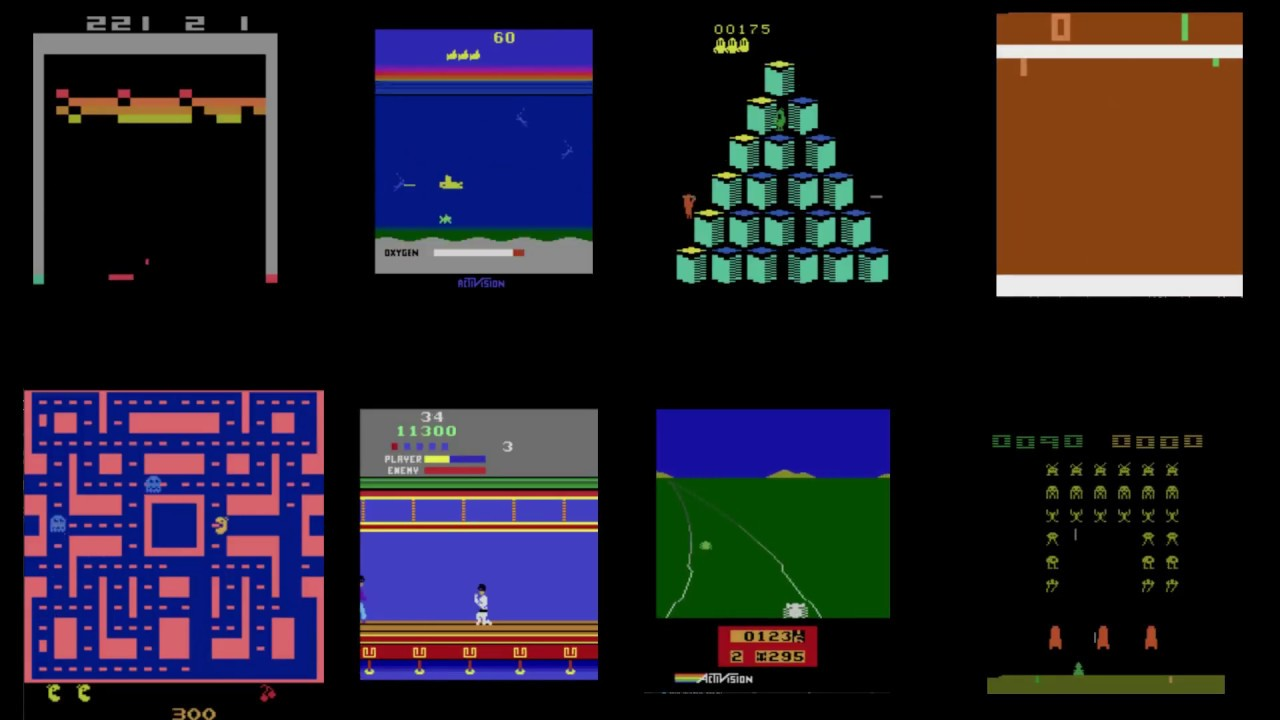
\includegraphics[width=10cm]{./Images/Chapter02/atari_games}
  \caption{A visual representation of some of the \texttt{Atari} games that are part of the Arcade Learning Environment (ALE) \cite{bellemare2013arcade}. From left to right \texttt{Breakout, Seaquest, Pong, MsPacman, Qbert, Kungfu-Master, Enduro} and \texttt{Space Invaders}. Most of these games will be of interest in chapters \ref{ch:dqv_family_of_algorithms} and \ref{ch:dqn_transfer}. Image courtesy of .}
  \label{fig:atari_games}
\end{figure}


\paragraph{Double Deep Q-Learning (DDQN)} \citet{van2016deep} showed that the DQN algorithm suffers from the same issue that also characterizes the Q-Learning algorithm: the overestimation bias of the $Q$ function. They show that DQN is prone to learn overestimated Q-values because the same values are used both for selecting an action ($\underset{a\in \mathcal{A}}{\max}$) and for evaluating it ($Q(s_{t+1},a;\theta^{-})$). This becomes clearer when re-writing DQN's TD-target presented in Eq. \ref{eq:dqn_td} as:
\begin{equation}
    y^{DQN}_{t} = r_{t} + \gamma \: Q(s_{t+1}, \underset{a\in \mathcal{A}}{\argmax}\: Q(s_{t+1}, a; \theta); \theta^{-}).
\end{equation}{}
As a result, DQN tends to approximate the expected maximum value of a state, instead of its maximum expected value. As presented in Sec. \ref{sec:td_learning}, in the tabular case this can be solved by keeping track of two separate $Q$ functions, and by randomly preferring one $Q$ function over the other when it comes to selecting which action to execute. DDQN generalizes this idea and untangles the action selection process from its evaluation by taking advantage of the previously introduced target network $\theta^{-}$. DDQN's target stays the same as in DQN with the main difference being that the selection of an action, given by the online Q-network $\theta$, and the evaluation of the resulting policy, given by $\theta^{-}$, can now result into smaller overestimations simply by symmetrically updating the two sets of weights ($\theta$ and $\theta^{-}$) which can easily be achieved by regularly switching their roles during training. While not always significantly impacting the performance of DQN (one can still act optimally even if some actions are associated to unrealistically high $Q(s,a)$ estimates), there are also cases for which the overestimation bias of the $Q$ function significantly slows down the training process and even prevents the DQN algorithm from improving its policy over time at all. We will come back to this issue in Chapter \ref{ch:dqv_family_of_algorithms}. 


\paragraph{Prioritized Experience Replay}
\paragraph{Dueling Networks}
\paragraph{Rainbow}


\section{Deep Reinforcement Learning Challenges}
non stationarity


\begin{remark}{Conclusion}

\end{remark}



 % ICCVTA paper

\cleardoublepage % Empty page before the start of the next part

%------------------------------------------------

\ctparttext{You can put some informational part preamble text here. Illo principalmente su nos. Non message \emph{occidental} angloromanic da. Debitas effortio simplificate sia se, auxiliar summarios da que, se avantiate publicationes via. Pan in terra summarios, capital interlingua se que. Al via multo esser specimen, campo responder que da. Le usate medical addresses pro, europa origine sanctificate nos se.} % Text on the Part 2 page describing the content in Part 2

\part{Transfer Learning for Deep Reinforcement Learning} % Second part of the thesis

%Chapter 7

\chapter{The Deep Quality-Value Learning Family of Algorithms} % Chapter title
\label{ch:dqv_family_of_algorithms} % For referencing the chapter elsewhere, use \autoref{ch:introduction} 


\begin{remark}{Contributions and Outline}
	In the second part of this thesis we have thoroughly studied the level of transferability of deep neural networks that get trained in a supervised learning fashion. From the results of our studies we concluded that significant benefits can come from using pre-trained models over networks that get trained from scratch, and that transfer learning can be a valuable machine learning paradigm for studying the generalization properties of neural networks. In this third, last part of this dissertation we will study whether adopting transfer learning strategies can be as useful in a Deep Reinforcement Learning (DRL) context, where convolutional neural networks get trained for solving optimal control problems. Before studying such transfer learning properties, however, we will start by contributing to the DRL literature by introducing a novel family of DRL algorithms. Therefore, this chapter does not study DRL algorithms from a transfer learning perspective yet, but rather introduces some novel techniques whose transfer learning properties will be researched in the next chapter.
	The structure of this chapter is the following: in Sec. \ref{sec:ijcnn_introduction} we remind the reader with some background information about the field of DRL and recall the mathematical notation that will be used throughout this chapter. In Sec. \ref{sec:dqv_family} we introduce the main algorithmic contributions of our research: a novel family of DRL algorithms the performance of which is thoroughly studied from different perspectives in Sec. \ref{sec:ijcnn_results}. The chapter ends with Sec. \ref{sec:ijcnn_additional_studies} and Sec. \ref{sec:ijcnn_discussion} where we provide a set of additional studies that characterize the performance of our newly introduced algorithms further, and critically discuss their properties. 
\vspace{5mm}

This chapter combines the work presented in the following publications: \citet{sabatelli2018deepqv}, \citet{sabatelli2019approximating}, and \citet{sabatelli2020deep}
\end{remark}

\section{Motivation}
\label{sec:ijcnn_introduction}

In Chapter \ref{ch:reinforcement_learning} we have seen that the aim of value-based Reinforcement Learning (RL) is to construct algorithms which learn value functions that are either able to estimate how good or bad it is for an agent to be in a particular state, or how good it is for an agent to perform a particular action in a given state. Such functions are respectively denoted as the state-value function $V(s)$, and the state-action value function $Q(s,a)$ \cite{sutton2018reinforcement}. We have then seen that in Deep Reinforcement Learning (DRL) the aim is to approximate these value functions with e.g., deep convolutional neural networks \cite{lecun2015deep}, as these kind of networks can serve as universal function approximators as well as powerful feature extractors. Classic model-free RL algorithms like Q-Learning \cite{watkins1992q}, Double Q-Learning \cite{hasselt2010double} and SARSA \cite{rummery1994line} have all led to the development of a ``deep'' version of themselves in which the original RL update rules are expressed as objective functions that can be minimized by gradient descent \cite{mnih2015human, van2016deep, zhao2016deep}. Despite their successful applications \cite{li2017deep}, however, the aforementioned algorithms only aim at approximating the $Q$ function, while completely ignoring the $V$ function, which is an approach that is prone to issues that go back to standard RL literature. As shown by \citet{van2016deep} the DQN algorithm \cite{mnih2015human} is known to overestimate the values of the $Q$ function and requires an additional target network to not diverge (which role, as shown by \citet{achiam2019towards}, is not yet fully understood). These overestimations can partially be corrected by the DDQN \cite{van2016deep} algorithm (see Sec. \ref{sec:deep_reinforcement_learning} of Chapter \ref{ch:reinforcement_learning}), which, despite yielding stability improvements, does not always prevent its $Q$ networks from diverging \cite{van2018deep_triad} and sometimes even underestimating the $Q$ function. Furthermore, DRL algorithms are also extremely slow to train. In what follows, we introduce a new family of DRL algorithms based on the key idea of simultaneously learning the $V$ function alongside the $Q$ function with two separate neural networks. Our main insight is that by jointly approximating the $V$ function and the $Q$ function, the task of learning one of these value functions can be sped up if the model that is responsible for learning it, can rely on what is being learned by the model responsible for learning the other value function. We show that this simple, yet effective idea yields faster, more robust and better model-free Deep Reinforcement Learning.


\section{A Novel Family of Deep Reinforcement Learning Algorithms}
\label{sec:dqv_family}

Just as much as DQN and DDQN are based on two tabular RL algorithms, so is the new family of algorithms presented in this chapter. More specifically we extend two RL algorithms which were first introduced by \citet{wiering2005qv} and then extended by \citet{wiering2009qv} to the use of deep neural networks that serve as function approximators. Training these algorithms robustly is done by taking advantage of some of the techniques which have been reviewed in Chapter \ref{ch:reinforcement_learning}.

\subsection{DQV-Learning}
Our first contribution is the Deep Quality-Value (DQV) Learning algorithm, a novel DRL algorithm which aims at jointly approximating the $V$ function alongside the $Q$ function in an \textcolor{RoyalBlue}{on-policy} learning setting. This algorithm is based on the QV($\lambda$) algorithm \cite{wiering2005qv}, a tabular RL algorithm which was reviewed in Chapter \ref{ch:reinforcement_learning} and that learns the $V$ function via the simplest form of TD-Learning \cite{sutton1988learning}. The estimates that are learned by this value function are then used to update the $Q$ function in a Q-Learning resembling way. Specifically, after a RL transition $\langle$ $s_{t}$, $a_{t}$, $r_{t}$, $s_{t+1}$ $\rangle$, QV$(\lambda)$ uses the TD$(\lambda)$ learning rule \cite{sutton1988learning} to update the $V$ function for all states: 
\begin{equation}
V(s):= V(s) + \alpha \big[ r_{t} + \gamma V(s_{t+1}) - V(s_t) \big] e_{t}(s),
\label{eq:qv_lambda_v_update}
\end{equation}
where $\alpha$ stands for the learning rate and $\gamma$ is the discount factor, while $e_t(s)$ are the elibility traces \cite{peng1994incremental, wiering1998speeding, geist2014off} that are necessary for keeping track if a particular state has occurred before a certain time-step or not. These are updated for all states as follows:  
\begin{equation} 
e_{t}(s) = \gamma \lambda e_{t-1}(s) + \eta_t(s),
\end{equation}
where $\eta_t(s)$ is an indicator function that returns a value of $1$ whether a particular state occurred at time $t$ and $0$ otherwise. Before updating the $V$ function, QV$(\lambda)$ updates the $Q$ function first, and does this via the following update rule:
\begin{equation}
Q(s_{t}, a_{t}):= Q(s_{t}, a_{t}) + \alpha \big[r_{t} + \gamma V(s_{t+1}) - Q(s_{t}, a_{t}) \big].
\label{eq:qv_lambda_q_update}
\end{equation}

We take inspiration from this specific learning dynamic and aim at learning an approximation of both the $V$ function, and the $Q$ function, with two neural networks that are respectively parametrized by $\Phi$ and $\theta$. To do so, we follow the same principles which have led to the development of the DQN algorithm. Therefore, starting from Eq. \ref{eq:qv_lambda_v_update}, and after removing $e_{t}(s)$ for simplicity, we get the following objective function which is used by DQV for learning the state-value function:
\begin{multline}
L(\Phi) = \mathds{E}_{\langle s_{t},a_{t},r_{t},s_{t+1}\rangle\sim U(D)} \bigg[\big(r_{t} + \gamma V(s_{t+1}; \Phi^{-}) - V(s_{t}; \Phi)\big)^{2}\bigg],
\label{eq:dqv_v_update}
\end{multline}
while the following loss is minimized for learning the $Q$ function when starting from Eq. \ref{eq:qv_lambda_q_update}:
\begin{multline}
    L(\theta) = \mathds{E}_{\langle s_{t},a_{t},r_{t},s_{t+1}\rangle\sim U(D)} \bigg[\big(r_{t} + \gamma V(s_{t+1}; \Phi^{-}) - Q(s_{t}, a_{t}; \theta)\big)^{2}\bigg],
\label{eq:dqv_q_update}
\end{multline}
where $D$ is the Experience-Replay memory buffer, used for uniformly sampling batches of RL trajectories $\langle s_{t},a_{t},r_{t},s_{t+1}\rangle$, and $\Phi^{-}$ is the target-network used for the construction of the TD-errors. Note that the role of this target network is different from its role within the DQN algorithm reviewed in Chapter \ref{ch:reinforcement_learning}. In DQV, this network corresponds to a copy of the network which approximates the state-value function and not the state-action value function. It is also worth noting that both networks learn from the same TD-target which comes in the following form:
\begin{equation}
y_{t}^{DQV} = r_{t} + \gamma V(s_{t+1}; \Phi^{-}). 
\end{equation}

\subsection{DQV-Learning with Multilayer Perceptrons}
We start by exploring whether this learning dynamic of jointly approximating two value functions simultaneously, and let the $Q$ function bootstrap from the TD-targets that are learned from the $V$ network, can yield successful results on a set of preliminary experiments. To do so, we use two classic control problems that are well known in the RL literature: \texttt{Acrobot} \cite{sutton1996generalization} and \texttt{Cartpole} \cite{barto1983neuronlike} with both environments being provided by the Open-AI Gym package \cite{brockman2016openai}. We approximate the $V$ function and the $Q$ function with a two hidden layer Multilayer Perceptron (MLP) that is activated by a ReLU non linearity ($f(x) = max (0,x)$) and compare the performance of DQV to the one of the DQN and the DDQN algorithms, which use the same MLP but for approximating the $Q$ function only. Given the simplicity of these two control problems we did not integrate DQV with the target network $\Phi^{-}$ yet. Our preliminary results reported in Fig. \ref{fig:mlp_dqv_results}, show the benefits that can come from training two separate networks with the update rules reported in Eq. \ref{eq:dqv_v_update} and Eq. \ref{eq:dqv_q_update}. We can in fact observe that on both control problems DQV-Learning outperforms DQN and DDQN, by converging significantly faster. 

\begin{figure}[ht!]
  \begin{tikzpicture}[scale = 0.65]
      \begin{axis}[
	name=ax1,
      	grid style={dashed,gray},
      	grid = both, 
      	tick style=black,
	title=Acrobot,
        xlabel=Episodes,
        ylabel=Reward,
      ]


      \addlegendentry{DQV}
      \addlegendentry{DQN}
      \addlegendentry{DDQN}
      
      \addplot [ultra thick, red, mark=.] table [y=DQV, x=episodes]
      {./Results/Chapter07/logs/acrobot_results.txt};
      \addplot [ultra thick, blue, mark=.] table [y=DQN, x=episodes]{./Results/Chapter07/logs/acrobot_results.txt};
      \addplot [ultra thick, green, mark=.] table [y=DDQN, x=episodes]{./Results/Chapter07/logs/acrobot_results.txt};
     
      \legend{}

      \end{axis}

      \begin{axis}[
	at={(ax1.south east)},
	xshift=2cm,
      	grid style={dashed,gray},
      	grid = both, 
      	tick style=black,
	title=Cartpole,
        xlabel=Episodes,
        ylabel= Reward,
	legend columns=3, 
        legend style={font=\Large, at={(-0.65,-0.3,-0.4)},anchor=north west,legend columns=3},
      ]

      \addlegendentry{DQV}
      \addlegendentry{DQN}
      \addlegendentry{DDQN}
 
      \addplot [ultra thick, red, mark=.] table [y=DQV, x=episodes]
      {./Results/Chapter07/logs/cartpole_results.txt};
      \addplot [ultra thick, blue, mark=.] table [y=DQN, x=episodes]{./Results/Chapter07/logs/cartpole_results.txt};
      \addplot [ultra thick, green, mark=.] table [y=DDQN, x=episodes]{./Results/Chapter07/logs/cartpole_results.txt};
 
      \end{axis}
	\end{tikzpicture}
	\caption{}
	\label{fig:mlp_dqv_results} 
\end{figure}




\subsection{DQV-Max Learning}
Based on the successful results presented in Fig. \ref{fig:mlp_dqv_results} that highlight the potential benefits that could come from jointly approximating two value functions over one, we now introduce the Deep Quality-Value-Max (DQV-Max) algorithm, a novel DRL algorithm which builds on top of some of the ideas that characterize DQV. Similarly as done for DQV, we still aim at jointly learning an approximation of the $V$ function and the $Q$ function, but in this case, the goal is to do this with an \textcolor{RoyalBlue}{off-policy} learning scheme. To construct this algorithm we take inspiration from the QV-Max RL algorithm introduced by \citet{wiering2009qv}. The key component of QV-Max is the use of the $\underset{a\in \mathcal{A}}{\max}\: Q(s_{t+1}, a)$ operator, which makes RL algorithms learn off-policy. We use this operator when approximating the $V$ function and for computing TD-errors which correspond to the ones that are also used by the DQN algorithm. However, within DQV-Max, these TD-errors are used by the state-value network and not by the state-action value network. This results in the following loss which is used for learning the $V$ function:
\begin{multline}
L(\Phi) = \mathds{E}_{\langle s_{t},a_{t},r_{t},s_{t+1}\rangle\sim U(D)} \bigg[\big(r_{t} + \gamma \: \underset{a\in \mathcal{A}}{\max}\: Q(s_{t+1}, a; \theta^{-}) - V(s_{t}; \Phi)\big)^{2}\bigg].
\label{eq:dqv_max_v}
\end{multline}
In this case the target network $\theta^{-}$ corresponds to the same target network that is also used by DQN. The TD-error $r_{t} + \gamma \: \underset{a\in \mathcal{A}}{\max}\: Q(s_{t+1}, a; \theta^{-})$ is however only used for learning the $V$ function. When it comes to the $Q$ function we use the same update rule that is presented in Eq. \ref{eq:dqv_q_update} with the only difference being that in this case no $\Phi^{-}$ target network is used. Despite requiring the computation of two different targets for learning, we noticed that DQV-Max did not benefit from using two distinct target networks, therefore its loss function for approximating the $Q$ function is simply:
\begin{multline}
    L(\theta) = \mathds{E}_{\langle s_{t},a_{t},r_{t},s_{t+1}\rangle\sim U(D)} \bigg[\big(r_{t} + \gamma V(s_{t+1}; \Phi) - Q(s_{t}, a_{t}; \theta)\big)^{2}\bigg].
    \label{eq:dqv_max_q}
\end{multline}

The pseudocode of both DQV and DQV-Max is presented at the end of this thesis in Algorithm \ref{alg: dqv_algorithms} which can be found in Appendix \ref{ch:appendixDQV}. The pseudocode is an adaptation of a standard DRL training loop which corresponds to what is usually presented within the literature \cite{mnih2015human}. We just make explicit use of the hyperparameters \texttt{total\_a} and \texttt{c} which ensure that enough actions have been performed by the agent before updating the weights of the target network. We also ensure via the hyperparameter \texttt{total\_e}, that enough episodes are stored within the memory buffer (which has capacity $\mathcal{N}$) before starting to optimize the neural networks. 



\section{Results}
\label{sec:ijcnn_results}

\subsection{Global Evaluation}
\label{sec:global_evaluation}

We evaluate the performance of DQV and DQV-Max on a subset of 15 games coming from the popular \texttt{Atari-2600} benchmark \cite{bellemare2013arcade}. Our newly introduced algorithms are compared against DQN and DDQN. To keep all the comparisons as fair as possible we follow the same experimental setup and evaluation protocol which was used in \cite{mnih2015human} and \cite{van2016deep}. The only difference between DQV and DQV-Max, and DQN and DDQN is the exploration schedule which is used. Differently from the latter two algorithms, which use an epsilon-greedy strategy which has an $\epsilon$ starting value of 1.0, DQV and DQV-Max's exploration policy starts with an initial $\epsilon$ value of 0.5. All other hyperparameters, ranging from the size of the Experience-Replay memory buffer to the architectures of the neural networks, are kept the same among all algorithms. We refer the reader to the original DQN paper \cite{mnih2015human} for an in-depth overview of all these hyperparameters. The performance of the algorithms is tested based on the popular \texttt{no-op action} evaluation regime. At the end of the training, the learned policies are tested over a series of episodes for a total amount of 5 minutes of emulator time. All testing episodes start by executing a set of partially random actions to test the level of generalization of the learned policies. We present our results in Table \ref{tab:ch07_results} where the best performing algorithm is reported in a green cell while the second-best performing algorithm is reported in a yellow cell. As is common within the DRL literature, the table also reports the scores which would be obtained by an expert human player and by a random policy. When the scores over games are equivalent, we report in the green and yellow cells the fastest and second fastest algorithm with respect to its convergence time (determined by a visual inspection of the learning curves). 

We can start by observing that DQV and DQV-Max successfully master all the environments on which they have been tested, with the only exception being the \texttt{Montezuma's Revenge} game. It is well-known that this game requires more sophisticated exploration strategies than the epsilon-greedy one \cite{fortunato2017noisy}, and was also not mastered by DQN and DDQN when these algorithms were introduced. We can also observe that there is no algorithm which performs best on all the tested environments even though, as highlighted by the green and yellow cells, the algorithms of the DQV-family seem to generally perform better than DQN and DDQN, with DQV-Max being the overall best performing algorithm in our set of experiments. When either DQV or DQV-Max are not the best performing algorithm (see for example the \texttt{Boxing} and \texttt{Crazy Climber} environments), we can still observe that our algorithms managed to converge to a policy which is not significantly worst than the one learned by DQN and DDQN.
There is however one exception being the \texttt{Road Runner} environment. In fact, in this game, DDQN significantly outperforms DQV and DQV-Max. It is also worth noting the results on the \texttt{Bank Heist} and \texttt{Enduro} environments. Both DQN and DDQN failed to achieve super-human performance on these games, while DQV and DQV-Max successfully managed to obtain a significantly higher score than the one obtained by a professional human player. On the \texttt{Bank Heist} environment DQV and DQV-Max obtain $\approx 400$ points more than an expert human player, while on the \texttt{Enduro} environment their performance is almost three times better than the one obtained by DQN and DDQN.

\begin{table*}[ht]
\caption{The results obtained by DQV and DQV-Max on a subset of 15 \texttt{Atari} games, compared with those obtained by DQN and DDQN (reproduced from their corresponding publications). We can see that our newly introduced algorithms have a comparable, and often even better performance than DQN and DDQN. As highlighted by the green cells the overall best performing algorithm in our set of experiments is DQV-Max while the second-best performing algorithm is DQV (as reported by the yellow cells). Specific attention should be given to the games \texttt{BankHeist} and \texttt{Enduro} where DQV and DQV-Max are the only algorithms which can master the game with a final super-human performance.}
\centering
\resizebox{\columnwidth}{!}{%
\begin{tabular}{l|r|r|r|r|r|r}
\hline 
Environment & Random & Human & DQN \cite{mnih2015human} & DDQN \cite{van2016deep} & DQV & DQV-Max\\
\hline \hline
\texttt{Asteroids} &719.10 &13156.70 &\cellcolor{yellow!25}1629.33 &930.60 &1445.40 & \cellcolor{green!25}1846.08\\
\texttt{Bank Heist} &14.20 & 734.40 & 429.67 & 728.30 & \cellcolor{green!25}1236.50 & \cellcolor{yellow!25}1118.28 \\
\texttt{Boxing} &0.10 & 4.30 & 71.83 & \cellcolor{green!25}81.70 & 78.66 & \cellcolor{yellow!25}{80.15} \\
\texttt{Crazy Climber} &10780.50 & 35410.50 & \cellcolor{green!25}114103.33 & 101874.00 & \cellcolor{yellow!25}108600.00 & 1000131.00\\
\texttt{Enduro} &0.00 & 309.60 & 301.77 & 319.50 & \cellcolor{yellow!25}829.33 & \cellcolor{green!25}875.64 \\
\texttt{Fishing Derby} &-91.70 & 5.50 & -0.80 & \cellcolor{yellow!25}20.30 & 1.12 & \cellcolor{green!25}20.42  \\
\texttt{Frostbite} &65.20 & 4334.70 & \cellcolor{green!25}328.33 & 241.50 & 271.86 & \cellcolor{yellow!25}281.36 \\
\texttt{Gopher} &257.60 & 2321.00 &\cellcolor{green!25}{8520.00} &8215.40 &\cellcolor{yellow!25}{8230.30} &7940.00 \\
\texttt{Ice Hockey} &-11.20 & 0.90 & \cellcolor{yellow!25}-1.60 & -2.40 & -1.88 & \cellcolor{green!25}-1.12\\
\texttt{James Bond} &29.00 & 406.70 & \cellcolor{green!25}{576.67} & 438.00 & 372.41 & \cellcolor{yellow!25}{440.80} \\
\texttt{Montezuma's Revenge} &0.00 & 4366.70 & 0.00 & 0.00 & 0.00 & 0.00\\
\texttt{Ms.Pacman} &307.30 & 15693.40 & 2311.00 & 3210.00 & \cellcolor{green!25}3590.00 & \cellcolor{yellow!25}3390.00\\
\texttt{Pong} &-20.70 &9.30 & 18.90 & 21.00 & \cellcolor{yellow!25}21.00 & \cellcolor{green!25}21.00\\
\texttt{Road Runner} &11.50 &7845.00 &18256.67  &\cellcolor{green!25}48377.00  &\cellcolor{yellow!25}39290.00  & 20700.00\\
\texttt{Zaxxon} &32.50 &9173.30 &4976.67  &\cellcolor{yellow!25}10182.00  &\cellcolor{green!25}10950.00  & 8487.00\\

\end{tabular}%
}
\label{tab:ch07_results}
\end{table*}



\subsection{Convergence Time}
\label{sec:convergence_time}

While DRL algorithms have certainly obtained impressive results on the \texttt{Atari-2600} benchmark, it is also true that the amount of training time which is required by these algorithms can be very long. Over the years, several techniques reviewed in Sec. \ref{sec:deep_reinforcement_learning} of Chapter \ref{ch:reinforcement_learning}, ranging from Prioritized Experience Replay (PER) \cite{wang2016dueling} to the Rainbow extensions introduced by \citet{hessel2018rainbow}, have been proposed to reduce the training time of DRL algorithms. It is therefore natural to investigate whether jointly approximating the $V$ function alongside the $Q$ function can lead to significant benefits in this behalf. Unlike the $Q$ function
    \begin{align*}
	     Q^{\pi}(s,a)=\mathds{E}\bigg[\sum_{k=0}^{\infty}\gamma^{k}r_{t+k} \bigg| s_t = s, a_t=a, \pi\bigg],
    \end{align*}
recall that the state-value function
  \begin{align*}
	    V^{\pi}(s)=\mathds{E}\bigg[\sum_{k=0}^{\infty}\gamma^{k}r_{t+k}\bigg| s_t = s, \pi \bigg],
    \end{align*}
 is not conditioned on the set of possible actions that the agent may take, and therefore requires fewer parameters to converge. Since DQV and DQV-Max use the estimates of the $V$ network to train the $Q$ function, it is possible that the $Q$ function could directly benefit from these estimates and as a result converge faster than when regressed towards itself (as happens in DQN).

We use two self-implemented versions of DQN and DDQN for comparing the convergence time that is required during training by all the tested algorithms on three increasingly complex \texttt{Atari} games: \texttt{Boxing, Pong} and \texttt{Enduro}. Our results, reported in Fig. \ref{fig:ch07_convergence_results}, show that DQV and DQV-Max converge significantly faster than DQN and DDQN, therefore confirming the preliminary results which we reported in Fig. \ref{fig:mlp_dqv_results}, and highlighting once again the benefits of jointly approximating two value functions instead of one when it comes to the overall convergence time that is required by the algorithms. Even though, as presented in Table \ref{tab:ch07_results}, DQV and DQV-Max do not always significantly outperform DQN and DDQN in terms of the final cumulative reward which is obtained, it is worth noting that these algorithms require significantly less training episodes to converge on all tested games. This benefit makes our two novel algorithms faster alternatives within model-free DRL.

\begin{figure}[ht!]
  \begin{tikzpicture}[scale = 0.65]
      \begin{axis}[
	name=ax1,
      	grid style={dashed,gray},
      	grid = both, 
      	tick style=black,
	title=Boxing,
        xlabel=Episodes,
        ylabel=Reward,
      ]


      \addlegendentry{DQV} 
      \addlegendentry{DQV-Max}  
      \addlegendentry{DQN}
      \addlegendentry{DDQN}
      
      \addplot [ultra thick, red, mark=.] table [y=DQV, x=episodes]
      {./Results/Chapter07/logs/boxing_results.txt};
       \addplot [ultra thick, yellow, mark=.] table [y=DQV-Max, x=episodes]
      {./Results/Chapter07/logs/boxing_results.txt};
      \addplot [ultra thick, blue, mark=.] table [y=DQN, x=episodes]{./Results/Chapter07/logs/boxing_results.txt};
      \addplot [ultra thick, green, mark=.] table [y=DDQN, x=episodes]{./Results/Chapter07/logs/boxing_results.txt};
     
      \legend{}

      \end{axis}

      \begin{axis}[
      	at={(ax1.south east)},
	xshift=2cm,
	grid style={dashed,gray},
      	grid = both, 
      	tick style=black,
	title=Enduro,
        xlabel=Episodes,
        ylabel=Reward,
      ]


      \addlegendentry{DQV} 
      \addlegendentry{DQV-Max}  
      \addlegendentry{DQN}
      \addlegendentry{DDQN}
      
      \addplot [ultra thick, red, mark=.] table [y=DQV, x=episodes]
      {./Results/Chapter07/logs/enduro_results.txt};
       \addplot [ultra thick, yellow, mark=.] table [y=DQV-Max, x=episodes]
      {./Results/Chapter07/logs/enduro_results.txt};
      \addplot [ultra thick, blue, mark=.] table [y=DQN, x=episodes]{./Results/Chapter07/logs/enduro_results.txt};
      \addplot [ultra thick, green, mark=.] table [y=DDQN, x=episodes]{./Results/Chapter07/logs/enduro_results.txt};
     
      \legend{}

      \end{axis}


      \begin{axis}[
	at={(ax1.south east)},
	xshift=-2cm,
      	yshift=-8cm,
	grid style={dashed,gray},
      	grid = both, 
      	tick style=black,
	title=Pong,
        xlabel=Episodes,
        ylabel= Reward,
	legend columns=4, 
        legend style={font=\Large, at={(-0.3,-0.3,-0.4)},anchor=north west,legend columns=3},
      ]


	\addlegendentry{DQV} 
	\addlegendentry{DQV-Max}  
	\addlegendentry{DQN}
	\addlegendentry{DDQN}

      \addplot [ultra thick, red, mark=.] table [y=DQV, x=episodes]
      {./Results/Chapter07/logs/pong_results.txt};
      \addplot [ultra thick, yellow, mark=.] table [y=DQV-Max, x=episodes]
      {./Results/Chapter07/logs/pong_results.txt};
      
      \addplot [ultra thick, blue, mark=.] table [y=DQN, x=episodes]{./Results/Chapter07/logs/pong_results.txt};
      \addplot [ultra thick, green, mark=.] table [y=DDQN, x=episodes]{./Results/Chapter07/logs/pong_results.txt};
 
      \end{axis}
	\end{tikzpicture}
	\caption{Learning curves obtained during training on three different \texttt{Atari} games by DQV and DQV-Max, and DQN and DDQN. We can observe that on these games both DQV and DQV-Max converge significantly faster than DQN and DDQN and that they obtain higher cumulative rewards on the \texttt{Enduro} environment.}
	\label{fig:ch07_convergence_results} 
\end{figure}



\subsection{Quality of the Learned Value Functions}
\label{sec:quality_of_value_functions}

It is well-known that the combination of RL algorithms with function approximators can yield DRL algorithms that diverge. The popular Q-Learning algorithm is known to result in unstable learning both if linear \cite{tsitsiklis1997analysis} and non-linear functions are used when approximating the $Q$ function \cite{van2018deep_triad}. As seen at the end of Chapter \ref{ch:reinforcement_learning}, this divergence according to \citet{sutton2018reinforcement} is caused by the interplay of three elements that are known as the \textit{`Deadly Triad'} of DRL. The elements of this triad are:
\begin{itemize}
    \item \textit{a function approximator}: which is used for learning an approximation of a value function that could not be learned in the tabular RL setting due to a too large state-action space.
    \item \textit{bootstrapping}: when the algorithms use a future estimated value for learning the same kind of estimate.
    \item \textit{off-policy learning}: when a future estimated value is different from the one which would be computed by the policy the agent is following.
\end{itemize}{}

\citet{van2018deep_triad} have shown that the \textit{`Deadly Triad'} is responsible for enhancing one of the most popular biases that characterize the Q-Learning algorithm: the overestimation bias of the $Q$ function \cite{hasselt2010double}. It is therefore natural to study how DQV and DQV-Max relate to the \textit{`Deadly Triad'} of DRL, and to investigate up to what extent these algorithms suffer from the overestimation bias of the $Q$ function. To do this we monitor the estimates that are given by the network that is responsible for approximating the $Q$ function. More specifically, at training time, we compute the averaged $\underset{a \in \cal A}{\max}\:Q(s_{t+1}, a)$ over a set ($n$) of full evaluation episodes as defined by 
\begin{equation}
\frac{1}{n}\sum_{t=1}^{n}\underset{a \in \cal A}{\max}\:Q(s_{t+1}, a;\theta).
\end{equation}
As suggested by \citet{van2016deep} these estimates can then be compared to the averaged discounted return of all visited states that comes from an agent that has already concluded training. By analyzing whether the $Q$ values which are estimated while training differ from the ones which should be predicted by the end of it, it is possible to quantitatively characterize the level of divergence of DRL algorithms. We report our results in Figs. \ref{fig:overestimation_bias_results_dqn}, \ref{fig:overestimation_bias_results_ddqn}, \ref{fig:overestimation_bias_results_dqv} and \ref{fig:overestimation_bias_results_dqv_max} where the black full lines correspond to the value estimates that come from each algorithm at training time, while the coloured lines correspond to the actual averaged discounted return that is given by an already trained agent.


We can start by observing that the values denoting the averaged discounted return obtained by each algorithm differ among agents. This is especially the case when it comes to the \texttt{Enduro} environment, and is a result which is in line with what has been presented in Table \ref{tab:results}: DQV and DQV-Max lead to better final policies than DQN and DDQN. Furthermore, when we compare these baseline values to the value estimates that are obtained during training, we can observe that the ones obtained by the DQN algorithm significantly diverge from the ones which should be predicted by the end of training. This behavior is known to be caused by the overestimation bias of the $Q$ function which can be corrected by the DDQN algorithm. By analyzing the value estimates of DQV and DQV-Max we can observe that both algorithms produce value estimates which are more similar to the ones computed by DDQN than to the ones given by DQN. This is especially the case for DQV (Fig. \ref{fig:overestimation_bias_results_dqv}). In fact, its value estimates nicely correspond to the averaged discounted return baseline, both on the \texttt{Pong} environment and on the \texttt{Enduro} environment. The estimates coming from DQV-Max, however, seem to diverge more when compared to DQV and DDQN's ones. This is clearer on the \texttt{Enduro} environment, where the algorithm does show some divergence (right plot of Fig. \ref{fig:overestimation_bias_results_dqv_max}). However, we can also observe that this divergence is less strong when compared to DQN's one. The value estimates of the latter algorithm keep growing over time, while DQV-Max's ones get bounded while training progresses (see the two right plots of Fig. \ref{fig:overestimation_bias_results_dqn} and Fig. \ref{fig:overestimation_bias_results_dqv_max}). This results in smaller estimated $Q$ values. We believe that there are mainly two reasons why our algorithms suffer less from the overestimation bias of the $Q$ function. When it comes to DQV, we believe that this algorithm suffers less from this bias since it is an on-policy learning algorithm. Such algorithms are trained on exploration actions with lower $Q$ values. Because of its \textit{on-policy} learning scheme, DQV also does not present one element of the \textcolor{RoyalBlue}{`Deadly Triad'}, which might help reducing divergence. When it comes to DQV-Max, we believe that the reason why this algorithm does not diverge as much as DQN can be found in the way it approximates the $Q$ function. One key component of the \textit{`Deadly Triad'}, is that divergence occurs if the $Q$ function is learned by regressing towards itself. As given by Eq. \ref{eq:dqv_max_q} we can see that this does not hold for DQV-Max, since the $Q$ function bootstraps with respect to estimates that come from the $V$ network. We believe that this specific learning dynamic, which also holds for the DQV algorithm, makes our algorithms less prone to estimate large $Q$ values.

% add overestimation bias results
\begin{figure}[ht!]
  \begin{tikzpicture}[scale = 0.65]
      \begin{axis}[
	name=ax1,
      	grid style={dashed,gray},
      	grid = both, 
      	tick style=black,
	title=Pong,
        xlabel=Training Steps,
        ylabel=Value Estimates,
      ]


      \addlegendentry{DQN-True Value}
      \addlegendentry{DQN-Estimated Value}
      
      \addplot [ultra thick, black, mark=.] table [y=true_return_DQN, x=training_steps]
      {./Results/Chapter07/logs/overestimation_pong.txt};
      \addplot [ultra thick, blue, mark=.] table [y=estimate_DQN, x=training_steps]{./Results/Chapter07/logs/overestimation_pong.txt};
     
      \legend{}

      \end{axis}

      \begin{axis}[
	at={(ax1.south east)},
	xshift=2cm,
      	grid style={dashed,gray},
      	grid = both, 
      	tick style=black,
	title=Enduro,
        xlabel=Training Steps,
        ylabel= Value Estimates,
	legend columns=3, 
        legend style={font=\Large, at={(-0.85,-0.3,-0.4)},anchor=north west,legend columns=3},
      ]

      \addlegendentry{DQN-True Value}
      \addlegendentry{DQN-Estimated Value}

      \addplot [ultra thick, black, mark=.] table [y=true_return_DQN, x=training_steps]
      {./Results/Chapter07/logs/overestimation_enduro.txt};
      \addplot [ultra thick, blue, mark=.] table [y=estimate_DQN, x=training_steps]{./Results/Chapter07/logs/overestimation_enduro.txt};
 
      \end{axis}
	\end{tikzpicture}
	\caption{}
	\label{fig:overestimation_bias_results} 
\end{figure}


\begin{figure}[ht!]
  \begin{tikzpicture}[scale = 0.65]
      \begin{axis}[
	name=ax1,
      	grid style={dashed,gray},
      	grid = both, 
      	tick style=black,
	title=Pong,
        xlabel=Training Steps,
        ylabel=Value Estimates,
      ]


      \addlegendentry{DDQN-True Value}
      \addlegendentry{DDQN-Estimated Value}
      
      \addplot [ultra thick, black, mark=.] table [y=true_return_DDQN, x=training_steps]
      {./Results/Chapter07/logs/overestimation_pong.txt};
      \addplot [ultra thick, green, mark=.] table [y=estimate_DDQN, x=training_steps]{./Results/Chapter07/logs/overestimation_pong.txt};
     
      \legend{}

      \end{axis}

      \begin{axis}[
	at={(ax1.south east)},
	xshift=2cm,
      	grid style={dashed,gray},
      	grid = both, 
      	tick style=black,
	title=Enduro,
        xlabel=Training Steps,
        ylabel= Value Estimates,
	legend columns=3, 
        legend style={font=\Large, at={(-0.85,-0.3,-0.4)},anchor=north west,legend columns=3},
      ]

      \addlegendentry{DDQN-True Value}
      \addlegendentry{DDQN-Estimated Value}
      

      \addplot [ultra thick, black, mark=.] table [y=true_return_DDQN, x=training_steps]
      {./Results/Chapter07/logs/overestimation_enduro.txt};
      \addplot [ultra thick, green, mark=.] table [y=estimate_DDQN, x=training_steps]{./Results/Chapter07/logs/overestimation_enduro.txt};
 
      \end{axis}
	\end{tikzpicture}
	\caption{Results investigating the extent to which the DDQN algorithm suffers from the overestimation bias of the $Q$ function. We can observe that compared to the analysis presented in Fig. \ref{fig:overestimation_bias_results_dqn}, the DDQN algorithm prevents its Q-Network from diverging since on both \texttt{Atari} environments the $\underset{a \in \cal A}{\max}\:Q(s_{t+1}, a)$ estimates do not diverge from the observed real return of a trained agent. These results replicate the findings reported by \citet{van2018deep_triad}.}
	\label{fig:overestimation_bias_results_ddqn} 
\end{figure}


\begin{figure}[ht!]
  \begin{tikzpicture}[scale = 0.65]
      \begin{axis}[
	name=ax1,
      	grid style={dashed,gray},
      	grid = both, 
      	tick style=black,
	title=Pong,
        xlabel=Training Steps,
        ylabel=Value Estimates,
      ]


      \addlegendentry{DQV-True Value}
      \addlegendentry{DQV-Estimated Value}
      
      \addplot [ultra thick, black, mark=.] table [y=true_return_DQV, x=training_steps]
      {./Results/Chapter07/logs/overestimation_pong.txt};
      \addplot [ultra thick, red, mark=.] table [y=estimate_DQV, x=training_steps]{./Results/Chapter07/logs/overestimation_pong.txt};
     
      \legend{}

      \end{axis}

      \begin{axis}[
	at={(ax1.south east)},
	xshift=2cm,
      	grid style={dashed,gray},
      	grid = both, 
      	tick style=black,
	title=Enduro,
        xlabel=Training Steps,
        ylabel= Value Estimates,
	legend columns=3, 
        legend style={font=\Large, at={(-0.85,-0.3,-0.4)},anchor=north west,legend columns=3},
      ]

      \addlegendentry{DQV-True Value}
      \addlegendentry{DQV-Estimated Value}

      \addplot [ultra thick, black, mark=.] table [y=true_return_DQV, x=training_steps]
      {./Results/Chapter07/logs/overestimation_enduro.txt};
      \addplot [ultra thick, red, mark=.] table [y=estimate_DQV, x=training_steps]{./Results/Chapter07/logs/overestimation_enduro.txt};
 
      \end{axis}
	\end{tikzpicture}
	\caption{}
	\label{fig:overestimation_bias_results_ddqn} 
\end{figure}


\begin{figure}[ht!]
  \begin{tikzpicture}[scale = 0.65]
      \begin{axis}[
	name=ax1,
      	grid style={dashed,gray},
      	grid = both, 
      	tick style=black,
	title=Pong,
        xlabel=Training Steps,
        ylabel=Value Estimates,
      ]


      \addlegendentry{DQV-Max-True Value}
      \addlegendentry{DQV-Max-Estimated Value}
      
      \addplot [ultra thick, black, mark=.] table [y=true_return_DQV-Max, x=training_steps]
      {./Results/Chapter07/logs/overestimation_pong.txt};
      \addplot [ultra thick, yellow, mark=.] table [y=estimate_DQV-Max, x=training_steps]{./Results/Chapter07/logs/overestimation_pong.txt};
     
      \legend{}

      \end{axis}

      \begin{axis}[
	at={(ax1.south east)},
	xshift=2cm,
      	grid style={dashed,gray},
      	grid = both, 
      	tick style=black,
	title=Enduro,
        xlabel=Training Steps,
        ylabel= Value Estimates,
	legend columns=3, 
        legend style={font=\Large, at={(-1,-0.3,-0.4)},anchor=north west,legend columns=3},
      ]

      \addlegendentry{DQV-Max-True Value}
      \addlegendentry{DQV-Max-Estimated Value}

      \addplot [ultra thick, black, mark=.] table [y=true_return_DQV-Max, x=training_steps]
      {./Results/Chapter07/logs/overestimation_enduro.txt};
      \addplot [ultra thick, yellow, mark=.] table [y=estimate_DQV-Max, x=training_steps]{./Results/Chapter07/logs/overestimation_enduro.txt};
 
      \end{axis}
	\end{tikzpicture}
	\caption{Results investigating the extent to which the DQV-Max algorithm suffers from the overestimation bias of the $Q$ function. We can observe that on the \texttt{Pong} environment the value estimates of the algorithm are comparable to the ones of DDQN and DQV, therefore showing the DQV-Max also diverges significantly less than DQN. On the \texttt{Enduro} environment we can observe that the algorithm does diverge, although, differently from what is reported in Fig. \ref{fig:overestimation_bias_results_dqn}, the $\underset{a \in \cal A}{\max}\:Q(s_{t+1}, a)$ estimates seem to converge towards an upper bound ($\approx 15$). Similarly to what is reported in Fig.\ref{fig:overestimation_bias_results_dqv} we can again observe that the real return obtained by a trained agent is higher compared to the one obtain by DQN, DDQN and DQV, therefore confirming the results presented in Table \ref{tab:ch07_results} which see the DQV-Max algorithm as the best performing algorithm on the \texttt{Enduro} game.}
	\label{fig:overestimation_bias_results_dqv_max} 
\end{figure}




\section{Additional Studies}
\label{sec:ijcnn_additional_studies}

As introduced in Sec. \ref{sec:dqv_family} DQV and DQV-Max use two separate neural networks for approximating the $Q$ function and the $V$ function. To verify whether two different architectures are needed for making both algorithms perform well, we have experimented with a series of variants of the DQV-Learning algorithm. The aim of these experiments is that of reducing the number of trainable parameters that are required by the original version of DQV, and investigate whether its performance could get harmed when reducing the capacity of the algorithm. The studied DQV's extensions are the following:

\begin{enumerate}
    \item \textit{Hard-DQV}: a version of DQV which uses one single common neural network for approximating both the $Q$ and the $V$ functions. An additional output node (see Fig. \ref{fig:hard_dqv} for an impression of the architecture), needed for estimating the value of a state, is added next to the output nodes which estimate the different $Q$ values (one per action). The parameters of this algorithm are therefore `hardly-shared' among the agent, and provide the benefit of halving the total amount of trainable parameters of DQV. The different outputs of the network get then alternatively optimized according to Eq. \ref{eq:dqv_v_update} and \ref{eq:dqv_q_update}.

    \item \textit{Dueling-DQV}: a slightly more complicated version of Hard-DQV which adds one specific hidden layer before the output nodes that estimate the $Q$ and $V$ functions. In this case, the outputs of the neural network which learn one of the two value functions, partly benefit from some specific weights that are not shared within the neural network. This approach is similar to the one used by the `Dueling-Architecture' presented by \citet{wang2016dueling}, therefore the name Dueling-DQV. While it is well established that three convolutional layers are needed \cite{mnih2015human, van2016deep} for learning the $Q$ function, the same might not be true when it comes to learning the $V$ function. We thus report experiments with three different versions of Dueling-DQV: Dueling-1st, Dueling-2nd, and Dueling-3rd. The difference between these methods is simply the location of the hidden layer which precedes the output that learns the $V$ function. It can be positioned after the first convolutional layer, the second or the third one (see Fig. \ref{fig:dueling_dqv}). Training this architecture is done as for Hard-DQV.

    \item \textit{Tiny-DQV}: the neural architectures used by DQV and DQV-Max that approximate the $V$ function and the $Q$ function follow the one which was initially introduced by the DQN algorithm \cite{mnih2015human}. This corresponds to a three-hidden layer convolutional neural network which is followed by a fully connected layer of 512 hidden units. The first convolutional layer has 32 channels while the last two layers have 64 channels. In Tiny-DQV we reduce the number of trainable parameters of DQV by reducing the number of channels at each convolution operation. Tiny-DQV only uses 8 channels after the first convolutional layer and 16 at the second and third convolutional layers. Furthermore, the size of the final fully connected layer is reduced to only 128 hidden units. The choice of this architecture is motivated by the work presented in \cite{van2018deep_triad} which studies the role of the capacity of the DDQN algorithm. Unlike the Hard-DQV and Dueling-DQV extensions, the parameters of Tiny-DQV are not shared at all among the networks that are responsible for approximating the $V$ function and the $Q$ function.
\end{enumerate}

\begin{figure}[ht!]
  \makebox[\textwidth][c]{%
  \subfloat[]{\scalebox{0.25}{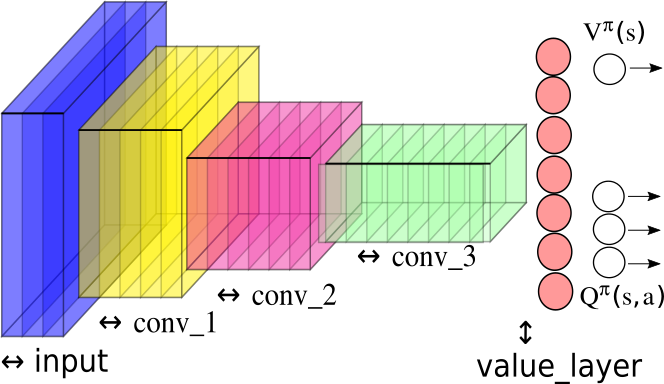
\includegraphics{./Images/Chapter07/DuelingDQV_shared.png}} \label{fig:hard_dqv}}
  \quad
  \subfloat[]{\scalebox{0.25}{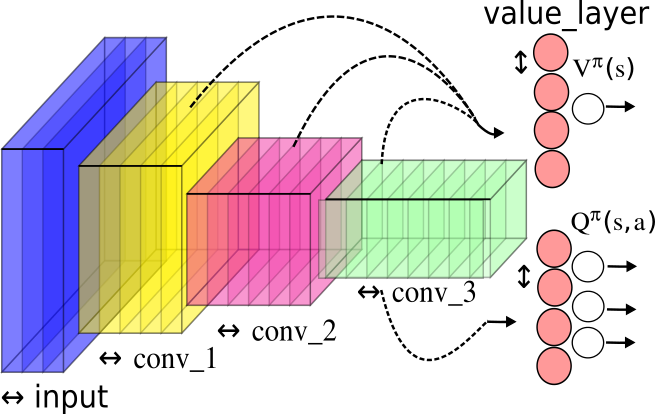
\includegraphics{./Images/Chapter07/dueling_DQV.png}} \label{fig:dueling_dqv}}
  }
\caption{Two representations of convolutional neural networks which jointly approximate the $V$ function and the $Q$ function with the aim of reducing DQV's learning parameters. On the left, an architecture which simply adds one output node to the network next to the output nodes which estimate the $Q$ function. On the right an architecture in which a specific hidden layer precedes the output that is necessary for computing each value function. When it comes to the $V$ function we experiment with different locations of such hidden layer, which is positioned after each possible convolution block.}
\end{figure}

The results obtained by these alternative versions of DQV are presented in Figs. \ref{fig:hard_dqv_results}, \ref{fig:duelling_dqv_results} and \ref{fig:tiny_dqv_results} where we report the learning curves obtained by the tested algorithms on six different \texttt{Atari} games. Each DQV extension is directly compared to the original DQV algorithm. We can observe that all the extensions of DQV, which aim at reducing the number of trainable parameters of the algorithm, fail in performing as well as the original DQV algorithm. Starting from Fig. \ref{fig:hard_dqv_results} we can observe that \textit{Hard-DQV} does not only yield significantly lower rewards (see the results obtained on \texttt{Boxing}) but also presents more unstable training (as highlighted by the results obtained on the \texttt{Pong} environment). Lower rewards and unstable training also characterize the \textit{Tiny-DQV} algorithm (see results on \texttt{Bank Heist} and \texttt{Crazy Climber} reported in Fig.\ref{fig:tiny_dqv_results}). Overall the most promising extensions of DQV are its \textit{Dueling} counterparts, we have observed in particular that the best performing architecture over most of our experiments was the \textit{Dueling-DQV-3rd} one. As can be seen by the results reported in Fig. \ref{fig:duelling_dqv_results} on the \texttt{Pong} environment we can observe that \textit{Dueling-DQV-3rd} has a comparable performance to DQV, even though it converges slower. Unfortunately, \textit{Dueling-DQV-3rd} still shows some limitations, in particular when tested on more complicated environments such as \texttt{Enduro}, we can observe that it under-performs DQV with $\approx$ 200 points. It is also worth mentioning that the idea of approximating the $V$ function before the $Q$ function explored by \textit{Dueling-DQV-1st} and \textit{Dueling-DQV-2nd} yielded negative results.

\begin{figure}[ht!]
  \begin{tikzpicture}[scale = 0.65]
      \begin{axis}[
	name=ax1,
      	grid style={dashed,gray},
      	grid = both, 
      	tick style=black,
	title=Boxing,
        xlabel=Episodes,
        ylabel=Reward,
      ]


      \addlegendentry{DQV}
      \addlegendentry{Hard-DQV}
      
      \addplot [ultra thick, red, mark=.] table [y=DQV, x=episodes]
      {./Results/Chapter07/logs/hard_dqv_boxing_results.txt};
      \addplot [ultra thick, purple, mark=.] table [y=Hard-DQV, x=episodes]{./Results/Chapter07/logs/hard_dqv_boxing_results.txt};
     
      \legend{}

      \end{axis}

      \begin{axis}[
	at={(ax1.south east)},
	xshift=2cm,
      	grid style={dashed,gray},
      	grid = both, 
      	tick style=black,
	title=Pong,
        xlabel=Episodes,
        ylabel= Reward,
	legend columns=3, 
        legend style={font=\Large, at={(-0.65,-0.3,-0.4)},anchor=north west,legend columns=3},
      ]

      \addlegendentry{DQV}
      \addlegendentry{Hard-DQV}
 
      \addplot [ultra thick, red, mark=.] table [y=DQV, x=episodes]
      {./Results/Chapter07/logs/hard_dqv_pong_results.txt};
      \addplot [ultra thick, purple, mark=.] table [y=Hard-DQV, x=episodes]{./Results/Chapter07/logs/hard_dqv_pong_results.txt};
 
      \end{axis}
	\end{tikzpicture}
	\caption{}
	\label{fig:hard_dqv_results} 
\end{figure}


\begin{figure}[ht!]
  \begin{tikzpicture}[scale = 0.65]
      \begin{axis}[
	name=ax1,
      	grid style={dashed,gray},
      	grid = both, 
      	tick style=black,
	title=Pong,
        xlabel=Episodes,
        ylabel=Reward,
      ]


      \addlegendentry{DQV}
      \addlegendentry{Duelling-DQV-1st}
      \addlegendentry{Duelling-DQV-2nd}
      \addlegendentry{Duelling-DQV-3rd}

      \addplot [ultra thick, red, mark=.] table [y=DQV, x=episodes]
      {./Results/Chapter07/logs/duelling_pong_results.txt};

      \addplot [ultra thick, green, mark=.] table [y=Duelling-DQV-1st, x=episodes]{./Results/Chapter07/logs/duelling_pong_results.txt}; 
      \addplot [ultra thick, purple, mark=.] table [y=Duelling-DQV-2nd, x=episodes]{./Results/Chapter07/logs/duelling_pong_results.txt};
      \addplot [ultra thick, cyan, mark=.] table [y=Duelling-DQV-3rd, x=episodes]{./Results/Chapter07/logs/duelling_pong_results.txt};
     
    
      \legend{}

      \end{axis}

      \begin{axis}[
	at={(ax1.south east)},
	xshift=2cm,
      	grid style={dashed,gray},
      	grid = both, 
      	tick style=black,
	title=Enduro,
        xlabel=Episodes,
        ylabel= Reward,
	legend columns=4, 
        legend style={font=\Large, at={(-0.65,-0.3,-0.4)},anchor=north west,legend columns=4},
      ]

      \addlegendentry{DQV}
      \addlegendentry{Duelling-DQV-1st}
      \addlegendentry{Duelling-DQV-2nd}
      \addlegendentry{Duelling-DQV-3rd}

      {./Results/Chapter07/logs/duelling_enduro_results.txt};
      \addplot [ultra thick, red, mark=.] table [y=DQV, x=episodes]
      {./Results/Chapter07/logs/duelling_enduro_results.txt};
      \addplot [ultra thick, green, mark=.] table [y=Duelling-DQV-1st, x=episodes]{./Results/Chapter07/logs/duelling_enduro_results.txt}; 
      \addplot [ultra thick, purple, mark=.] table [y=Duelling-DQV-2nd, x=episodes]{./Results/Chapter07/logs/duelling_pong_results.txt};
      \addplot [ultra thick, cyan, mark=.] table [y=Duelling-DQV-3rd, x=episodes]{./Results/Chapter07/logs/duelling_enduro_results.txt};
     
 
      \end{axis}
	\end{tikzpicture}
	\caption{}
	\label{fig:duelling_dqv_results} 
\end{figure}


\begin{figure}[ht!]
  \begin{tikzpicture}[scale = 0.65]
      \begin{axis}[
	name=ax1,
      	grid style={dashed,gray},
      	grid = both, 
      	tick style=black,
	title=Bank Heist,
        xlabel=Episodes,
        ylabel=Reward,
      ]


      \addlegendentry{DQV}
      \addlegendentry{tiny-dqv}
      
      \addplot [ultra thick, red, mark=.] table [y=DQV, x=episodes]
      {./Results/Chapter07/logs/tiny_dqv_bankheist_results.txt};
      \addplot [ultra thick, black, mark=.] table [y=Tiny-dqv, x=episodes]{./Results/Chapter07/logs/tiny_dqv_bankheist_results.txt};
     
      \legend{}

      \end{axis}

      \begin{axis}[
	at={(ax1.south east)},
	xshift=2cm,
      	grid style={dashed,gray},
      	grid = both, 
      	tick style=black,
	title=Crazy Climber,
        xlabel=Episodes,
        ylabel= Reward,
	legend columns=2,
        legend style={font=\Large, at={(-0.65,-0.3,-0.4)},anchor=north west,legend columns=2},
      ]

      \addlegendentry{DQV}
      \addlegendentry{Hard-DQV}
 
      \addplot [ultra thick, red, mark=.] table [y=DQV, x=episodes]
      {./Results/Chapter07/logs/tiny_dqv_crazyclimber_results.txt};
      \addplot [ultra thick, black, mark=.] table [y=Tiny-dqv, x=episodes]{./Results/Chapter07/logs/tiny_dqv_crazyclimber_results.txt};
 
      \end{axis}
	\end{tikzpicture}
	\caption{}
	\label{fig:tiny_dqv_results} 
\end{figure}




\section{Discussion and Conclusion}
\label{sec:ijcnn_discussion}

We have presented two novel model-free DRL algorithms which in addition to learning an approximation of the $Q$ function also aim at learning an approximation of the $V$ function. We have compared DQV and DQV-Max Learning to DRL algorithms which only learn an approximation of the $Q$ function, and showed the benefits which come from jointly approximating two value functions over one. Our newly introduced algorithms learn significantly faster than DQN and DDQN and show that approximating both the $V$ function and the $Q$ function can yield significant benefits both in an on-policy learning setting as in an off-policy learning one. This specific training dynamic allows for a better learned $Q$ function which makes DQV and DQV-Max less prone to estimate unrealistically large $Q$ values. All these benefits come however at a price: to successfully learn two value functions, two separate neural networks with enough capacity are required. 

In the coming chapter we will analyze the transfer learning properties of convolutional neural networks that get trained with the DQN, DDQN and the newly introduced DQV-Learning algorithms.
 % NeurIPS DRLW + IJCNN paper
%Chapter 7

\chapter{On the Transferability of Deep-Q Networks} % Chapter title
\label{ch:dqn_transfer} % For referencing the chapter elsewhere, use \autoref{ch:introduction} 

\begin{remark}{Outline}
\end{remark}


\section{Motivation}


\section{A large-scale Empirical Study}

\subsection{Experimental Setup}

\subsection{Results}


\section{Control Experiments}

\subsection{Catcher Environments}
\begin{figure}%
    \centering
    \subfloat[\centering label 1]{{
\includegraphics[width=3cm]{./Images/Chapter08/catch_v0} }}%
    \qquad
    \subfloat[\centering label 2]{{
\includegraphics[width=3cm]{./Images/Chapter08/catch_v2} }}%
     \qquad
    \subfloat[\centering label 3]{{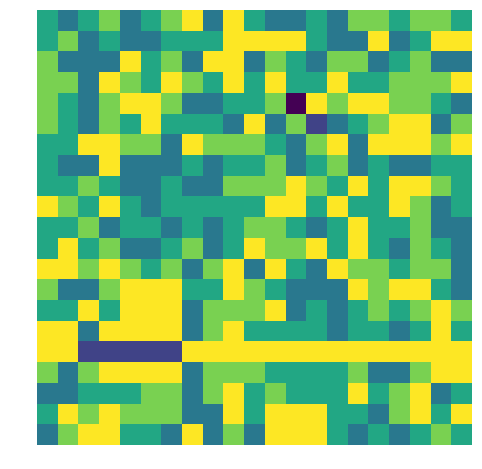
\includegraphics[width=3cm]{./Images/Chapter08/catch_v3} }}%
     \qquad
    \subfloat[\centering label 4]{{
\includegraphics[width=3cm]{./Images/Chapter08/catch_v1} }}% 
    \caption{2 Figures side by side}%
    \label{fig:example}%
\end{figure}


\subsection{From one Catcher to Another}

\subsection{Self-Transfer}
 % ICML (under review) paper?
%Chapter 7

\chapter{Concluding Remarks} % Chapter title
\label{ch:upside_down_rl} % For referencing the chapter elsewhere, use \autoref{ch:introduction} 

\begin{remark}{Outline}
This is the final chapter of this dissertation which is divided in two parts: we start by answering the research questions that were presented at the beginning of this work in Chapter \ref{ch:introduction} in Sec. \ref{sec:answers}. Each question is answered with respect to the research that has been presented throughout the earlier chapters of this work and is followed by a brief critical conclusion. We then move to the second part of this chapter presented in Sec. \ref{sec:critical_discussion}, where we will critically analyze how over the last decade, the fields of supervised learning and reinforcement learning have been affected by the rise of deep neural networks and describe what the future of both research fields could look like in the coming years. 
\end{remark}


\section{Answers to the Original Research Questions}
\label{sec:answers}

We now answer the research questions that we have originally introduced in Chapter \ref{ch:introduction} and that have served as inspiration for all the work presented throughout this thesis.

\begin{enumerate}
	\item \textit{"Can convolutional neural networks be transferred and trained across different source and target domains? \\ if so, which target domains could be of interest for investigating their transfer learning properties?"}
	
	The research presented in Chapters \ref{ch:tl_natural_to_non_natural}, \ref{ch:minerva} and \ref{ch:tl_lth} shows that when it comes to supervised learning problems, convolutional neural networks exhibit strong transfer learning properties. In Chapter \ref{ch:tl_natural_to_non_natural} we have in fact seen that five popular neural architectures, originally designed for tackling computer vision problems on datasets containing natural images, can be transferred for targetting classification problems that come from the field of digital heritage. Furthermore, we have also empirically shown that all such pre-trained architectures, are able to learn features on datasets of natural images that generalize to the non natural image domain. Similar conclusions can also be drawn from the results presented in Chapter \ref{ch:minerva}, where we have shown that the good transfer learning properties of convolutional neural networks go beyond the computer vision task of classification, and also hold for object detection problems. Similarly to the research presented in Chapter \ref{ch:tl_natural_to_non_natural} we have again considered the field of digital heritage as target domain, as it offers numerous potentially interesting practical applications such as e.g., the one described by the MINERVA dataset. In Chapter \ref{ch:tl_lth} we have then seen that an equally important target domain for exploiting the transfer learning properties of pre-trained image classifiers is that of digital pathoology, as it is a field that is potentially characterized by a lack of appropriate training data, a hurdle that can strongly limit the training process of a convolutional neural network.

	While all the research presented in the second part of this thesis provides strong evidence in favour of transferring, and potentially fine-tuning, pre-trained convolutional neural networks, the same can however not be said for the results obtained in Chapter \ref{ch:dqn_transfer}, where we have instead seen that the transfer learning potential of such models can be much more limiting when it comes to the reinforcement learning domain. 

	
	\item \textit{"What Transfer Learning training strategy should be adopted to maximize the performance of pre-trained networks?"}

	As presented in Chapter \ref{ch:transfer_learning}, there are two main approaches for performing transfer learning in the context of convolutional neural networks: an off-the-shelf feature extraction approach, and a fully fine-tuning approach. The research presented in Chapter \ref{ch:tl_natural_to_non_natural} clearly shows that when it comes to image classification problems, the latter training strategy results in significantly better final performance, as it allows networks to better adapt to the target domain, and therefore learn new feature representations that are relevant for the target task. The results of this study served as inspiration for the research presented in Chapter \ref{ch:minerva} where a fine-tuning training strategy was preferred over an off-the-shelf approach when tackling object detection problems and, in the end, resulted in models that were able to successfully detect musical instruments in paintings. Surprisingly, however, in Chapter \ref{ch:dqn_transfer} we have then seen that a fine-tuning transfer learning approach can be detrimental in the context of model-free deep reinforcement learning, as deep reinforcement learning agents transfer very poorly across tasks and even to themselfes. In the case of the latter, however, this only happens if a fine-tuning training strategy is adopted and not if the networks are used as simple feature extractors.   

Despite the negative performance presented in Chapter \ref{ch:dqn_transfer} we overall still believe that if enough computational resources are available, pre-trained convolutional neural networks should always be fine-tuned, especially when it comes to supervised learning problems.

	\item \textit{"Can Transfer Learning be a valuable tool for better understanding convolutional neural networks?"}
	
	Throughout this thesis we have argued that convolutional neural networks should be studied from a transfer learning perspective, not only because this would allow practictioners to know whether such algorithms could be deployed to real world applications, but also because their transfer learning properties could deliver novel insights into their inner properties. The research presented in Chapters \ref{ch:tl_lth} and \ref{ch:dqn_transfer} is a clear example that shows that a better understanding of convolutional neural networks can be obtained thanks to transfer learning. In Chapter \ref{ch:tl_lth} we have used transfer learning as a tool for better understanding the phenomenon of the Lottery Ticket Hypothesis (LTH). This allowed us to show that pruned convolutional neural networks winners of the LTH contain inductive biases that are generic at least to some extent, and therefore gain a deeper understanding of this deep learning phenomenon. In Chapter \ref{ch:dqn_transfer} we have instead discovered that convolutional neural networks transfer very poorly when they get trained for solving reinforcement learning tasks in a model-free deep reinforcement learning setting. With the intent of understanding why their transfer learning potential was not on par with the one that was extensively observed in Chapters \ref{ch:tl_natural_to_non_natural} and \ref{ch:minerva}, we have gained novel insights that allowed us to show that models commonly denoted as Deep-Q Networks go through two very distinct training phases. 

We therefore believe that transfer learning is an extremely valuable tool for better understanding neural networks, as it allows to study their training process from a perspective which is unique and that goes beyond that of models that get trained from scratch.  

	
	\item \textit{"Do different machine learning paradigms result in convolutional neural networks with different transfer learning properties?"}

	Based on the significant gap in terms of performance between the results obtained in the second part of this dissertation, and the results obtained in the third part of this thesis, we strongly believe that the answer to this research question is \textit{yes}. Specifically, we have seen that as long as convolutional neural networks are trained for solving supervised learning tasks, then they will very likely exhibit strong transfer learning properties (see Chapters \ref{ch:tl_natural_to_non_natural} and \ref{ch:minerva}). However, if such models will be used for tackling deep reinforcement learning problems in a model-free reinforcemnt learning context, then their transfer learning potential will be much more limited. The reason of this is that when it comes to supervised learnig, convolutional neural networks will only have to serve as feature extractors, whereas the same cannot be said for model-free deep reinforcement learning, where such models have also to serve as optimal value function approximators. 

The transfer learning potential of convolutional networks is therefore highly dependant from the machine learning problem at hand, although we also believe that the poor transfer learning properties observed in Chapter \ref{ch:dqn_transfer} are inherent to model-free deep reinforcement learning algorithms only.


\end{enumerate}


\section{Critical Discussion \& Future Perspectives}
\label{sec:critical_discussion}

We now present a critical discussion which addresses some of the limitations that currently characterize the fields of deep supervised and deep reinforcement learning and see how they relate to possible future work.

\subsection{Deep Supervised Learning}
\label{sec:supervised_learning}

\paragraph{Data and Computing Power:}
Neural networks only require two simple ingredients for tackling most of supervised learning problems: 1) large amounts of training data and 2) enough computational resources. If both of such ingredients are available, we believe that any supervised learning problem can be addressed successfully, and that the field of supervised machine learning can be considered as solved. While it is true that both ingredients can not always be available to machine learning practitioners, it is also true that as extensively demonstrated throughout the second part of this thesis, one could overcome their scarcity thanks to deep transfer learning. We therefore disagree with \citet{marcus2018deep} who at the present moment considers the deep learning field as too data hungry, and believe that this is an issue that thanks to the availability of large pre-trained models has been successfully addressed.  

\paragraph{Interpretability:}
High accuracies and reduced computation times are, however, not the only properties which are desirable in a machine learning model. Deep neural networks are often considered as black box models, and as mentioned by \citet{marcus2018deep} one of their limitations is that they are not transparent enough, a property which is desirable in fields such as medicine and finance. We agree that this is a limitation that at the present moment is part of neural networks, and can easily imagine the field of Explainable Artificial Intelligence (XAI) providing some solutions in this regard in the next years. However, differently from \cite{adadi2021survey} we do not believe that this will be achieved by integrating symbolic AI techniques within neural networks, but rather through the development of novel visualization techniques such as the ones adopted in Sec. \ref{sec:qualitative_analysis} of Chapter \ref{ch:minerva}. 

\paragraph{On the Future of Convolutional Neural Networks:}
As extensively documented throughout this dissertation, when it comes to classification and regression problems that are characterized by high-dimensional inputs, convolutional neural networks have become the de facto neural architecture. Yet, over the last years newer models such as Vision Transformers (ViTs) \cite{dosovitskiy2020image} and Graph Neural Networks (GNNs) \cite{scarselli2008graph,kipf2016semi,garcia2017few,scarselli2005graph} have started to obtain excellent performance. The first one appear to be requiring substantially fewer computational resources for training, while the latter are particularly well suited for problems where it is important to exploit structural relationships within data. We believe that in the coming years both type of models will gain popularity, but also that these kind of architectures will always be combined with convolutional neural networks. In fact, we hardly imagine that there will ever be a neural architecture which exploits inductive biases as much as convolutional networks and that is able to perform equally well in a deep transfer learning setting.   

\subsection{Deep Reinforcement Learning}
\paragraph{Tedious Hyperparameters}

In Chapter \ref{ch:reinforcement_learning} we have seen that Deep Reinforcement Learning (DRL) has gained a lot of attention from the machine learning community over the last decade, as the number of successful applications showcasing its potential have in fact become countless, ranging from agents achieving super-human performance on popular boardgames such as chess and go, to neural networks able to autonomously navigate stratospheric balloons. To an untrained eye, or more simply to a RL practitioner with few years of experience, successfully training a DRL agent might look like a straightforward task. However, behind the largely acclaimed accomplishments praised by the DRL literature, there is an equivalently large, and mostly hidden, process of hyperparameter tuning which is essential for successfully training a neural network. Throughout this thesis, convolutional neural networks have been trained both in a supervised learning context as well as in a reinforcement learning one, and we have in first person experienced how unrobust and oversensitive such algorithms can be when targeting the latter type of problems. This susceptability, on the contrary, was never encountered when tackling supervised learning tasks. We believe that at the present moment, despite all of its remarkable achievements, DRL cannot yet be considered as a successful application of convolutional neural networks. As long as a state of the art Rainbow agent \cite{hessel2018rainbow} can only get successfully trained if its learning rate is set to the unintuitive value of $0.0000625$, and a DRL practitioner has to wait for weeks before being able to see a DQN agent play certain games of the Atari Arcade Learning Environment \cite{kaiser2019model}, we believe that DRL is far from being solved.


\paragraph{The Deadly Triad}
In Chapters \ref{ch:reinforcement_learning} and \ref{ch:dqv_family_of_algorithms} we have mentioned the Deadly Triad of Deep Reinforcement Learning, a combination of three elements, which if present within the same learning agent can result into algorithms that diverge and are unable to learn an approximation of an optimal value function. As one of the elements of the Deadly Triad is that of a function approximator, it naturally follows that the stability of deep reinforcement learning algorithms will constantly be questioned by the deep learning community which will regularly introduce novel neural architectures in the coming years. This raises the natural question \textit{`which element of the triad should eventually be given up when developing DRL algorithms?"}. So far, the community seems to agree that giving up on function approximators is clearly not possible as neural networks will always play a crucial role in the development of future DRL algorithms \cite{van2018deep_triad,hernandez2019understanding,fedus2020revisiting} thanks to their properties that we discussed in Sec. \ref{sec:function_approximators} of Chapter \ref{ch:reinforcement_learning}. We agree with this point of view and therefore believe that either off-policy learning or bootstrapping should be given up: if the end goal is that of developing algorithms that do not diverge whilst training we believe that it is the off-policy learning element of the triad which should be withdrawn during the development of novel DRL techniques. While this could come at the price of restricting the number of possible policies that could be learned by an agent, we believe that this is a problem which could be controlled as long as agents will be combined with proper exploration policies. The DQV-Learning algorithm presented in Chapter \ref{ch:dqv_family_of_algorithms} is an example of a DRL algorithm that can avoid divergence through on-policy learning, while at the same time making use of a neural network trained through temporal-difference learning. 


\paragraph{Reinforcement Learning Upside Down}

It is clear that the combination of reinforcement learning algorithms and deep neural networks can present some significant limitations. Throughout this dissertation we have mainly focused on the aforementioned Deadly Triad phenomenon and on the poor transfer learning properties of Deep-Q Networks which both can limit the development of robust and general agents. Next to these issues, DRL algorithms are characterized by numerous other problems as well (the discussion of which is out of the scope of this thesis) and that all mainly arise because tabular RL algorithms are combined with function approximators \cite{tsitsiklis1997analysis,van2016deep,anschel2017averaged,fujimoto2018addressing,fujimoto2019benchmarking, kumar2019stabilizing, marklundexact}. Although the DRL community has been able to address most of such issues successfully, we believe that the way optimal control problems are currently being solved by the DRL community might need revision. In fact, we argue that most of the current DRL research focuses on introducing solutions that, albeit valuable, are only able to solve very specific and limited problems to a (sometimes very) small extent. As a result, very few DRL practitioners have been critically questioning the long term value of modern DRL algorithms, and the way RL problems are currently being addressed. An exception to this common trend, however, has recently been introduced by \citet{schmidhuber2019reinforcement} who proposed the idea of `Upside-Down Reinforcement Learning" (UDRL). In UDRL the main goal is to solve typical Markovian control problems via classic supervised learning techniques, and to replace common RL concepts such as value function approximation and policy search, through maximum likelihood estimation techniques. In principle this should be done by learning a mapping from states to actions (see \cite{srivastava2019training} for all the mathematical details), which could overcome the need of learning an optimal value function or stochastic policy. We agree with Schmidhuber's ideas, and support the goal of potentially solving optimal control problems via supervised learning techniques. In fact we strongly believe that DRL in its current form is already reducing reinforcement learning problems to supervised learning problems. As an example let us consider the role of the experience replay memory buffer reviewed in Chapter \ref{ch:reinforcement_learning} and adopted by the DQV and DQV-Max Learning algorithms presented in Chapter \ref{ch:dqv_family_of_algorithms}. We have seen that the role of experience replay is that of storing RL trajectories which can in a later moment be sampled and used for minimizing the objective function of a Deep-Q Network. By taking a critical look at this buffer, we can see that it is in large part equivalent to the datasets that are typically used in supervised learning: it needs to store a large amount of RL trajectories which can then be used for modeling the task of learning a value function as a regression problem where $\mathcal{Y}$ is modeled by the space of all TD-errors stored within the buffer. The idea of constructing a dataset of previous trajectories is very far from the ideal RL setting reviewed at the beginning of Chapter \ref{ch:reinforcement_learning}, where we have indeed seen that a RL agent should be able to learn in an online fashion based on the last trajectory only. We therefore believe that the successess obtained by DRL stem from the fact that RL problems have been modeled as supervised learning ones, which as discussed in Sec. \ref{sec:supervised_learning} are well suited for deep neural networks.

We have experimented with some of the UDRL ideas presented in \cite{schmidhuber2019reinforcement,srivastava2019training} and compared the performance of a preliminary version of an UDRL agent to that of a DQN, DDQN and DQV agent on two different benchmarks: the popular control problem \texttt{Cartpole} and the Atari game \texttt{Pong}. We report the results of these very preliminary experiments in Fig. \ref{fig:upside_down_results}. We can see that on the \texttt{Cartpole} benchmark the UDRL learns significantly better than all three model-free DRL algorithms, but is unable to improve its policy over time at all when it comes to the more complicated \texttt{Pong} game. These results show that UDRL has definitely some potential, although furhter research will be required to investigate whether this type of algorithm can scale to more complicated problems. We believe that if such scaling issues will be solved, then UDRL could become a valid alternative to popular DRL algorithms. More specifically we foresee that in the future UDRL will find a successful application in the following three RL areas: \footnote{Please note that these claims are at the present moment not empirically supported in any way, and are made on top of some intuition that has been built after performing the preliminary experiments presented in Fig. \ref{fig:upside_down_results}.}.

\begin{figure}[ht!]
  \begin{tikzpicture}[scale = 0.65]
      \begin{axis}[
	name=ax1,
	grid style={dashed,gray},
      	grid = both, 
      	tick style=black,
	title=Cartpole,
        xlabel=Episodes,
        ylabel= Reward,
      ]

      \addplot [ultra thick, red, mark=.] table [y=DQV, x=episodes]
      {./Results/Chapter09/logs/cartpole_results.txt};
      \addplot [ultra thick, blue, mark=.] table [y=DQN, x=episodes]{./Results/Chapter09/logs/cartpole_results.txt};
      \addplot [ultra thick, green, mark=.] table [y=DDQN, x=episodes]{./Results/Chapter09/logs/cartpole_results.txt};
      \addplot [ultra thick, cyan, mark=.] table [y=Upside-Down, x=episodes]{./Results/Chapter09/logs/cartpole_results.txt};
      \end{axis}

      \begin{axis}[
	at={(ax1.south east)},
	xshift=2cm,
	grid style={dashed,gray},
      	grid = both, 
      	tick style=black,
	title=Pong,
        xlabel=Episodes,
        ylabel= Reward,
        legend columns=4, 
        legend style={font=\Large, at={(-0.9,-0.3,-0.4)},anchor=north west,legend columns=4},
      ]

      \addlegendentry{DQV}
      \addlegendentry{DQN}
      \addlegendentry{DDQN}
	\addlegendentry{Upside-Down RL} 

      \addplot [ultra thick, red, mark=.] table [y=DQV, x=episodes]
      {./Results/Chapter09/logs/pong_results.txt};
      \addplot [ultra thick, blue, mark=.] table [y=DQN, x=episodes]{./Results/Chapter09/logs/pong_results.txt};
      \addplot [ultra thick, green, mark=.] table [y=DDQN, x=episodes]{./Results/Chapter09/logs/pong_results.txt};
      \addplot [ultra thick, cyan, mark=.] table [y=Upside-Down, x=episodes]{./Results/Chapter09/logs/pong_results.txt};
 
      \end{axis}
	\end{tikzpicture}
	\caption{Two examples of an UDRL agent described by \citet{schmidhuber2019reinforcement}. When combined with a multi-layer perceptron the agent significantly outperforms the DQV, DQN and DDQN agents on the Cartpole environment (left figure). However, it is unable to improve its policy over time at all when trained on the Pong game and combined with a convolutional neural network (right figure).}
	\label{fig:upside_down_results} 
\end{figure}



\begin{itemize}
	\item \textcolor{RoyalBlue}{Transfer Learning}: as neural networks will not have to jointly serve as optimal value function approximators and feature extractors, we believe that UDRL agents should in principle be more suitable for transfer learning. In fact such models will not have to go through the training dynamics that we have identified in Chapter \ref{ch:dqn_transfer}, and will in essence be more similar to the type of models that we have successfully transferred throughout the second part of this dissertation (as they will be trained according to supervised learning principles).  
	\item \textcolor{RoyalBlue}{Batch Reinforcement Learning}: a common problem of current DRL algorithms is that they suffer from a phenomenon known as `extrapolation error" \cite{fujimoto2019benchmarking}. When such agents are trained in a batch setting, they fail in improving their policy because the trajectories contained within the experience replay memory buffer have been collected by a different agent. This can pose numerous practical issues as the process of collecting RL trajectories can sometimes be particular expensive, therefore limiting the potential interaction between the agent and its environment. As UDRL technically overcomes the need of learning an optimal value function, it follows that such agents should not suffer from the extrapolation bias and could therefore generalize well in a batch RL set-up.   
	\item \textcolor{RoyalBlue}{Interpretable Reinforcement Learning}: the main training principle of UDRL agents of maximum likelihood estimation opens the door to the use of supervised learning algorithms other than deep neural networks. Deep neural networks are often considered to be black boxes and highly uninterpretable models, which is a quality that when it comes to optimal decision making problems could be desirable \cite{mott2019towards}. However, supervised learning algorithms that are largely more interpretable than neural networks do already exist \cite{}, and we therefore foresee that these could be used in combination with UDRL in situations where it is desirable to interpret the decision taken by an agent.
\end{itemize}
  

\begin{takeaway}{Takeaway of Part III}

\end{takeaway}







 % Upside-Down RL + critical discussion



\cleardoublepage % Empty page before the start of the next part

%----------------------------------------------------------------------------------------
%	THESIS CONTENT - APPENDICES
%----------------------------------------------------------------------------------------

\appendix

\part{Appendix} % New part of the thesis for the appendix

%% Appendix A

\chapter{Appendix Test}

%----------------------------------------------------------------------------------------

\lipsum[13-14]

%----------------------------------------------------------------------------------------

\section{Appendix Section Test}
\lipsum[15]

\graffito{More dummy text}
\lipsum[16]

%----------------------------------------------------------------------------------------

\section{Another Appendix Section Test}
\lipsum[17]

\begin{table}
\myfloatalign
\begin{tabularx}{\textwidth}{Xll} \toprule
\tableheadline{labitur bonorum pri no} & \tableheadline{que vista}
& \tableheadline{human} \\ \midrule
fastidii ea ius & germano &  demonstratea \\
suscipit instructior & titulo & personas \\
\midrule
quaestio philosophia & facto & demonstrated \\
\bottomrule
\end{tabularx}
\caption[Autem usu id]{Autem usu id.}
\label{tab:moreexample}
\end{table}

\lipsum[18]

There is also a useless Pascal listing below: \autoref{lst:useless}.

\begin{lstlisting}[float=b,language=Pascal,frame=tb,caption={A floating example (\texttt{listings} manual)},label=lst:useless]
for i:=maxint downto 0 do
begin
{ do nothing }
end;
\end{lstlisting} % Appendix A
% Appendix X

\chapter*{Appendix}
\label{ch:appendix}


\section{The Deep Quality-Value Learning Algorithms}
\begin{algorithm*}
\footnotesize
\caption{DQV and DQV-Max Learning}\label{alg: dqv_algorithms}
\begin{algorithmic}[1]
\Require{Experience Replay Queue $D$ of maximum size $N$}{}
\Require{$Q$ network with parameters $\theta${}} \Comment{Network required by DQV}
\Require{$V$ networks with parameters $\Phi$ and $\Phi^{-}$ {}} \Comment{Networks required by DQV}
\Require{$Q$ networks with parameters $\theta$ and $\theta^{-}${}} \Comment{Networks required by DQV-Max}
\Require{$V$ network with parameters $\Phi${}} \Comment{Network required by DQV-Max}
\Require{total\_a = 0}
\Require{total\_e = 0}
\Require{c = $10000$}
\Require{$\mathcal{N} = 50000$}

\While{True}
\State{set $s_t$ as the initial state}
\While{$s_t$ is not terminal}
    \State{select $a_t\in\mathcal{A}$ for $s_{t}$ with policy $\pi$ (using the epsilon-greedy strategy)}
    \State{get $r_{t}$ and $s_{t+1}$}
    \State{store $\langle s_{t}, a_{t}, r_{t}, s_{t+1}\rangle$ in $D$}
    \State{$s_t := s_{t+1}$}
    \State{total\_e += 1}
    \If{total\_e $\geqq \mathcal{N}$}
            \State{sample a minibatch $B=\{\langle s^i_t, a_t^i, r^i_t, s^i_{t+1}\rangle|i=1,\ldots,32\}$ of size 32 from $D$}
        \For{i = 1 to 32}
        \If{$s^i_{t+1}$ is terminal}
            \State{$y^i_{t} := r^i_{t}$}    \Comment{TD-Error for DQV}
            \State{$v^i_{t} := r^i_{t}$}    \Comment{1st TD-Error for DQV-Max}
            \State{$q^i_{t} := r^i_{t}$} \Comment{2nd TD-Error for DQV-Max}
        \Else
            \State{$y^i_{t} := r^i_{t} + \gamma V(s^i_{t+1}, \Phi^{-})$} \Comment{TD-Error for DQV} 
            
            \State{$v^i_{t} := r^i_{t} + \gamma \: \underset{a\in \mathcal{A}}{\max}\: Q(s^i_{t+1}, a, \theta^{-})$} \Comment{1st TD-Error for DQV-Max}
            \State{$q^i_{t} := r^i_{t} + \gamma \: V(s^i_{t+1}, \Phi)$} \Comment{2nd TD-Error for DQV-Max}
         \EndIf
         \EndFor
        \State{$\theta := \underset{\theta}{\argmin} \sum_{i=1}^{32} (y^i_{t} - Q(s^i_{t}, a^i_{t}, \theta))^{2}$}
        \Comment{Train the $Q$ network for DQV}
        \State{$\Phi := \underset{\Phi}{\argmin} \sum_{i=1}^{32}(y^i_{t} - V(s^i_{t}, \Phi))^{2}$}
        \Comment{Train the $V$ network for DQV}
         \State{$\theta := \underset{\theta}{\argmin}\: \sum_{i=1}^{32} (q^i_{t} - Q(s^i_{t}, a^i_{t}, \theta))^{2}$}
         \Comment{Train the $Q$ network for DQV-Max}
        \State{$\Phi := \underset{\Phi}{\argmin}\: \sum_{i=1}^{32} (v^i_{t} - V(s^i_{t}, \Phi))^{2}$}
        \Comment{Train the $V$ network for DQV-Max}
        \State{total\_a += 1}
        \If{total\_a = $c$}
            \State{$\Phi^{-}$ := $\Phi$} \Comment{Update the target $V$ network in DQV}
            \State{$\theta^{-}$ := $\theta$} \Comment{Update the target $Q$ network in DQV-Max}
            \State{total\_a := 0}
         \EndIf
    \EndIf
\EndWhile
\EndWhile

\end{algorithmic}
\end{algorithm*}




%----------------------------------------------------------------------------------------

% Content begins here
 % Appendix B - empty template

%----------------------------------------------------------------------------------------
%	POST-CONTENT THESIS PAGES
%----------------------------------------------------------------------------------------

\cleardoublepage% Bibliography

\label{app:bibliography} % Reference the bibliography elsewhere with \autoref{app:bibliography}

\manualmark % Work-around to have small caps also here in the headline
\markboth{\spacedlowsmallcaps{\bibname}}{\spacedlowsmallcaps{\bibname}} % Work-around to have small caps also
%\phantomsection
\refstepcounter{dummy}

\addtocontents{toc}{\protect\vspace{\beforebibskip}} % Place the bibliography slightly below the rest of the document content in the table of contents
\addcontentsline{toc}{chapter}{\tocEntry{\bibname}}

\printbibliography % Bibliography


%\cleardoublepage% Colophon (a brief description of publication or production notes relevant to the edition)

\pagestyle{empty}

\hfill

\vfill

\pdfbookmark[0]{Colophon}{colophon}

\section*{Colophon}

This document was typeset using the typographical look-and-feel \texttt{classicthesis} developed by Andr\'e Miede. The style was inspired by Robert Bringhurst's seminal book on typography ``\emph{The Elements of Typographic Style}''. \texttt{classicthesis} is available for both \LaTeX\ and \mLyX: 

\begin{center}
\url{https://bitbucket.org/amiede/classicthesis/}
\end{center}

\noindent Happy users of \texttt{classicthesis} usually send a real postcard to the author, a collection of postcards received so far is featured here: 

\begin{center}
\url{http://postcards.miede.de/}
\end{center}
 
\bigskip

\noindent\finalVersionString % Colophon

%----------------------------------------------------------------------------------------

\end{document}
